\chapter{Activity Allocation (AA) Module}\label{sec:aa-module-chapter}
The Activity Allocation (AA) module represents the regional economic relationships among industry, households and institutions within the model. It includes the economic allocation portion of the Production, Exchange, and Consumption Allocation System (PECAS) developed by \cite{hunt05}. In each period, AA takes the aggregate modelwide activity totals (2009 dollars of production and imports/exports) from the NED module, counts of modelwide households from the SPG1 module, the available floorspace by alpha zone from the ALD module and travel accessibilities from the PT module and VISUM locates the various actors (industry and households), generates a set of economic flow matrices for each commodity and determines the technology (the commodities made and used including labor and floorspace) for each activity for each beta zone (called land use zone \textit{LUZ} in AA). AA also determines the quantity of floorspace occupied by industry and households, given a fixed floorspace supply inventory from the ALD module. 

AA labor flows are used in the SPG module to locate households (home end) and in the PT module to locate workplaces (work end). The flow of goods (including imports and exports) is used by the CT module. These uses are employed in the current year, while ALD uses AA allocation of demand in the prior two years to allocate regional construction dollars among 15 regions and prior year vacancy rates and prices to identify the floorspace types and zonal location for such development. A future Economic Feedback (EF) module will makes use of the overall quality of industry operations (AA logsums) to influence the NED regional forecast totals in the next year. Finally, the previous year AA-generated location of activities influences current-year AA activity location decisions.

AA also runs once before the base year as part of the bootstrap process. This run is constrained to reproduce observed activity distributions by beta zone. It writes constants to the ActivityLocations file that modify the behavior of AA in later years. The constrained run helps incorporate influences on activity location that are hard to measure directly, so that activities are more likely to be allocated to places where they exist in real life even if the location seems unjustified economically.

The overall approach to the allocations done in the AA module was represented diagrammatically in Figure \ref{fig:make-use-summary} (page \pageref{fig:make-use-summary}). Commodities (columns) are produced and consumed (goods, services, labor, floorspace) both for the study area and for import and export. Economic actors (rows) (industries, government, households) separately account for import make and export use activities in addition to modelwide make and use.

\section{Theoretical Basis}\label{sec:aa-theoreticals}
The Activity Allocation Module (AA Module) is an aggregate representation based on spatially-disaggregated forms of extended input-output make and use tables, with variable technical coefficients.  This approach represents a specialized adaptation of a social accounting matrix. AA concerns quantities of activities, flows of commodities and markets with aggregate demands and supplies and exchange prices.

Activities are located in land use zones (LUZ or beta zone). Activities produce commodities and then transport and sell these commodities; and they also consume commodities after buying them and transporting them.  There are different types of activities, including industrial sectors, government and households. Activity quantities can be measured in values (for example, dollars of business repair industrial activity) or numbers (for example, number of households with high income and 2 or less persons). The AA Module allocates the study-area wide quantity of each activity among the beta zone as part of its allocation process.

Commodities flow at specific rates from where they are produced to where they are exchanged (from seller to buyer), and then from where they are exchanged to where they are consumed. Commodities are grouped into categories, including different types of goods and services, labor and space. Commodities other than floorspace in general flow across zone boundaries. Floorspace is restricted in that it is ``non-transportable'' and must be exchanged and consumed in the beta zone where it is produced, which means that the space commodity categories receive some special additional treatments in PECAS.  Commodity flows are measured in values per unit time (for example, dollars of management services per year) or numbers per unit time (for example, tons of coal per month). The movement of these flows of commodities from where they are produced to where they are consumed is the economic basis for travel and transport in the modeling system.  It is the travel conditions --- the distances, costs, times and associated (dis)utilities by mode --- for the movement of these commodities that results in the influence of the transportation system on the interactions among activities and the attractiveness of locations for activities.  The AA Module allocates the flows of commodities from production location beta zone to exchange location beta zone and from exchange location beta zone to consumption location beta zone, and finds the corresponding set of prices at the exchange location beta zone that clears all markets, as part of its allocation process.

Activities produce commodities and consume commodities in the production process according to the technology they use.  More specifically, an activity quantity in a given beta zone produces commodities at specific rates per unit of activity and consumes commodities at specific rates per unit of activity according to the technology being used by the activity. One or more ``technology option'' alternatives are defined for a given activity (industry or household). Each of these technology options is a specific vector of production and consumption rates for different commodities per unit of the activity, representing a particular technology option for the production process available to the activity. The AA Module allocates the quantity of the activity in each beta zone among these ``technology options'' as part of its allocation process.

The allocation process in the AA Module uses a three-level nested logit model with a nesting structure as shown in Figure \ref{fig:aa-nesting-structure}.

\begin{figure}[!t]
\centering
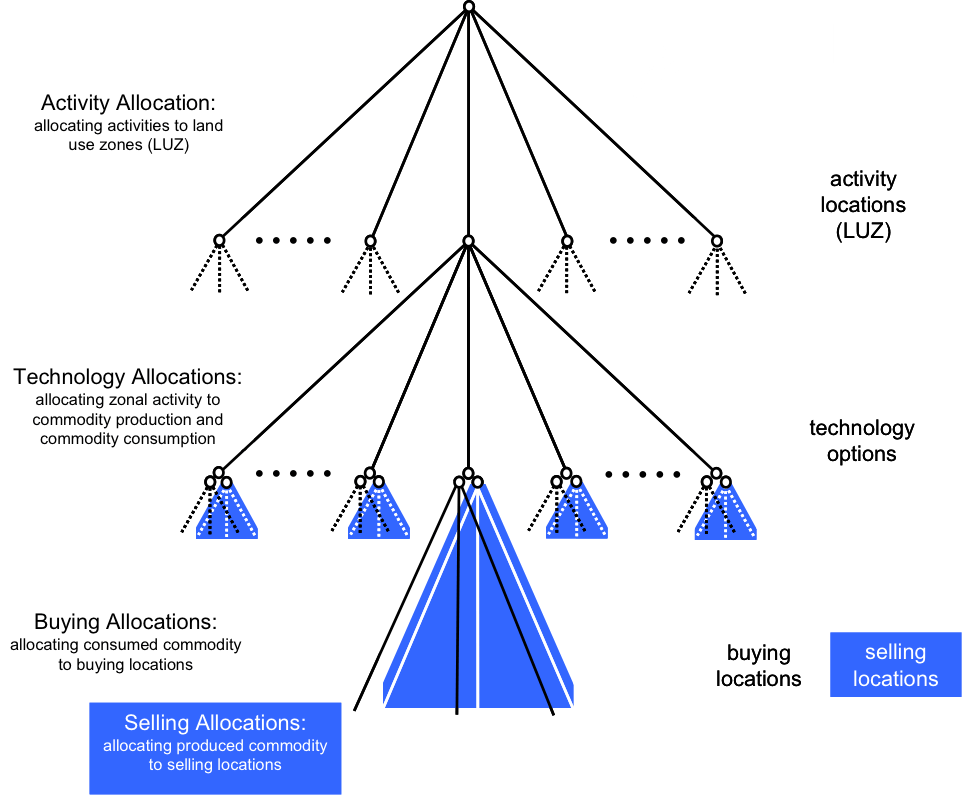
\includegraphics[scale=0.45]{aa/nesting-structure}
\caption{Three-level nesting structure used in allocations }\label{fig:aa-nesting-structure}
\end{figure}

At the highest level of the nesting structure, the study-area total quantity of each activity is allocated among the beta zone. At the middle level, the quantity of each activity in each beta zone is allocated among the available technology options. At the lowest level, there are two logit allocations for each commodity in each beta zone: The first is an allocation of the produced quantities among the various exchange locations where they are sold to other activities; the second is an allocation of the consumed quantities among the various exchange locations where they are bought by other activities.

At the lowest level, the utility of each exchange location alternative is influenced by the price at the exchange location and the characteristics for transporting the commodity to or from the exchange location.  The composite utility values from these two lowest-level logit models are called the ``buying utility'' and the ``selling utility'' for the commodity in the beta zone. They are used as the transportation-related inputs in the middle-level for allocating the activities in the beta zone among the relevant technology options. The composite utility value for the range of technology options considered at the middle-level for an activity in a beta zone is part of the location utilities used at the highest-level.

The spatial aspects of the AA Module allocation process are illustrated in Figure \ref{fig:aa-spatial-aspects}. Buying and selling allocations link through the exchange locations to establish commodity flows from production to consumption locations in the beta zone.

\begin{figure}   % Originally Figure 6.2
\centering
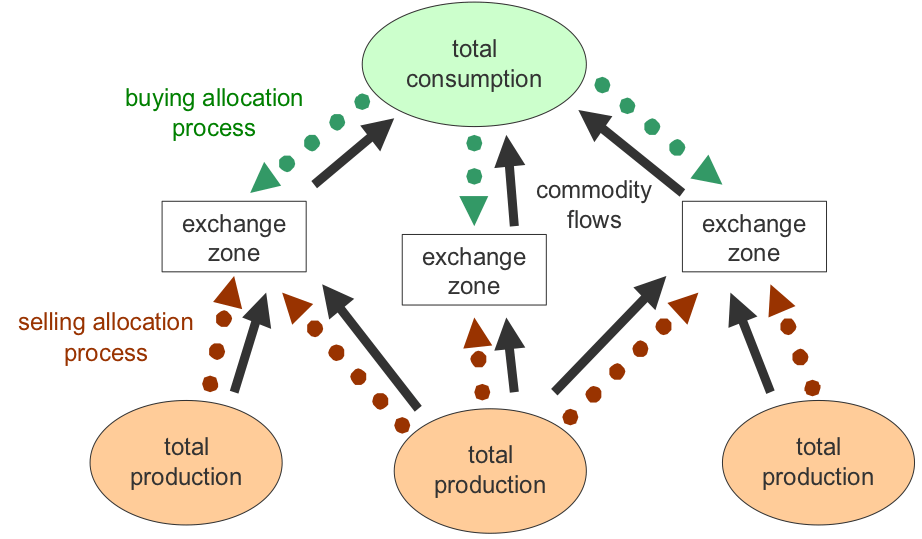
\includegraphics[scale=0.35]{aa/spatial-aspects}
\caption{Buying and selling allocations resulting in commodity flows}\label{fig:aa-spatial-aspects}
\end{figure}

The exchange locations are location-specific markets for commodities, where sellers sell commodities to buyers. Prices are established at exchange locations so that the quantity bought equals the quantity sold. Thus, the spatial allocation procedure in the AA Module assumes a short-run market equilibrium in commodities.

In the general case, commodities can be assigned in any of the available exchange zones (either all the zones in the model or a specified set of 1 or more exchange zones). For simplicity and realism, commodities can be assigned to be either (a) purchased from the exchange location in the beta zone where they are consumed (e.g. for labor, this occurs in the employment zone, where the labor is exchanged and the price set), or (b) purchased in the exchange location in the beta zone where they are produced (e.g. for retail goods this is at the retail establishment, where the goods are exchanged and the price is set), or (c) produced, exchanged and consumed in the same zone (e.g. for floorspace which is attached to the ground and cannot be moved). In these cases for each commodity in each zone, one (or both) of the logit allocation models (either the buying or the selling) consists of only one alternative.

The import and export of goods commodities that are physically transported by vehicles enter the system at six specific external exchange locations termed World Markets. The import and export quantity at each external World Market and internal exchange location are determined as functions of the exchange price in both locations, so that as prices rise more imports are attracted and as prices fall more exports are produced. The import and export functions tie the economy in the model to the rest of the world.

\section{Quantity Definitions and Categories}

AA operates at the beta zone level, although some outputs are expanded to the alpha zone level (see Figure \ref{fig:swim2-model-area} on page \pageref{fig:swim2-model-area}) for use in the SPG2 and PT modules. For import and export of goods commodities, AA uses a set of six world market zones, which are allocated to 12 external stations in the CT modules for network assignment. World markets were defined in Table \ref{tab:world-markets} and mapped in Figure \ref{fig:world-markets}. % and \ref{figure_2.4}.

AA uses the industry and household activity categories of Table \ref{tab:activity-industry} and \ref{tab:size-income} and goods, services, labor and floorspace commodity categories defined in Tables \ref{tab:service-categories} through \ref{tab:goods-categories} (pages \pageref{tab:activity-industry}--\pageref{tab:goods-categories}). Additional actors are used only in the AA and NED modules to complete the accounting of money flows. These include aspatial money flow government activities: FGOV\_acct\_gov, SLGOV\_acct\_gov, CAP\_acct\_gov, and associated aspatial activities in the eduction, investment and energy permitting sectors.

The commodity flows associated with these activities do not interact with the transportation system and have zero transport costs (money moves for free), so they are exchanged in only one zone (assumed at the alpha zone location of the state capital in Salem, OR) and do not add to the runtime of the software. For instance, ``Education reports to sponsors'' was added to track the funding of schools by governments and the responsibilities of schools to serve not only the students but also their funders. (The education flow of students going to school to be taught was renamed to ``Teaching K12'' to make it distinct from the flow of funding.)  Some inputs exist to allow GHG Permits (Greenhouse Gas Permits) to be added to the model in a future version, to support scenarios designed to understand the effect of an imposed price or cap on greenhouse gas emissions. The full set of aspatial financial flows includes:
\begin{itemize}
\item Education Reports to Sponsors,
\item Government Support Receipts
\item Tax Receipts,
\item Investing Receipts, 
\item Return Investment Receipts,
\item Capital Transfer Receipts,
\item Proprietor Income Receipts,
\item GHG Permits (Greenhouse Gas Permits) (not included in the current version)
\end{itemize}

\section{Component Models}

The objective of the AA module is to find a market clearing price equilibrium solution to a series of activity allocation equations, including the following components. These components are detailed in the remainder of this section.
\begin{itemize}
\item Production Activity allocation (modelwide)
\item Production and consumption allocation (technology)
\item Production and consumption quantities (exchange locations)
\item Imports and exports
\item Floorspace Imports
\item Equilibrium Solution
\item P-Processor Integration
\end{itemize}

\subsection{Production Activity Allocation (modelwide)}\label{sec:aa-pa-allocation-modelwide}
The ``highest'' level AA module allocates activities to zones consistent with the ``middle'' level technology assumptions (\S\ref{sec:aa-pca-technology}) and ``lowest'' level's transportation assumptions. The modelwide total quantity of production activity for each activity category is input to the AA module, per outputs from the NED (industry dollars) and SPG (households) modules. This amount is allocated in the ``highest'' level model among the Beta zones using a logit allocation as follows. The utility is sensitive to the composite utilities (CUProd and CUCons) from the ``middle'' level AA module (see \S\ref{sec:aa-pca-technology}):
\begin{equation}\label{eq:6.01}
W_{a,z} = TW_a \cdot \left[ exp(\lambda_{l,a} \cdot LU_{a,z}) / \sum_{z \in Z} exp(\lambda_{l,a} \cdot LU_{a,z}) \right]
\end{equation}
\noindent with:
\begin{equation}\label{eq:6.02}
\begin{aligned}
LU_{a,z} = {} & \alpha_{size,a} \times 1/\lambda_{l,a} \cdot ln(Size_{a,z}) + \alpha_{inert,a} \times ln(PrevW_{a,z} + InertCons_a) + \\
& Constant_{a,z} + \sum_{v \in V} (\alpha_{a,v} \cdot X_{v,z}) + \alpha_{tech,a} \cdot CUTech_{a,z}
\end{aligned}
\end{equation}
\noindent where:
\begin{align*}
z &= \text{index representing zones} \\
Z &= \text{the set of all zones} \\
a &= \text{index representing activity categories} \\
c &= \text{index representing commodity categories} \\
LU_{a,z} &= \text{location utility for a unit of activity $a$ in zone $z$} \\
W_{a,z} &= \text{quantity of activity $a$ in zone $z$} \\
TW_a &= \text{model-wide total quantity of activity $a$} \\
\lambda_{l,a} &= \text{utility function dispersion parameter for allocation of} \\
 &~~~~~\text{activity $a$ among location zones} \\
Size_{a,z} &= \text{representation of relative size of zone $z$ for activity $a$,} \\
 &~~~~~\text{indicating the a priori expected share of activity $a$ for zone $z$} \\
\alpha_{size,a} &= \text{utility function coefficient for the sensitivity to size} \\
 &~~~~~\text{for activity $a$} \\
PrevW_{a,z} &= \text{the proportion of model-wide quantity of activity $a$ in} \\
 &~~~~~\text{zone $z$ in the previous time period} \\ 
InertCons_a &= \text{Coefficient modifying the sensitivity to the previous portion} \\
 &~~~~~\text{of activity $a$ in zones, that reduces the importance of the quantity} \\
 &~~~~~\text{when the previous quantity is small} \\
\alpha_{inert} &= \text{utility function coefficient for the sensitivity to the} \\
 &~~~~~\text{previous proportion of activity $a$ in zone $z$, representing inertia in} \\
 &~~~~~\text{allocation of activity $a$} \\
Constant_{a,z} &= \text{utility function alternative specific constant for zone $z$} \\
 &~~~~~\text{for allocation of activity $a$} \\
v &= \text{index representing ``other'' zonal attributes} \\
V &= \text{the set of all ``other'' zonal attributes} \\
X_{v,z} &= \text{one of the ``other'' zonal attributes} \\
\alpha_{a,v} &= \text{utility function coefficient for the sensitivity to the} \\
 &~~~~~\text{``other'' zonal attribute} ~X_{v,z} \\
CUTech_{a,z} &= \text{composite utility associated with the range of technology options} \\
 &~~~~~\text{for activity $a$ in zone $z$, defined in equation \ref{eq:6.07} and discussed below} \\
\alpha_{tech,a} &= \text{utility function coefficient for the sensitivity to composite} \\
 &~~~~~\text{utility associated with range of technology options for activity $a$}
\end{align*}

The types of ``other'' zonal attributes in \ref{eq:6.02} that are considered to vary depending on the production activity being allocated. For residential activities in particular, these ``other'' attributes include representations of various amenities relevant to housing location choice, such as school quality, general noise levels, air quality, open space density, municipal taxation levels and possibly zonal-level income distributions and racial compositions.  In the current implementation of the PECAS software, the influences of these other zonal attributes on location utilities are incorporated by calculating the contribution to location utility in a separate process and then adding this contribution to the location utility constant ($Constant_{a,z}$).

The floorspace allocation size term $Size_{a,z}$ in \ref{eq:6.02} is normally not used (set to 1.0) because size terms representing the amount of space available to the activity in the zone $z$ are implicit in the $CUTech_{a,z}$ function (through ftsizep,a,z, see below). In the case of activities that do not explicitly use floorspace (e.g., construction industries), these size terms can be calculated and used based on other inputs (for example the amount of construction in the zone) or the quantity of relevant space so that activities are attracted to space without explicitly consuming it (see discussion of the ActivitySizeTermsI.csv file). Table \ref{tab:floorspace-consumption-rates} (page \pageref{tab:floorspace-consumption-rates})shows the category of space used each industry activity (one-to-one mapping).

\subsection{Production and Consumption Allocation (technology)}\label{sec:aa-pca-technology}
The AA Module allocates the quantity of each activity in each beta zone among the available technology options using a logit allocation as follows:
\begin{equation}\label{eq:6.03}
Tech_{p,a,z} = W_{a,z} \cdot (exp(\lambda_{p,a} \cdot UTech_{p,a,z}) \ldots
\end{equation}
\noindent with:
\begin{equation}\label{eq:6.04}
UTech_{p,a,z} = 1/\lambda_{p,a} \cdot ln(OpWeight_{p,a} \cdot ftsize_{p,a,z}) + UProd_{p,a,z} + UCons_{p,a,z}
\end{equation}
\begin{equation}\label{eq:6.05}
UProd_{p,a,z} = \ldots Rate_{p,a,n} \cdot Scale_{p,a,n} \cdot CUSell_{cn,z}
\end{equation}
\begin{equation}\label{eq:6.06}
UCons_{p,a,z} = \ldots -Rate_{p,a,n} \cdot Scale_{p,a,n} \cdot CUBuy_{cn,z}
\end{equation}
\noindent where:
\begin{align*}
p &= \text{index representing technology options} \\
P_a &= \text{the set of all technology options available for activity $a$} \\
UTech_{p,a,z} &= \text{technology utility for a unit of activity $a$ in zone $z$ applying technology} \\
 &~~~~~\text{option $p$} \\
Tech_{p,a,z} &= \text{quantity of activity $a$ in zone $z$ applying technology option $p$} \\
\lambda_{p,a} &= \text{utility function dispersion parameter for allocation of activity $a$ among} \\
 &~~~~~\text{technology options} \\
OpWeight_{p,a} &= \text{representation of relative size of application of technology option $p$ for activity} \\
 &~~~~~\text{$a$, indicating the a priori expected share of application of technology option $p$} \\
&~~~~~\text{by activity $a$} \\
UProd_{p,a,z} &= \text{the component of utility arising for a unit of activity $a$ in zone $z$ with} \\
 &~~~~~\text{production of commodities for technology option $p$} \\
UCons_{p,a,z} &= \text{the component of utility arising for a unit of activity $a$ in zone $z$ with} \\
 &~~~~~\text{consumption of commodities for technology option $p$} \\
n &= \text{index representing technical coefficients} \\
N_p &= \text{the set of technical coefficients for technology option $p$} \\
Rate_{p,a,n} &= \text{the rate at which commodity $c$ is produced (if positive) or consumed} \\
 &~~~~~\text{(if negative) by activity $a$ using technology option $p$} \\
Scale_{p,a,n} &= \text{scaling factor for the utility of} ~Rate_{p,a,n} \\ 
cn &= \text{Commodity associated with $n$} \\
CUSell_{c,z} &= \text{composite utility associated with selling a unit of commodity $c$ produced} \\
 &~~~~~\text{in zone $z$, defined in equation \ref{eq:6.14} and discussed below} \\
CUBuy_{c,z} &= \text{composite utility associated with buying a unit of commodity $c$ consumed} \\
 &~~~~~\text{in zone $z$, defined in equation \ref{eq:6.18} and discussed below} \\
ftsize_{p,a,z} &= \text{proportion of floorspace relevant to technology option $a$ (the floorspace type} \\
 &~~~~~\text{that is used by $a$) that exists in zone $z$, see size term calculation document} \\
 &~~~~~\text{for further details}
\end{align*}
        
The composite utility associated with applying the range of technology options for activity $a$ in zone z is determined consistent with equations \ref{eq:6.03} and \ref{eq:6.04} as follows:
\begin{equation}\label{eq:6.07}
CUTech_{a,z} = 1/\lambda_{p,a} \cdot ln \left[ \sum_{p \in P_a} exp(\lambda_{p,a} \cdot UTech_{p,a,z}) \right]
\end{equation}

The composite utility for the range of technology options, $CUTech_{a,z}$, includes the utilities for buying, $CUBuy_{c,z}$, and for selling, $CUSell_{c,z}$, the individual commodities that are used and made with those technology options. That is, for each technology option, Equations \ref{eq:6.05} and \ref{eq:6.06} sum the utilities $CUBuy_{c,z}$ and $CUSell_{c,z}$ with weights indicating the rates at which they are used, $ConsRate_{p,a,n}$, and made, $ProdRate_{p,a,n}$, as well as any scaling factors $Scale_{p,a,n}$ to establish the utilities for consumption, $UCons_{p,a,,z}$, and production, $UProd_{p,a,z}$, for that technology option. Equation \ref{eq:6.04} combines these utilities for consumption and production with a size term to establish the utility for that technology option, UTechp,a,z. Equation \ref{eq:6.07} then combines these utilities for the range of technology options to establish the composite utility for the range of technology options, $CUTech_{a,z}$.

The utilities for buying, $CUBuy_{c,z}$, and for selling, $CUSell_{c,z}$, reflect the accessibilities to the commodities.  Thus, the composite utility for the range of technology options, $CUTech_{a,z}$, combines the accessibilities for buying and selling individual commodities consistently with the technology (production and consumption) options for the activity. The location utility (determined in equation \ref{eq:6.02}) of an activity that consumes a large amount of a commodity will be strongly influenced by the composite utility of buying that commodity, and the location utility of an activity that produces a large amount will be strongly influenced by the composite utility of selling. As such, the last term in equation \ref{eq:6.02}, $CUTech_{a,z}$, provides overall indications of the accessibility of the zone for the activity consistent with the range of technologies applied by the activity in that zone.

\subsection{Production and Consumption Quantities (exchange locations)}\label{sec:aa-production-consumption-locations}

The quantity of commodity $c$ produced in zone $z$ by activity $a$ is the sum of the quantities of commodity $c$ produced by each technology option over the set of technology options applied by activity $a$, as follows:
\begin{equation}\label{eq:6.08}
TPA_{c,a,z} = \sum_{p \in P_a} \sum_{n \in P_a | rate(p,a,n)>0, cn=c} Rate_{p,a,n} \cdot Tech_{p,a,z}
\end{equation}

\noindent where ${TPA}_{c,a,z}$ is the quantity of commodity $c$ produced by activity $a$ in zone $z$ using all technology options (in software: ZonalMakeUse(Amount when Activity=a, MorU=M, ZoneNumber=z).

The quantity of commodity $c$ produced in zone $z$ by all activities is the sum of the quantities of commodity $c$ produced over the set of activities, as follows:
\begin{equation}\label{eq:6.09}
TP_{c,z} = \sum_{a \in A} TPA_{c,a,z}
\end{equation}
\noindent where $TP_{c,z}$ is the quantity of commodity $c$ produced by all activities in zone $z$ using all technology options. Similarly, the quantity of commodity $c$ consumed in zone $z$ by activity $a$ is the sum of the quantities of commodity $c$ consumed by each technology option over the set of technology options applied by activity $a$, as follows:
\begin{equation}\label{eq:6.10}
TCA_{c,a,z} = \sum_{n \in N} -Rate_{p,a,n} \cdot Tech_{p,a,z}, \;\; N = \{P_a | rate(p,a,n)<0, cn=c\}
\end{equation}

\noindent where $TCA_{c,a,z}$ is the quantity of commodity $c$ consumed by activity $a$ in zone $z$ using all technology options (in software: ZonalMakeUse(Negative of Amount when Activity=a, MorU=M, ZoneNumber=z).

The quantity of commodity $c$ consumed in zone $z$ by all activities is the sum of the quantities of commodity $c$ consumed over the set of activities, as follows:
\begin{equation}\label{eq:6.11}
TC_{c,z} = \sum_{a \in A} TCA_{c,a,z}
\end{equation}

\noindent where $TC_{c,z}$ is the quantity of commodity $c$ consumed by all activities in zone $z$ using all technology options.

\subsubsection{Buying and Selling Allocation}
The AA Module allocates the total quantity of each commodity produced in a given beta zone among the exchange locations (where it is sold) using a logit allocation as follows:
\begin{equation}\label{eq:6.12}
S_{c,z,k}  =  TP_{c,z} \cdot \left[ exp(\lambda_{S_c} \cdot SU_{c,z,k} ) / \sum_{k \in K} exp(\lambda_{S_c} \dot SU_{c,z,k}) \right]
\end{equation}
\noindent with:
\begin{equation}\label{eq:6.13}
SU_{c,z,k} = \delta s_{size,c} \cdot 1/\lambda_{S_c} \cdot ln(XsSize_{c,k}) + \delta s_{price,c} \cdot Price_{c,k} + \delta s_{tran,c} \cdot Tran_{c,z,k}
\end{equation}
\noindent where:
\begin{align*}
k &= \text{index representing exchange locations (LUZ)} \\
K &= \text{the set of all exchange locations} \\
S_{c,z,k} &= \text{quantity of commodity $c$ produced in zone $z$ allocated to be sold in exchange} \\
 &~~~~~\text{location $k$ (hence is shipped from zone $z$ to exchange location $k$)} \\
SU_{c,z,k} &= \text{utility for selling in exchange location $k$ a unit of commodity $c$ produced in} \\
 &~~~~~\text{zone $z$} \\
XsSize_{c,k} &= \text{representation of relative size of exchange location $k$ for selling commodity $c$,} \\
 &~~~~~\text{indicating the a priori expected share of commodity $c$ sold in exchange} \\
 &~~~~~\text{location $k$} \\
Price_{c,k} &= \text{the unit exchange price for commodity $c$ in exchange location $k$} \\ 
Tran_{c,z,k} &= \text{the utility for transporting a unit of commodity $c$ from zone $z$ to exchange} \\
 &~~~~~\text{location $k$, as calculated in equation \ref{eq:6.20} below} \\
\delta s_{size,c} &= \text{utility function coefficient for the sensitivity to size when selling commodity $c$} \\
\delta s_{price,c} &= \text{utility function coefficient for the sensitivity to price when selling commodity $c$} \\
\delta s_{tran,c} &= \text{utility function coefficient for the sensitivity to transport utility when selling} \\
 &~~~~~\text{commodity $c$} \\
\lambda s_c &= \text{utility function dispersion parameter for allocation of selling of commodity $c$}
\end{align*}

In the case of selling, the coefficient $\delta s_{price,c}$ is positive.

The selling composite utility for commodity $c$ (independent of the producing activity) is determined consistent with equations \ref{eq:6.12} and \ref{eq:6.13} as follows:
\begin{equation}\label{eq:6.14}
CUSell_{c,z} = 1/\lambda s_c \cdot ln \left[ \sum_{k \in K} exp(\lambda s_c \cdot SU_{c,z,k}) \right]
\end{equation}

\noindent where: $CUSell_{c,z}$ is the composite utility associated with selling a unit of commodity $c$ produced in zone $z$, independent of activity (in software: CommodityZUtilities(zUtility) when BuyingOrSelling=S).

The AA Module allocates the total quantity of each commodity consumed among the exchange zones in a manner that is analogous to the allocation of produced quantities. Specifically, the total quantity of each commodity consumed in a given LUZ is allocated among the exchange locations (where it is bought) using a logit allocation as follows:
\begin{equation}\label{eq:6.16}
B_{c,z,k} = TC_{c,z} \cdot \left[ exp(\lambda b_c \cdot BU_{c,z,k}) / \sum_{k \in K} exp(\lambda b_c \cdot BU_{c,z,k}) \right]
\end{equation}
\noindent with:
\begin{equation}\label{eq:6.17}
BU_{c,z,k} = \delta b_{size,c} \cdot 1/\lambda b_c \cdot ln(XbSize_{c,k}) + \delta b_{price,c} \cdot Price_{c,k} + \delta b_{tran,c} \cdot Tran_{c,k,z}
\end{equation}
\noindent where:
\begin{align*}
B_{c,z,k} &= \text{quantity of commodity $c$ consumed in zone $z$ allocated to be bought in} \\
 &~~~~~\text{exchange location $k$ (hence is shipped from exchange location $k$ to zone $z$)} \\
BU_{c,z,k} &= \text{utility for buying in exchange location $k$ a unit of commodity $c$ consumed} \\
 &~~~~~\text{in zone $z$} \\
XbSize_{c,k} &= \text{representation of relative size of exchange location $k$ for buying commodity} \\
 &~~~~~\text{$c$, indicating the a priori expected share of commodity $c$ bought in exchange} \\
 &~~~~~\text{location $k$} \\
Tran_{c,k,z} &= \text{the utility for transporting a unit of commodity $c$ from exchange location $k$} \\
 &~~~~~\text{to zone $z$, as calculated in equation \ref{eq:6.20} below} \\
\delta b_{xsize,c} &= \text{utility function coefficient for the sensitivity to size when buying} \\
 &~~~~~\text{commodity $c$} \\
\delta b_{price,c} &= \text{utility function coefficient for the sensitivity to price when buying} \\
 &~~~~~\text{commodity $c$} \\
\delta b_{tran,c} &= \text{utility function coefficient for the sensitivity to transport utility when buying} \\
 &~~~~~\text{commodity $c$} \\
\lambda b_c &= \text{utility function dispersion parameter for allocation of buying of commodity $c$}
\end{align*}

In the case of buying, the coefficient $\delta b_{price,c}$ is negative.

The buying composite utility for commodity $c$ (independent of the consuming activity) is determined consistent with equations \ref{eq:6.16} and \ref{eq:6.17} as follows:
\begin{equation}\label{eq:6.18}
CUBuy_{c,z} = (1/\lambda b_c) \cdot ln \left[ \sum_{k \in K} exp(\lambda b_c \cdot BU_{c,z,k}) \right]
\end{equation}
\noindent where $CUBuy_{c,z}$ is the composite utility associated with buying a unit of commodity $c$ consumed in zone $z$, independent of activity. 

The utility for transporting a unit of commodity $c$ from any zone $j$ to any zone $k$, $Tran_{c,j,k}$, is calculated using up to a maximum of three interchange attribute values (that are provided by the transit assignment module) as follows:
\begin{equation}\label{eq:6.20}
Tran_{c,j,k} = \kappa 1_c \cdot IntAtt1_{j,k} + \kappa 2_c \cdot IntAtt2_{j,k} + \kappa 3_c \cdot IntAtt3_{j,k}
\end{equation}
\noindent where:
\begin{align*}
IntAtt1_{j,k} &= \text{value for attribute 1 from land use zone $j$ to land use zone $k$ used} \\
 &~~~~~\text{to calculate the utility for transporting a unit of commodity $c$} \\
IntAtt2_{j,k} &= \text{value for attribute 2 from land use zone $j$ to land use zone $k$ used} \\
 &~~~~~\text{to calculate the utility for transporting a unit of commodity $c$} \\
IntAtt3_{j,k} &= \text{value for attribute 3 from land use zone $j$ to land use zone $k$ used} \\
 &~~~~~\text{to calculate the utility for transporting a unit of commodity $c$} \\
\kappa 1_c &= \text{utility function coefficient for the sensitivity to attribute 1 when transporting} \\
 &~~~~~\text{a unit of commodity $c$} \\
\kappa 2_c &= \text{utility function coefficient for the sensitivity to attribute 2 when transporting} \\
 &~~~~~\text{a unit of commodity $c$} \\
\kappa 3_c &= \text{utility function coefficient for the sensitivity to attribute 3 when transporting} \\
 &~~~~~\text{a unit of commodity $c$}
\end{align*}

An ``exchange regime'' is specified for each commodity $c$. This exchange regime indicates the spatial nature of the exchanges available for the commodity. For example, some commodities are only exchanged where they are produced. Thus, the exchange zone must be the zone of production. The exchange regime for each commodity $c$ is designated using single-letter code for the variable $ExChc$ as follows:
\begin{align*}
\text{`c'} &= \text{exchanged only in consumption zones (where the seller does all transporting)} \\
\text{`p'} &= \text{exchanged only in production zones (where the buyer does all transporting)} \\
\text{`a'} &= \text{exchanged in any zone (where either buyer and seller may do the transporting)} \\
\text{`n'} &= \text{non-transportable (where the commodity is consumed in the same zone where it} \\
 &~~~~~\text{is produced)} \\
\text{`s'} &= \text{exchanged only in specified zones (both buyer and seller may do some of the} \\
 &~~~~~\text{transporting, but exchanges occur in only certain zones)}
\end{align*}

In the Oregon implementation of AA the following transport-related travel attributes ($IntAtt_{j,k}$) are used as defaults: For labor flows (commuting) the mode choice logsums from the prior year PT run are used. For goods commodities, distance, time and toll skims are used (from prior year traffic assignment). Goods are typically type `p' or `a', labor are type `c' and floorspace is type `n'.

\subsection{Imports and Exports}\label{sec:aa-import-export}
The quantities of imports and exports for a given commodity in a given exchange zone are determined using:
\begin{equation}\label{eq:6.21}
Q_{c,i,k} = QRef_{c,i}  + \Delta_{c,i} \times ([G_i-1]/[G_i+1]) + \mu_{c,i} \times (Price_{c,k} - PriceRef_{c,i})
\end{equation}
\begin{equation}\label{eq:6.22}
Q_{c,e,k}  = QRef_{c,e} + \Delta_{c,i} \times ([G_e-1]/[G_e+1]) + \mu_{c,e} \times (Price_{c,k} - PriceRef_{c,e})
\end{equation}
\noindent with:
\begin{equation}\label{eq:6.23}
G_i = exp(\eta_{c,i} \times (Price_{c,k} - PriceRef_{c,i}))
\end{equation}
\begin{equation}\label{eq:6.24}
G_e = exp(\eta_{c,e} \times (Price_{c,k} - PriceRef_{c,e}))
\end{equation}
\noindent where:
\begin{align*}
Q_{c,i,k} &= \text{quantity of commodity $c$ imported to exchange location $k$} \\ 
Q_{c,e,k} &= \text{quantity of commodity $c$ exported from exchange location $k$} \\ 
QRef_{c,i} &= \text{quantity of commodity $c$ imported to exchange location when the unit exchange} \\
 &~~~~~\text{price for commodity $c$ in exchange zone $k$ is at its import reference level} ~PriceRef_{c,i} \\ 
QRef_{c,e} &= \text{quantity of commodity $c$ exported from exchange location when the unit exchange} \\
 &~~~~~\text{price for commodity $c$ in exchange zone $k$ is at its export reference level} ~PriceRef_{c,e} \\
PriceRef_{c,i} &= \text{reference price per unit for import of commodity $c$} \\ 
PriceRef_{c,e} &= \text{reference price per unit for export of commodity $c$} \\ 
Price_{c,k} &= \text{unit exchange price for commodity $c$ in exchange location $k$ (equation \ref{eq:6.13})} \\ 
\Delta_{c,i} &= \text{function coefficient for the rate of increase in imports of commodity $c$ for} \\
 &~~~~~\text{exponent term} \\ 
\mu_{c,i} &= \text{function coefficient for the rate of increase in imports of commodity $c$ for linear term} \\ 
\eta_{c,i} &= \text{function coefficient for sensitivity to difference in exchange price for commodity} \\
 &~~~~~\text{$c$ concerning increase in imports of commodity $c$ for exponent term} \\ 
\Delta_{c,e} &= \text{function coefficient for the rate of increase in exports of commodity $c$ for} \\
 &~~~~~\text{exponent term} \\ 
\mu_{c,e} &= \text{function coefficient for the rate of increase in exports of commodity $c$ for linear term} \\ 
\eta_{c,e} &= \text{function coefficient for sensitivity to difference in exchange price for commodity} \\
 &~~~~~\text{$c$ concerning increase in exports of commodity $c$ for exponent term} 
\end{align*}






In the case of imports, the coefficient $\Delta_{c,i}$ is positive and the coefficient $\mu_{c,i}$ is positive provided $\eta_{c,i}$ is positive. In the case of exports, the coefficient $\Delta_{c,e}$ is negative and the coefficient $\mu_{c,e}$ is negative provided $\eta_{c,e}$ is positive.

In the current implementation of the model, this abstract treatment of imports and exports in each exchange zone is mostly forgone in favor of an explicit representation of importing and exporting activities which are constrained to locate in the world market zones surrounding the region.

\subsection{Floorspace Imports}\label{sec:aa-floorspace-imports}
The supply of floorspace in each zone by floorspace type is treated as an ``import.''  Floorspace is not a true import, but can be treated as an import in the sense that it has a fixed short-term supply calculated separately in the ALD module. Short-term floorspace import functions in the form of equation \ref{eq:6.21} are generated internally by AA based on the fixed short-term inventory of physical space established by ALD.

Floorspace import functions are used to calculate demand for floorspace by the activity in each zone considering the physical amount of floorspace inventory reported in ALD. Each floorspace import function is a short-term supply curve for floorspace of a single type and represents the tendency for portions of available floorspace inventory to be left vacant in the short-term if prices are too low. (The floorspace is supplied by landlords whose short-term behavior is represented using the same equations that are used to calculate the imports of other commodities, as shown in \S\ref{sec:aa-import-export}). 
 
The price-vacancy relationship used is shown in Figure \ref{fig:aa-floorspace-import}. It shows that at the expected price (100 percent on the x-axis), over 90 percent of the available floorspace will be used (10 percent vacant); as prices decline more and more of the space will be left vacant; if prices were to reach zero all available floorspace supply would be utilized (zero percent vacant). The chosen logistic representation of the import curve allows the amount of floorspace used in a zone to exceed 100 percent of the fixed short-term supply at very high prices (and drop below zero percent at negative prices) in order to allow the search procedure to find for more reasonable prices during AA's own price search iterations.

\begin{figure}
\centering
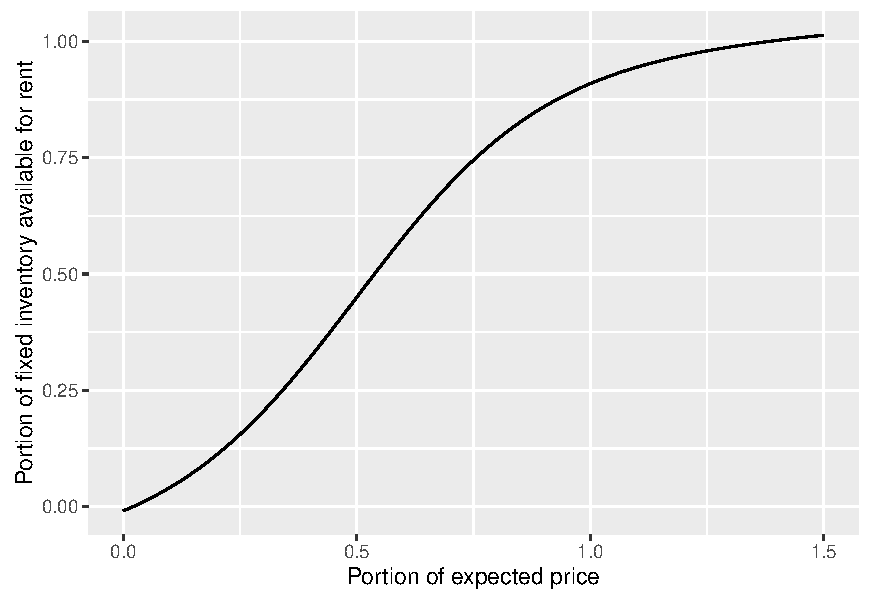
\includegraphics[scale=0.77]{aa/aa-floorspace-import-function}
\caption{Floorspace import function}\label{fig:aa-floorspace-import}
\end{figure}

The following floorspace-specific import equations are used in the AA import function(in place of the more general equations \ref{eq:6.22} through \ref{eq:6.24} used by all other imports found in \S\ref{sec:aa-import-export}):

\begin{equation}\label{eq:6.25}
PriceRef_c = \alpha_{Price, f} \times FLRPriceRef_f
\end{equation}
\begin{equation}\label{eq:6.26}
QRef_c = \alpha_{Qty,f} \times FLRQtyRef_f
\end{equation}
\begin{equation}\label{eq:6.27}
\Delta_c = \alpha_{\delta,f} \times FLRQtyRef_f
\end{equation}
\begin{equation}\label{eq:6.28}
\eta_c = \alpha_{\eta,f} / FLRPriceRef_f
\end{equation}
\begin{equation}\label{eq:6.29}
\mu_c = (\alpha_{\lambda,f} / FLRPriceRef_f) \cdot FLRQtyRef_f
\end{equation}
\noindent where:
\begin{align*}
f &= \text{index of floorspace categories} \\
FLRPriceRef_f &= \text{commodity-specific annual price (\$/Msqft) for (imported) floorspace} \\
 &~~~~~\text{(also used as a starting price for zones with no starting price)} \\
FLRQtyRef_f &= \text{current year quantity of (imported) floorspace of type $f$} \\
\alpha_{Price,f}, \alpha_{*,f} &= \text{floorspace-specific parameters to be adjusted in calibration}
\end{align*}

\subsection{Equilibrium Solution and Convergence Criteria}

The quantities of each commodity being bought and sold in each exchange zone by the activities in the model area (not imports or exports) are calculated as a sum of the buying and selling quantities solved for in the AA ``middle'' technology model (see \S\ref{sec:aa-pca-technology}), as follows:
\begin{equation}\label{eq:6.30}
TBD_{c,k} = \sum_{z \in Z} B_{c,z,k}
\end{equation}
\begin{equation}\label{eq:6.31}
TSD_{c,k} = \sum_{z \in Z} S_{c,k,z}
\end{equation}
\noindent where:
\begin{align*}
c &= \text{index of commodity} \\
k, z &= \text{index of zones, when paired indicate origin, destination zone} \\
Z &= \text{set of all model zones} \\
B_{c,z,k} &= \text{quantity of commodity $c$ consumed in zone $z$ that is allocated to} \\
 &~~~~~\text{(come from) exchange location $k$ (Buying\_\$commodity.zmx [equation \ref{eq:6.16}])} \\
S_{c,k,z} &= \text{quantity of commodity $c$ produced in zone $z$ that is allocated to (go to} \\
 &~~~~~\text{exchange location $k$ (Selling\_\$commodity.zmx (equation \ref{eq:6.12})} \\
TBD_{c,k} &= \text{total quantity of commodity $c$ being bought in exchange zone $k$ by all} \\
 &~~~~~\text{activities in the model area (ExchangeResults[InternalBought])} \\
TSD_{c,k} &= \text{total quantity of commodity $c$ being sold in exchange zone $k$ by all activities in} \\
 &~~~~~\text{the model area (ExchangeResults[InternalSold])}
\end{align*}

The quantities of each commodity being bought and sold in each exchange zone in total (by the activities in the model area as well as imports and exports) --- also called the aggregate demand and aggregate supply for commodity $c$ in exchange zone $k$ --- are calculated as follows:
\begin{equation}\label{eq:6.32}
TDem_{c,k} = Q_{c,e,k} + \sum_{z \in Z} B_{c,z,k}
\end{equation}
\begin{equation}\label{eq:6.33}
TSup_{c,k} = Q_{c,i,k} + \sum_{z \in Z} S_{c,k,z}
\end{equation}
\noindent where:
\begin{align*}
TDem_{c,k} &= \text{aggregate demand for commodity $c$ in exchange zone $k$ by all activities} \\
 &~~~~~\text{in the model area} \\ 
TSup c,k &= \text{aggregate supply for commodity $c$ in exchange zone $k$ by all activities} \\ 
 &~~~~~\text{in the model area} \\ 
Q_{c,i,k} &= \text{quantity of commodity $c$ imported to exchange location $k$} \\
Q_{c,e,k} &= \text{quantity of commodity $c$ exported from exchange location $k$} 
\end{align*}

At convergence these bought and sold amounts in a given zone, $TDem_{c,k}$  and $TSup_{c,k}$ are equal. This amount is also the referred to as the ``exchange quantity'' for the commodity in the zone:
\begin{equation}\label{eq:6.34}
TE_{c,k} = TDem_{c,k} = TSup_{c,k}
\end{equation}
\noindent where $TE_{c,k}$ is the exchange quantity for commodity $c$ in exchange zone $k$. 

Since AA solves the system using numerical methods, equation \ref{eq:6.34} is not solved exactly, but within a certain convergence tolerance. The residual commodity amount, $TSup_{c,k} - TDem_{c,k}$ is reported as output to allow user checks for appropriate convergence tolerance (ExchangeResults[Surplus]).

\subsubsection{Managing and Monitoring the Solution Algorithm}
The AA Module searches for the set of prices that establishes the equilibrium solution where all the markets clear, where the total demand minus the total supply minus the total demand for each commodity $c$ in each exchange zone $k$, denoted $Residual_{c,k}$, is zero. It performs this search in a series of iterations.

In each iteration a new set of prices is considered. The extent that the values for $Residual_{c,k}$ are not zero with these prices is evaluated and appropriate updates to these prices are calculated and applied. The process then moves to the next iteration with these prices used as the new set of prices.

This search process is managed by specifying the criteria that must be satisfied in order for the process to stop and by controlling elements of the calculation of the updates to prices in each iteration. These elements of this management are outlined below.

\subsubsection{Measuring Extent of Convergence and Specifying Stopping Rules}
In each iteration, the search process measures the extent that the values for $Residual_{c,k}$are not zero using a weighted sum-of-squares value as follows:
\begin{equation}\label{eq:6.35}
MClear = \sum_{c \in C} VergeWt_c^2 \sum_{k \in K} (Residual_{c,k})^2
\end{equation}
\noindent where:
\begin{align*}
MClear &= \text{residual-squared measure of the extent that all markets have not cleared and} \\
 &~~~~~\text{the condition that $Residual_{c,k} = 0$ for all $c$ and $k$ has not been satisfied;} \\
 &~~~~~\text{a value of 0 indicates the condition has been fully satisfied} \\
VergeW_{tc} &= \text{weight applied to residual-squared values for commodity $c$ to account for} \\
 &~~~~~~\text{units effects when summing residual-squared values across commodities} 
\end{align*}

The search process uses this value in its determination of the appropriate update to the prices for the next iteration.

The search process reports the value of $MClear$ in each iteration, by writing it to the log file. This value is influenced by the units used for the commodities and by the size of the markets considered, which can make it difficult to interpret.  A normalized form of the measure is also calculated and reported as follows:
\begin{equation}\label{eq:6.36}
TClear = \left[ \sum_{c \in C} VergeWt_c^2 \sum_{k \in K} (Residual_{c,k})^2 \right]^{0.5} /  AveExchgTotal
\end{equation}
\noindent with:
\begin{equation}\label{eq:6.37}
AveExchgTotal = \left[ \sum_{c \in C} VergeWt_c^2 \sum_{k \in K} (0.5 \cdot (TSup_{c,k} +TDem_{c,k}))^2 \right]^{0.5}
\end{equation}
\noindent where $TClear$ is the normalized measure of the extent that all markets have not cleared and the condition that $Residual_{c,k}$ = 0 for all $c$ and $k$ has not been satisfied; a value of zero indicates the condition has been fully satisfied (in software: GOF output to logfile).

$TClear$ may be much larger than 1.0 in the initial iterations of a search, but will quickly drop to much smaller values on its way to a value of zero when the search process is converging to a solution.

The search process is terminated when either (a) the values for $Residual_{c,k}$ satisfy specified convergence criteria indicating they are sufficiently close to zero, or (b) the specified maximum number of iterations is reached.

The maximum number of iterations, $Imax$, is specified in the aa.properties Run Control file using the setting for aa.maxiterations. The number of iterations required for the AA Module to converge is influenced by many factors, so it is not possible to provide definitive guidance on suitable values for $IMax$ overall. That said, in general, with convergence criteria that are reasonable and not too stringent and starting prices are not too wildly different from the solution prices, it should not take more than about 500 iterations for the AA Module to converge. Numbers of iterations well beyond that without convergence may be indicative of problems making it too difficult (and perhaps even impossible) to achieve convergence.

Two basic types of convergence criteria regarding the values for $Residual_{c,k}$are included. Both use normalized measures that are always positive and are zero at the equilibrium solution. One concerns the extent that all markets are cleared, the other concerns the extent that individual markets are cleared. Each is described below:

\subsubsection{(a) Total Clearance Criterion}
The ``total clearance'' criterion concerns the extent of market clearance for all commodities in all markets altogether, and uses the $TClear$ measure defined above. A maximum value is specified and $TClear$ must be less that this maximum value in order for the criterion to be satisfied. This maximum value is denoted $MaxTClear$, and it is specified in the aa.properties Run Control file using the setting for aa.maxTotalClearance.

In general, values of $MaxTClear$ in the range of 0.001 are used.

Further guidance on appropriate values for $MaxTClear$ can be obtained by considering the values for $MClear$ and $AveExchgTotal$ arising in a typical economy with specific total differences between supply and demand in the units being used. For example, if the units are dollars for all commodity values and all the commodity weights $VergeWtc$ are 1.0, then a combined residual of about 1000 dollars for all commodities in all zones (a comparatively small amount in most cases) would result in a value of $MClear$ of about 1e6. With a total economy of 10 billion dollars of exchanges, the value of $AveExchgTotal$ is 1e10, so the resulting value of $TClear$ is 1e-7.

The search algorithm reports the value of $TClear$ in each iteration, making it possible to monitor the progress towards satisfying the requirement that $TClear$ be less than $MaxTClear$.

\subsubsection{(b) ``Specific Clearance'' Criterion}
The ``Specific Clearance'' criterion concerns the extent of clearance for specific commodities in individual markets. It uses a measure for an individual commodity and market as follows:
\begin{equation}\label{eq:6.38}
SClear_{c,k} = | Residual_{c,k} | / SingleExchgTotal_{c,k}
\end{equation}
\noindent with:
\begin{equation}\label{eq:6.39}
SingleExchgTotal_{c,k} = | (0.5 \cdot (TSup_{c,k} +TDem_{c,k})) | + ConFac \cdot AveExchgTotal / VergeWt_c
\end{equation}
\noindent where $ConFac$ is a factor adjusting the scaled contribution to the denominator ensuring it is not zero in $SClear_{c,k}$ (in software: GOF output to logfile). A maximum value is specified and all $SClear_{c,k}$ for all $c$ and $k$ must be less than this maximum value in order for the criterion to be satisfied. This maximum value is denoted MaxSClear, and it is specified in the aa.properties Run Control file using the setting for aa.maxSpecificClearance.

In general, values of $MaxSClear$ in the range of 0.01 are used.

The value for $ConFac$ is specified in the aa.properties Run Control file using the setting for aa.contributionfactorscale. In general, a value approximately equal to the reciprocal of the number of LUZ in the model is used.

Certain $SClear$ values may be much larger than 1.0 in the initial iterations of a model run, but will quickly drop to much smaller values on their way to values of zero when the model is converging to a solution.

The search algorithm reports the maximum value of $SClear_{c,k}$ for each commodity $c$ across the set of exchange zones $k$ in each iteration, making it possible to monitor the progress towards satisfying the requirement that all the $SClear_{c,k}$ be less than $MaxSClear$.

\subsubsection{Controlling Price Update Calculation}
The updates to the prices in a given iteration are calculated seeking to minimize the value of $MClear$.

These updates to the prices are calculated by first calculating initial ``full update'' values that are then multiplied by a step size value in order to get the values that are applied in the iteration.

The initial ``full update'' in the price for each commodity in each exchange zone is the sum of (a) an adjustment calculated for an average price across all exchange zones and (b) an adjustment calculated for the local price for just that exchange zone multiplied by the a weighting factor called the Local Step Size Adjustment factor, or $StepLoc$.

The value for $StepLoc$ used in this calculation is specified in the aa.properties Run Control file using the setting for aa.localPriceStepSizeAdjustment. It can be used to adjust the relative contribution of average price change using an exact Newton's method and the local price change using a local derivative.

In general, a value of 0.5 is used for $StepLoc$.

The initial ``full update'' values obtained as described above are then multiplied by the Full Step Size Adjustment factor, Step, in order to get the ``adjusted update'' values used in the iteration.

If these adjusted update values result in a lower (better) value for $MClear$, then the software automatically increases the value of Step slightly for the next iteration. Further such increases in Step will be made, if appropriate, in subsequent iterations until a specified maximum value for Step is reached.  The search process will continue with this maximum value for Step being used as long as lower values for $MClear$ are being obtained.  If these adjusted update values results in a higher (poorer) value for $MClear$, then these values are not applied and the value of Step is reduced, and a new and smaller value of Step is used to calculate new adjusted update values to replace the abandoned ones. Further reductions to Step will be made, if required, until it reaches a specified minimum value. Iterations will continue with this minimum value until lower values for $MClear$ are being obtained.

The initial, maximum and minimum values for Step --- StepInit, StepMax and StepMin, respectively --- are specified in the aa.properties Run Control file using the settings for aa.initialStepSize, aa.maximumStepSize and aa.minimumStepSize, respectively. 

Regardless of these settings, if the current value of Step results in a numerical overflow, the value of Step is reduced even if doing so would result in it being below the specified minimum value.

A low value for StepInit, around 0.001, is appropriate, particularly in the initial stages of model development where there are larger changes being made and the starting prices are less likely to be close to the solution prices.  This allows the solution algorithm to establish an appropriate search direction before moving too much at the start.

The value for StepMin is the minimum value of Step the search process can use when encountering increases rather than decreases in $MClear$.  When the search process has been forced to use StepMin, it is still moving the direction the derivatives have indicated is the most appropriate, but is reducing the amount that it is moving because it has found that the result is not good when it moves a larger amount.  Sometimes the search process has to get ``over a hump'' before it can proceed to even lower values in the $MClear$ measure of convergence.  It will do this using the minimum value for Step.  If this minimum value is too small, then it will take a large number of iterations to get ``over the hump'', requiring large quantities of computer runtime. But the search process uses the derivatives at its current location to establish an indication of the most appropriate direction for the next iteration, and if the minimum value for Step is too large, then the solution algorithm may not be able to keep from moving beyond the range where this indication is accurate, and may then jump around ``wildly'' from one iteration to the next. A compromise value is required, usually established by trial and re-trial for each particular model. On the basis of experience a value of 0.01 for StepMin is a good place to start. 

The value for StepMax is the maximum value of Step the search process can use when encountering decreases in $MClear$. When the search process is using StepMax, it is making consistently good progress towards convergence. A value of 1.0 for Step results in the search algorithm using Newton's Method directly in the determination of the average price adjustment, which should lead to good convergence. A somewhat larger value for Step may further speed convergence. But, if a much larger value for Step is used, and the search process moves beyond the range where the indications provided by the derivatives at its current location are accurate, then the process may jump around ``wildly''. At that time, when it encounters an increase rather than a decrease in $MClear$, the algorithm will reduce the value of Step. An appropriate maximum value for Step can help avoid some of this increasing and decreasing of Step, and thereby help speed convergence. Finding an appropriate value is again a trial and re-trial process. Experience has shown that an effective strategy for helping minimize runtimes to convergence is to start with a value of 2.0 for the maximum value of Step, or even 2.0 divided by the value for the local price step size adjustment, and then keep reducing this value in subsequent model runs until there are comparatively few instances where Step is reduced from the maximum value.

At convergence, the AA model provides the following at the beta zone level prior to post-processing of some results to the alpha zone level (see \S\ref{sec:aa-p-processor}):
\begin{itemize}
\item Consistent (household and industry dollar) activity allocations by activity category by zone.
\item Commodity flow quantities from production zone to consumption zone via exchange zone.
\item Imports and exports by exchange zone.
\item Exchange prices by commodity by exchange zone. 
\end{itemize}

\subsection{P-Processor Integration}\label{sec:aa-p-processor}
To facilitate AA's interaction with other SWIM2 modules, an AA p-processor is used to both create AA input files and post-process AA output files into the appropriate format. The AA pre-processor produces the following files used as working inputs to AA. These files pull data from other SWIM2 modules and previous year AA outputs:
\begin{itemize}
\item Current year modelwide activities in the ActivityTotalsW.csv[TotalAmount] field are culled from:
\begin{itemize}
\item A base file ActivityTotalsI.csv
\item SPG1 module household counts:householdsByHHCategory.csv [spg1Households]. 
\item NED module modelwide industry/institution production activity in activity\_forecast.csv[output], government\_forecast.csv.
\item NED module modelwide imports and exports for goods commodities in trade\_forecast.csv.
\item Amount of office support activity is calculated based on the use of the office support commodities by the associated production activities. The base file TechnologyOptionsI.csv is read to determine the use rates; these are multiplied by the size of the production activities to determine total use, and divided by make rate (usually 1.0) to determine required industry size.
\end{itemize}
In the first AA run, only the NED updates and the office support update happen; households and imports/exports are read directly from the base ActivityTotalsI.csv file.

\item Current year fixed floorspace inventory in FloorspaceW.csv file, updates the current year ALD module floorspace output FloorspaceI.csv with fixed production-based quantities of agriculture and forest lands (in acres) found in the AgForestFloorspace.csv.
\item Zone-specific size terms ActivitiesZonalValuesW.csv come from:
\begin{itemize}
\item A base file ActivitiesZonalValuesI.csv if provided, otherwise the previous year zonal activity output ActivityLocations.csv[Quantity]
\item ALD output current year construction activity Increments.csv[IncMSQFT]
\end{itemize}
\item Current year technical coefficients in TechnologyOptionsW.csv are adjusted from base file TechnologyOptionsI.csv with adjustments made to industry labor use. Industry labor use rates are scaled based on the SPG to NED HHs per employees, relative to the 2009 reference year ratios (found in GlobalTemplate.properties [aa.09.productivity.rate]).
\end{itemize}

In addition to the preprocessor steps, a Python file (retexchange.py) runs before AA. This script updates ExchangeImportExportI.csv with size terms for exchange locations for commodities of the `a' type (can be exchanged in any zone). The size terms are determined based on the amount of space available for conducting the exchange (Warehouse or Retail), according to the input file ExchangeSizeTermTypes.csv.

Selected AA outputs (Table \ref{tab:aa-outputs}) are also disaggregated to the alpha zone level by the AA post-processor for use in other SWIM2 modules. Several of these AA post-processor activities are detailed below.

\subsubsection{Alpha Zone Activity and Commodity Totals}
AA works at the beta zone level and allocates modelwide activity to beta zones. The AA post-processor knows the distribution of floorspace by alpha zone from the ALD module. By assuming that, at the disaggregate level, individual units of an activity (e.g., the space required for an individual worker) only use a single floorspace type, the AA output beta zone activity totals can be allocated to alpha zones. The following formulation is used to produce alpha zone activity levels [ActivityLocations2.csv]:\footnote{A similar process is used to develop alpha zone commodity quantities (in binary and comma-separated value formats) [FloorspaceZoneTotalMakeUse.csv]. However, this file has not been fully debugged and should not be used.}
\begin{equation}\label{eq:6.40}
W_{a,\alpha} = W_{a,z} \cdot \sum_{f \in F} \left[ U_{f,a,z} / \sum_{f1 \in F} U_{f1,a,z} \right] \cdot FLR_{f,\alpha} / \sum_{\alpha 1 \in Z} FLR_{f, \alpha 1}
\end{equation}
where:
\begin{align*}
W_{a,\alpha} &= \text{amount of activity $a$ in alpha zone $\alpha$ (ActivityLocations2.csv[Quantity])} \\
W_{a,z} &= \text{amount of activity $a$ in beta zone $z$ (ActivityLocations.csv[Quantity])} \\
U_{f,a,z} &= \text{amount of floorspace commodity $f$ consumed per unit of activity $a$ in} \\
 &~~~~~~\text{beta zone $z$ (MakeUseW[marginal] and [discretionary]} \\
F &= \text{set of floorspace types used by activity $a$ in beta zone $z$} \\
FLR_{f,\alpha} &= \text{amount of floorspace type $f$ in $\alpha$ (FloorspaceW.csv[BldgMSQFT])} \\
\alpha 1 \in z &= \text{set of alpha zones located in beta zone $z$ (FloorspaceZonesI.csv)} 
\end{align*}


\subsubsection{Labor Flow Marginals}
In other SWIM2 modules, AA labor flows at the beta zone are used to assign home location (SPG2) and workplace (PT). The flows are expanded to alpha zone flows in the respective modules using AA-generated alpha zone labor flow marginals. These marginals are generated by the AA post-processor essentially expanding the AA beta zone labor production (at the home end) and consumption (at the workplace end) vectors to alpha zones. To do so, AA first expands the overall activity values into alpha zones (equation \ref{eq:6.35} forActivityLocations2.csv) and then applies the AA output technical coefficients (MakeUseW.csv) to these values. The technical coefficients are assumed to be equivalent for all alpha zones within a beta zone. The results are used in the PT module's Workplace Location Choice model (LaborDollarProductionSum.csv and LaborDollarConsumptionSum.csv by occupation and household category) and SPG2 module's Household Home Zone Assignment module (LaborDollarProduction.csv, LaborDollarConsumption.csv by occupation) in the current year. Labor consumption is summed across occupation and industry categories while labor production is summed across occupation and household categories. The ``sum'' versions of the files used by PT, are only categorized by occupation for production and consumption.

\subsubsection{Scaled Labor Use Coefficients}
Due to social and technological changes between 1990 and 2000, labor production per household has increased since 1990 inputs (e.g., increased women participation in the workforce), while labor consumption per industry activity (e.g., rising labor productivity) decreased. To address this net effect in the AA module, the initially assumed fixed labor use coefficients, are dynamically scaled relative to a 1998 base year productivity (source of initial IMPLAN-based make and use technical coefficients).This requires calculating a current year productivity (jobs/million dollars) from current year NED workers by industry and industry output dollars (activity\_forecast.csv).This current year productivity (jobs/million dollars) is divided by the fixed 2009 productivity rate (0.121037363 jobs/Activity, in millions of dollars, found in GlobalTemplate.properties [aa.09.productivity.rate]) to calculate the current year ``LaborUseScaling factor''. This scaling factor is applied to the TechnologyOptionsI.csv file use coefficient for all labor occupations ([Minimum] and [Discretionary] fields) and stored in the working TechnologyOptionsW.csv file used in the current year AA run. 

\section{Software Implementation}
As an equilibrium model, AA must find a mathematical solution. The exchange zones simulate markets where the aggregate supply (the sum of the selling allocations together with the quantity of imports, both elastic with respect to the exchange price in equation \ref{eq:6.32} for demand and \ref{eq:6.33} for supply) meets the aggregate demand (the sum of the buying allocations together with the quantity of exports). The AA module numerically solves for the equilibrium solution, adjusting the exchange prices in the exchange locations until all the markets clear, that is, where $TDem_{c,k} = TSup_{c,k}$ within a specified tolerance or convergence criteria (set in the 
globalTemplate.properties file).

The search algorithm calculates the partial derivative of the total surplus demand (excess of demand by buyers and exporters over supply by sellers and importers) in each exchange zone with respect to the price in that exchange zone, repeating this for all commodities in all exchange zones. The derivatives with respect to prices in other zones or for other commodities are assumed to be zero and a price change is calculated. A step adjustment factor is applied to the step to speed and aid convergence. If a step results in a lower aggregate sum-of-squares surplus demand, then the step adjustment factor is increased slightly for the next iteration. If a step results in a higher aggregate sum-of-squares surplus demand, then the step is abandoned, the step adjustment factor is reduced substantially and a new and smaller step is calculated to replace the abandoned one.

The AA module is implemented in Java, using the following main set of object classes:
\begin{itemize}
\item Activity type (AggregateActivity class).
\item Commodity type (Commodity class).
\item Set of make coefficients and associated formula indicating the byproduct production 
possibilities for an activity (ProductionFunction class).
\item Set of use coefficients and associated formula indicating the different production methods 
available for an activity (ConsumptionFunction class).
\item The amount of each activity in each zone(AmountInZone class).
\item The tracking of the amounts of commodities bought, sold, imported and exported in each 
exchange (Exchange class).
\item The logit model to allocate the commodities bought by a zone (i.e. produced within a 
zone) amongst the available exchanges (BuyingZUtility class).
\item The logit model to allocate the commodities sold to a zone (i.e. consumed within a zone) 
from amongst the available exchanges (SellingZUtility class).
\item Tracking each of the flows between production and consumption points and the 
exchanges (CommodityFlowArray class).
\item Each zone (AbstractTAZ and alpha zone classes).
\item The formula for the imports and exports in each zone (LogisticPlusLinearFunction class).
\item The calculation of the transport disutility from the matrix of travel times and distances 
(TimeAndDistanceTravelUtilityCalculator class).
\end{itemize}

The software process for each iteration of the search procedure involves requesting that each AggregateActivity class allocate the total region-wide quantity of activity (from NED and SPG modules) to the various AmountInZone classes (``highest'' level AA location allocation model); the AmountInZone classes are used to report the composite utility of locating in each zone. The AmountInZone class in turn allocates the production and consumption quantities of commodities using the ProductionFunction and ConsumptionFunction classes (``middle'' level AA technology choice module); the ProductionFunction and ConsumptionFunction classes are used to report the utility of consuming and producing in the zone (used by the ``highest'' level AA module). The BuyingZUtility class and SellingZUtility class allocate the resulting commodities bought and sold by an activity in a zone to amongst the exchanges, updating the flows in the CommodityFlowArray (``lower'' level AA transport-related allocation model).

The lowest level of this chain of allocations is the most computationally intensive. Once the prices are established at the beginning of the iteration, the ``lowest'' level model uses the BuyingZUtility and SellingZUtility classes to calculate the Buy and Sell composite utilities of equations \ref{eq:6.14} and \ref{eq:6.18} repeatedly during an iteration. Since these composite utilities do not change as long as the prices are not changing, these values are cached during an iteration and second and subsequent requests for the same composite utility value during an iteration return the previously computed value.

The AA module runs on a single machine or it can be distributed across multiple machines. When distributed, the ``lowest'' level allocations of buying and selling locations for commodities consumed or produced in a zone (BuyingZUtility and SellingZUtility classes) are farmed out to various machines by a master process. If the module is run on a single machine different processor cores are used for different Activities and Commodities and these cores can communicate through shared memory instead of over the network. Single powerful machines with many cores can usually run AA faster than many machines because of the lower communication overhead.

In each iteration of the search algorithm first the calculations of $CUSell$ and $CUBuy$ (``lowest'' level allocation model) are distributed, with each work task being the calculation of the set of $CUSell$ and $CUBuy$ for all zones for a single commodity. Later in the same iteration the allocation of amounts bought and sold to exchange zones (``middle'' level technology choice) is distributed, with each work task being the allocation of the amounts bought and sold in each consumption and production zone to the exchange zones for a single commodity. 

The following parameters are used to set the convergence criteria and control the constrained iteration process in AA ([globalTemplate.properties]):

{\small
\begin{verbatim}
    # Use these to control the AA runtime parameters
    aa.maxIterations=1000
    aa.initialStepSize = .001
    aa.minimumStepSize = .025 
    aa.maximumStepSize = 2.5
    aa.localPriceStepSizeAdjustment = 1
    aa.maxTotalClearance=0.00005
    aa.maxSpecificClearance=0.02
    aa.ConFac=.01

    aa.constraint.iterations=2
    aa.constraint.smoothing=1.0
    aa.constraint.maxConstantChange=2.5
    aa.constraint.tolerance=0.02
\end{verbatim}
}

\section{S1 and S2 Module Parameters}
The AA module requires a number of parameters. These parameters are identified in the following sections as S1, S2 or S3 parameters, following the three-stage calibration approach in \S\ref{sec:calibration-approach} (page \pageref{sec:calibration-approach}). The specific process used to determine the chosen values for each parameter are indicated in the following sections. 

\subsection{Production Activity Allocation Parameters}\label{sec:pa-allocation-parameters}

Table \ref{tab:aa-p-activity-allocation} identifies the estimated parameters of the ``highest'' level AA production activity allocation module, discussed in \S\ref{sec:aa-pa-allocation-modelwide}. No ``other'' zonal attributes ($X_{v,k}$ in equation \ref{eq:6.02}) are currently specified.

%Table 6-1 AA Production Activity Allocation Parameters
\begin{table}
\centering
\caption{Production activity allocation parameters}\label{tab:aa-p-activity-allocation}
\begin{tabular}{l L{4.6in} c}
\hline
Parameter & Description & Level(s) \\
\hline
$\alpha_{size,a}$ & Utility function coefficient for the sensitivity to size & S1 \\
\gray $\alpha_{inertia,a}$ & Utility function coefficient for the sensitivity to the previous proportion of activity $a$ in zone $z$, representing inertia in allocation of activity $a$ & S3 \\
$InertiaConst_a$ & Coefficient modifying the sensitivity to the previous portion of activity $a$ in zones, that reduces the importance of the quantity when the previous quantity is small; ActivitiesI[InertiaTermConstant] & S3 \\
\gray $Constant_{a,z}$ & Utility function alternative specific constant for zone $z$ for allocation of activity $a$ & S2 \\
$\alpha_{prod,a}$ & Utility function coefficient for the sensitivity to composite utility associated with production technology for activity $a$ & S1/S3 \\
\gray $\delta_a$ & Utility function dispersion parameter for allocation of activity $a$ & S2 \\
\hline
\end{tabular}
\end{table}

The alternative zone-specific constants for the allocation of activity ($Constant_{a,z}$) are adjusted in the base year AA run to provide an exact match to observed base year distributions of employment, population and world-market import and export quantities. This process uses the AA constraint process to match zonal targets in ActivityConstraintsI.csv with constants output in activityLocations.csv. 

Several coefficients allow sensitivity to composite utility associated with production and consumption technology ($\alpha_{prod}$) in the ``highest'' level activity allocation utility function. During calibration, the values shown in Table \ref{tab:aa-pc-activities} were established. The Substitution Nesting parameter values are dependent upon the LocationDispersionParameters.

\begin{table}    % Table 6-2
\centering
\caption{Production and consumption activity allocation parameters}
\label{tab:aa-pc-activities}
\begin{threeparttable}
\begin{tabular}{l *{6}{c}}
\hline
\multirow{2}{*}{Activity categories\tnote{a}} & \multirow{2}{*}{$\lambda_a$} & \multirow{2}{*}{$\alpha_{size}$\tnote{b}} & \multirow{2}{*}{$\alpha_{inertia}$} & Inertia & \multicolumn{2}{c}{Technology coefficients} \\
\cline{6-7}
 & & & & $Const_a$ & $\lambda_{m,a}$ & $\alpha_{prod,a}$ \\ 
\hline
Industry & Calibrated values & 1 & 1 & 1 & Calibrated values & 1 \\
\gray Households & Calibrated values & 1 & 1 & 1 & Calibrated values & 1 \\
Institutions & Calibrated values & 1 & 1 & 1 & Calibrated values & 1 \\
\gray SCTG importers \& exporters & 1 & 1 & 1 & 1 & 1 & 1 \\
\hline
\end{tabular}
\begin{tablenotes}
\footnotesize
\item[a] $U_{nmcis}$ true for all but importers, exporters, and institutions with calibrated utility values. $U_{nmp}$ is false for all activities with utility value of -100.
\item[b] $\alpha_{size}$ is the size term coefficient, which is a S1 parameter (see \S\ref{sec:ned-s1-s2}).
\end{tablenotes}
\end{threeparttable}
\end{table}

Several dispersion activity allocation parameters are S2 parameters. They include the dispersion parameter for the allocation of activity ($\lambda_a$) in the production activity allocation utility function and additional dispersion parameter for the allocation of by-product and input substitutes made by each activity ($\lambda_{m,a}, \lambda{u,a}$) in the production and consumption allocation utility functions. The coefficients of inertia, $\alpha_{inertia}$, in production allocation activity reflects the sensitivity to the previous proportion of each activity in each zone are currently set to zero. $U_{nmc}$ and $U_{nmp}$ affect the ability of activities to produce and consume less or more of commodities without substituting production and consumption to other modeled commodities.

\subsection{Production and Consumption Allocation Parameters (Technology)}\label{sec:aa-pc-allocation}

The estimated parameters of the AA production activity allocation module, discussed in \S\ref{sec:aa-pca-technology}, are shown in Table \ref{tab:aa-pc-allocation}. The dispersion parameters values are shown previously in Table \ref{tab:aa-pc-activities}. The values of the other listed parameters are discussed in the remainder of this section.

\begin{table}
\centering
\caption{Production and consumption allocation parameters}\label{tab:aa-pc-allocation}
\begin{tabular}{l L{4.9in} c}
\hline
Parameter & Description & Level(s) \\
\hline
$\delta_{m,a}$ & Utility function dispersion parameter for allocation of technology for activity $a$ & S2, S3 \\
\gray $M_{c,a,p}$ & Make technical coefficient for commodity $c$ produced by activity $a$ under technology option $p$ & S1 \\
$U_{c,a,p}$ & Use technical coefficient for commodity $c$ used by activity $a$ under technology option $p$ & S1 \\
\hline
\end{tabular}
\end{table}

\subsubsection{Aggregate Economic Flows Table}
The 2009 IMPLAN system, which has a Social Accounting Matrix (SAM), was used to obtain indications of the relationships between households and industries. The Census PUMS was used to obtain further details about households. The IMPLAN  and Census data were processed and combined  to build an ``aggregate economic flows'' table, which is similar in structure to the design diagram but has quantity information to show the size of each interaction in aggregate across the study region. The processing used an Oregon-specific PostgresSQL database, which uses standard SQL (structured query language) syntax.\footnote{The HBA Specto Oregon PostgresSQL database and ``Preparing Aggregate Economic Flows Table'' documentation, submitted to ODOT as part of TLUMIP4 WOC19 AA update (November 2011), can be accessed from \url{https://projects.hbaspecto.com/groups/buildingapecasmodel/wiki/cc0ef/Task_21_Aggregate_Economic_Flows.html}.} The scripts in the database establish the make and use coefficients for the normal technology options in PECAS. some of the details of these scripts are described below however the separate document should be consulted for specifics.  

%Table 6-3 AA Production and Consumption Allocation Parameters

\subsubsection{Fixed Make Technical Coefficients data preparation}
Make and Use tables from the 2009 IMPLAN Social Accounting Matrix (SAM) were obtained for the study region (Oregon statewide and Halo counties). Make coefficients are also called ``by-product coefficients,'' and use coefficients are also called ``absorption coefficients.'' The Oregon-specific PostgresSQL database was used to develop these coefficients. [56]

Within the SAM, modelwide make and use tables identify the dollar value of both domestic and foreign, production and consumption of various commodities, by both industry and institutions. An additional Use of Factors table provides the dollar amount of factors used by each industry. The ``employment compensation'' factor was called out specifically in AA as labor wages. Other IMPLAN factors (i.e., Proprietary Income, Other Property Income, Indirect Business Taxes) were dispersed among the various industries. [12] 

AA models goods flows (in units of 2009 dollars) rather than money flows found in IMPLAN input-output table. In an input-output table, the ultimate purchaser of a commodity is assumed to purchase the commodity itself from its producer and, if wholesale and/or retail trade were involved, to purchase only the wholesale and retail margins from the trade sectors. This allows an input-output model to reflect changes in the quantity demanded of a particular commodity in the production of that commodity. This essentially imposes a distribution system on the flow of goods, by consolidating various ``value added'' and margin components of a good's purchase price into a physically meaningful warehouse/retail distribution system with full value of the goods between each location, allowing correct translation into goods movement.\footnote{Before de-margining, when a consumer purchases a good in IMPLAN, the purchase is represented as a payment for the raw good from the sector that produced it, plus the purchase of transport from the transport sectors and the purchase of trade margin (or markup) from the trade sectors. This accurately attributes the production component of different goods to the consumption of those goods, but does not represent the physical distribution system of goods.} To mimic the flow of goods, we set up exchange zones for certain goods sized based on the total amount of retail and wholesale space in the zone. The sellers of these goods transport them to these exchange zones using truck-based transport cost functions, and the buyers of these goods transport them to their homes. The following commodities received this treatment: 
\begin{quotation}
\noindent {SCTG04\_FKP\_FEED, SCTG05\_FKP\_FOOD\_meat, SCTG06\_FKP\_AGRI\_grain, \\ SCTG07\_FKP\_FOOD\_prep, SCTG08\_FKP\_FOOD\_alc, SCTG17\_PCC\_FUEL, \\
SCTG18\_PCC\_PETR\_oil, SCTG21\_PCC\_CHEM\_pharma, SCTG23\_PCC\_CHEM\_prod, \\
SCTG29\_PPP\_PAPR\_print, SCTG30\_OTH\_CLTH, SCTG36\_MIT\_TRAN, \\
SCTG39\_OTH\_FURN, SCTG40\_OTH\_MISC}
\end{quotation}

The household consumption of retail goods is thus represented by two flows in the PECAS model, as it is in IMPLAN.  One flow is based explicitly on the representation of retail sales and retail shopping trips with all the associated detail of home-to-shop trip making, and represents the purchases at retail establishments.  The other flow is more abstract, and will tend to be to the same zones as the first flow, but represents the flow of physical goods from the truck delivery point to the home.

The industries and commodities in the IMPLAN make table were aggregated into the industries and commodities used in AA. Most industries were then split into sub industries based on the types of floor space occupied. Some industries had their production space split between, for example, light industrial space and heavy industrial space. Several also were split to distinguishing line-production (e.g., factory floor) from management (in offices), reflecting their use of different floorspace types, important to correctly locating activity. The method to split these industries essentially involved:
\begin{enumerate}
\item Moving a portion of labor in each base industry to a new sector-specific office industry in the Make table, based on modelwide employment estimates (\S\ref{sec:aa-zonal-activity-targets});
\item Adding an equal amount of internal services/management to the use table of the base industry, representing the production industry's purchase of management services; and
\item Splitting the make and use of commodities between the production/office industries in proportion to their employment (shifting as much FIRE services to the office industry as possible).
\end{enumerate}
\noindent This required the following assumptions: constant average wages across floorspace types; constant labor productivity (2009 dollars worth of output produced per dollar of labor) across production floorspace types within unsplit industries; and constant production functions for the production industry portion across floorspace types The remainder of the industry's output was assigned to that industry in production space.

For industries with multiple types of production space, output in production space was split proportional to employment by detailed IMPLAN commodity. Each detailed IMPLAN commodity was assigned to one of the production space types. IMPLAN employee compensation was divided into household income-occupation groups based on US Census household income data (synthetic population). IMPLAN total compensation by industry was spread to occupations based on the distribution of employees by occupation within each industry. In future updates, this compensation distribution should be updated to take into account differences in average wage between occupations.

The resulting split make table was used to derive make coefficients for each combination of AA industry and commodity. A make coefficient represents the proportion of an industry's total output that is represented by a particular commodity. Make coefficients sum to 1.0 for any given industry.

\subsubsection{Fixed Use Technical Coefficients data preparation}
As with the make table data, use table data were derived from 2009 IMPLAN Social Accounting Matrix for the study area (Oregon plus Halo). Use coefficients are also called ``absorption coefficients.'' The IMPLAN use table was aggregated in the same manner as the make table. The Oregon-specific PostgresSQL database was used to develop these coefficients. [56] If an industry was split between multiple types of production space, use of inputs in production space was split proportional to employment by detailed IMPLAN industry. Each detailed IMPLAN industry was assigned to one of the production space types.

The resulting split use table was used to derive Use coefficients for each combination of AA industry and commodity. A use coefficient represents the proportion of an industry's total output that is represented by the use of a particular commodity. Industries use labor of various occupations and Internal Management Services are only consumed by associated industries. For example, ``Internal Services Resources'' commodity is consumed only by ``Resource-Ag and Mining'' and ``Resource-Forest.'' 

Similar to the previous version of AA (i.e., PI), it was found necessary to reallocation the consumption expenditures for education to households, rather than having government consume education. Tracking education dollars in the economy, households pay government through taxes for the consumption of education. A new commodity was added to reflect the amount of money given to education (K12 and Higher education) by IMPLAN government account (12002). This commodity is referred to as ``Education Reports to Sponsors'' Per [52] State and Local spending on K12-teaching in Oregon (\$4.679B) is 86.26 percent on overall education spending (\$5.425B). This includes spending of state and local tax revenues only, not tuition, private grants, or federal grants (which would reduce the K12 share to 85.57 percent, \$5.692B/\$6.652B). The IMPLAN government education account was split accordingly.

ACS PUMS 2005-2009 data were used in calculating the use of K12-teaching commodity by households. Number of K12 students in each household category was obtained from PUMS.

% Table 6-4 The use of K12-teaching commodity by each Household category was never referenced, so omitted

\subsubsection{Industry Technical Options data preparation}

The establishment of technology options for industry sets up an orthogonal set of options based on options for each commodity or commodity group that has elasticity in the model design. ``More'' and ``Less'' options are established so that the industry can choose to make or use more or less of the elastic commodities or commodity groups.  Labor was treated as a commodity group, so that industries can use more or less labor but not substitute different types of labor, whereas each space type was considered individually so that industries allowed to use more than one space type can switch between them as well as consume more or less space.  The generation of these options from the expected values in the Aggregate Economic Flows Table was performed by a script in the PostgreSQL database used to process the 2009 Oregon IMPLAN data. The script,pecas.build\_technical\_coefficient\_other\_options. is documented on the PECAS Wiki [55] \footnote{\url{http:/c62e8/Task_30_Identify_Technology_Options_Points_for_Each_Activity.html}}. The script itself is contained within the PostgreSQL database that has been delivered.

\subsubsection{Households Technical Clusters data preparation}
Technology options for each activity in PECAS model must be identified. In the case of household activities, the options represents a ``lifestyle,'' essentially the basket of goods and services consumed and produced by households of a specific income-size. The PUMS [Census Bureau, 2009] provides indications about how individual households of different types participate in the labor and housing markets, these data were used to establish household technology options in a clustering process.

Useful dimensions for clustering household choices that predispose daily activity patterns and travel behavior include residential location, labor force activity and auto-ownership. As currently specified in AA, a household's lifestyle cluster is defined by a combination of two sets of dimensions: space use (housing choice and quantity consumed) and household wage (produced).Because PECAS represents location choice elsewhere, location dimensions were not required in the cluster. Expenditure data, if available would be valuable addition to the process, albeit increasing the number of clusters. Using a two-step clustering algorithm as defined in reference [48], different household lifestyle clusters were identified for Oregon. The two-step clustering algorithm has two steps: (a) pre-cluster the cases into many small sub-clusters (b) cluster the sub-clusters resulting from pre-cluster step into a desired number of clusters.The first step calculates Bayesian information criterion (BIC) for each number of clusters within a specified range and uses it to find the initial estimate for the number of clusters. The second step refines the initial estimate by finding the greatest change in distance between the two closest clusters in each hierarchical clustering stage. The log-likelihood measure was used to calculate the distance between clusters. In general, larger households and higher income households have more variety in their labor force participation and housing consumption. These categories required more clusters to represent their flexibility to earn money and live in housing. Smaller and lower income households were more constrained in their choices, represented with less clusters.  

For Oregon, the lifestyle cluster dimensions are shown in Table \ref{tab:aa-household-lifestyles}. Floor space type is a categorical variable with 6 categories of residential space (previously defined in Table \ref{tab:floorspace-categories} on page \pageref{tab:floorspace-categories}), and the estimated square feet and wages are continues variables.  The clusters were chosen or split into sub-clusters so that each lifestyle clusters used only one space type. Table \ref{tab:aa-household-types} shows the number of households in the clustering sample. Figure \ref{fig:aa-lifestyle-clusters} shows the number of lifestyle cluster by each PECAS household type.

\begin{figure}
\centering
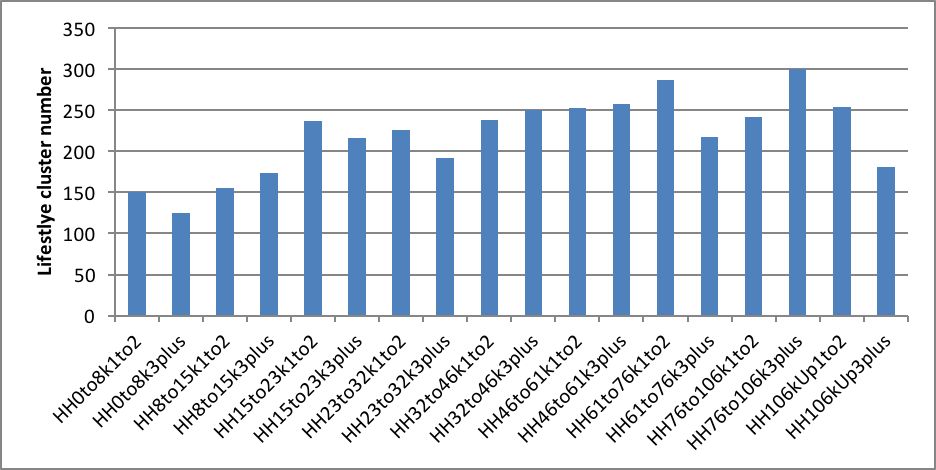
\includegraphics[scale=0.4, trim=0mm 2mm 0mm 0mm]{aa/lifestyle-clusters}
\caption{Lifestyle cluster numbers by Oregon AA household types}\label{fig:aa-lifestyle-clusters}
\end{figure}

\begin{table}     %Table 6-5 Dimensions of Oregon AA household lifestyle
\centering
\caption{Dimensions of Oregon AA household lifestyles}
\label{tab:aa-household-lifestyles}
\begin{tabular}{ccll}
\hline
Dimension & ID & Name & Type of variable \\
\hline
1 & 1 & Space type (6 categories) & Categorical \\
\gray  & 2 & Estimated square feet & Continuous \\
\hline
2 & 3 & Management and business worker's wage & Continuous \\
\gray  & 4 & Professional specialty worker's wage & Continuous \\
  & 5 & Education worker's wage & Continuous \\
\gray  & 6 & Health worker's wage & Continuous \\
  & 7 & Technical worker's wage & Continuous \\
\gray  & 8 & Sales and clerical professional worker's wage & Continuous \\
  & 9 & Sales and service labor worker's wage & Continuous \\
\gray  & 10 & Ag, Forest and Production specialty worker's wage & Continuous \\
  & 11 & Maintenance, construction, repair specialty worker's wage & Continuous \\
\gray  & 12 & Protective and transport specialty worker's wage & Continuous \\
  & 13 & Blue collar labor worker's wage & Continuous \\
\hline
\end{tabular}
\end{table}

\begin{table}     % Table 6-6 Oregon AA household type
\centering
\caption{Oregon AA household types}\label{tab:aa-household-types}
\begin{tabular}{clr}
\hline
Type ID & PECAS Household Type & N \\
\hline
1 & HH0to8k1to2 & 4,132 \\
\gray 2 & HH0to8k3plus & 767 \\
3 & HH8to15k1to2 & 4,031 \\
\gray 4 & HH8to15k3plus & 1,264 \\
5 & HH15to23k1to2 & 5,109 \\
\gray 6 & HH15to23k3plus & 2,089 \\
7 & HH23to32k1to2 & 6,428 \\
\gray 8 & HH23to32k3plus & 3,071 \\
9 & HH32to46k1to2 & 9,874 \\
\gray 10 & HH32to46k3plus & 5,477 \\
11 & HH46to61k1to2 & 8,977 \\
\gray 12 & HH46to61k3plus & 6,150 \\
13 & HH61to76k1to2 & 6,690 \\
\gray 14 & HH61to76k3plus & 5,910 \\
15 & HH76to106k1to2 & 8,166 \\
\gray 16 & HH76to106k3plus & 8,626 \\
17 & HH106kUp1to2 & 8,361 \\
\gray 18 & HH106kUp3plus & 9,610 \\
\hline
\end{tabular}
\end{table}

\subsection{Buying and Selling Allocation Parameters}
Table \ref{tab:bs-allocation-parameters} identifies the estimated parameters of the AA buying and selling allocation module, discussed in \S\ref{sec:aa-pca-technology}. The values of the parameters are discussed in the remainder of this section.

% Table 6-5 AA Buying and Selling Allocation Parameters
\begin{table}
\centering
\caption{Buying and selling allocation parameters}\label{tab:bs-allocation-parameters}
\begin{tabular}{lp{4.8in}c}
\hline
Parameter & Description & Level \\
\hline
$\delta_{size,s}$ & Utility function coefficient for the sensitivity to size & S1 \\
\gray $\delta_{size,b}$ & Utility function coefficient for the sensitivity to size & S1 \\
$\delta_{price,s}$ & Utility function coefficient for the sensitivity to price when selling & S1 \\
\gray $\delta_{price,b}$ & Utility function coefficient for the sensitivity to price when buying & S1 \\
$\delta_{tran,s}$ & Utility function coefficient for the sensitivity to transport utility & S2 \\
\gray $\delta_{tran,b}$ & Utility function coefficient for the sensitivity to transport utility & S2 \\
$\lambda_{s,c}$ & Utility function dispersion parameter for allocation of selling of commodity $c$ & S2 \\
\gray $\lambda_{b,c}$ & Utility function dispersion parameter for allocation of buying of commodity $c$ & S2 \\
$\phi_{s,c,a}$ & Factor adjustment to the composite utility of selling commodity $c$ by activity $a$ & S1/S2 \\
\gray $\phi_{b,c,a}$ & Factor adjustment to the composite utility of buying commodity $c$ by activity $a$ & S1/S2 \\
OptionWeight$_{p,a}$ & Weight of technology option $p$ for activity $a$ & S2 \\
\gray $\kappa_{c,dist}$ & Utility function coefficient for the sensitivity to trip distance when transporting a unit of commodity $c$ & S1 \\
$\kappa_{c,time}$ & Utility function coefficient for the sensitivity to trip travel time when transporting a unit of commodity $c$ & S1 \\
\gray $\kappa_{c,logsum}$ & Utility function coefficient for the sensitivity to trip mode choice composite utility when transporting a unit of commodity $c$ & S1 \\
\hline
\end{tabular}
\end{table}

\subsubsection{Buying and selling allocation parameters}
Buying and selling allocation S2 parameters include the dispersion parameter for allocation of buying and selling commodities ($\lambda_{s,c}, \lambda_{b,c}$), as well as the coefficients for the sensitivity to transport utility ($\delta_{tran,b}, \delta_{tran,s}$). The initial values for these parameters are shown in Table \ref{tab:aa-allocation-commodity}. Also shown is the exchange type assumed in the initial AA runs, which determines the location for the exchange. Floorspace is assumed non-transferable (n), while all other commodities are exchanged in any zone (a). Future runs may restrict non-floorspace exchanges to occur either in the production (p) or consumption (c) zone.

%Table 6-6 AA Buying and Selling Allocation Parameters by Commodity
\begin{table}
\centering
\caption{Buying and selling parameters by commodity}\label{tab:aa-allocation-commodity}
\begin{tabular}{lcccc}
\hline
\multirow{2}{*}{Parameter}& \multicolumn{4}{c}{Commodity categories} \\
\cline{2-5}
& Goods & Services & Labor & Floorspace \\
\hline
\multicolumn{5}{l}{\textit{Buying activity allocation coefficients}} \\
\gray Disperson parameter ($\lambda_{b,c}$) & Calibrated & Calibrated & Calibrated & 5  \\
Size coefficient ($\delta_{size,b}$) & 1 & 1 & 1 & 1 \\
\gray Price coefficient ($\delta_{price,b}$) & -1 & -1 & -1 & -1 \\
Transport coefficient ($\delta_{tran,b}$) & Figure \ref{fig:aa-vot} & Figure \ref{fig:aa-vot} & Figure \ref{fig:aa-vot} & 0  \\
\hline
\multicolumn{5}{l}{\textit{Selling activity allocation coefficients}} \\
\gray Disperson parameter ($\lambda_{s,c}$) & Calibrated & Calibrated & Calibrated & 5  \\
Size coefficient ($\delta_{size,s}$) & 1 & 1 & 1 & 1  \\
\gray Price coefficient ($\delta_{price,s}$) & 1 & 1 & 1 & 1  \\
Transport coefficient ($\delta_{tran,s}$) & Figure \ref{fig:aa-vot} & Figure \ref{fig:aa-vot} & Figure \ref{fig:aa-vot} & 0  \\
\hline
\multicolumn{5}{l}{\textit{Exchange type}} \\
& Mix of $p$ and $a$ & Mix of $p$ and $c$ & C & n  \\
\hline
\end{tabular}
\end{table}

For residential space, residential buying size terms are also used ($Size_{b,c,k}$ in equation \ref{eq:6.17}). These buying size terms are calculated as the quantity of space type $c$ in zone $k$ divided by the total of all residential space types in zone $k$. (All other buying size terms and selling size terms are left at their default value of 1.0).

Buying and selling composite utility includes allowance for factor and offset adjustments. All factor adjustments, $\phi_{s,c,a}$, are set to 1 and the offset adjustments, $USellRef_{c,a}$ and $UBuyRef_{c,a}$ are set to zero (Table \ref{tab:aa-household-lifestyles}). It is expected that in some cases, as calibration progresses, the factor adjustment may be set to 0 to completely remove the effect of individual buying and selling composite utilities on production utilities and thus on location utilities.

\subsubsection{Time and Cost Weights for Transporting Commodities}
Transport cost coefficients weigh the relative value of time and distance in the transport utility function. The AA transport function includes the overall sensitivity to transport ($\delta_{tran,b}$ and $\delta_{tran,s}$), as well as commodity-specific time and distance coefficients or commodity-specific coefficients on mode-choice logsums. 

The transport coefficient is essentially the inverse of the economic value per trip, allowing the time and distance parameters to be in units of cost per vehicle trip. These costs take into account variations in commodity value (labor or goods) and vehicle occupancy (tons or persons per vehicle). Goods transport costs are incurred at the production end (buying), while services (management and other) and labor transport costs are born at the consumption end (selling) of the exchange. Floorspace is non-transportable, so there are no transport costs (coefficients set to 1 or 0). These parameters are defined in the CommoditiesI.csv AA input file.

Freight commodity time and cost rates were calculated primarily with data from a 2000 WSDOT statewide modeling effort. In many cases, STCC commodity data was converted into the SCTG classification used in AA, weighted by 1999 IMPLAN production data (make value). These transport costs assume mode/vehicle operating costs and endogenized other cost, wage and mode split components. The transport coefficients are calculated as follows. Figure \ref{fig:aa-vot} shows the relationship assumed to calculate value of time for service-related trips. All monetary values have been converted into 2009 dollars. Note: In some cases final parameter values shown in Table \ref{tab:aa-transport-coefficients} were modified during calibration and do not follow these formula.

% Labeled as Table 6-7 Value of Time based on Wage Rate and Business Travel share of Trips, but actually a figure
\begin{figure}
\centering
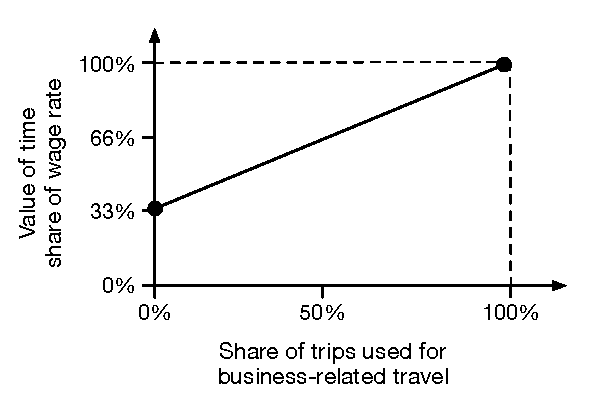
\includegraphics[scale=0.75]{aa/revised-vot-shares.pdf}
\caption{Value of time based upon wage rate and business travel share of trips}
\label{fig:aa-vot}
\end{figure}

\vspace{10pt}
\noindent For goods:
\begin{itemize}
\item $\delta_{tran,b}$ and $\delta_{tran,s}$ (trip/\$ of goods) = 1/(\$ payload value)
\item $\kappa_{c,time}$ (\$/vehicle-min) = (\$ per veh-hr) / (60min/hr) [user-input]
\item $\kappa_{c,dist}$ (\$/vehicle-mile) =  (\$ per ton-mile) * (Tons per vehicle) [user-input]
\item $\kappa_{c,logsum}$ (\$/mode choice utility) = 0
\end{itemize}

\noindent Which is based on assuming:
\begin{itemize}
\item 100 percent truck mode split [CT output (future)]
\item \$ payload value = \$ per ton*Tons per vehicle
\item \$ per vehicle-hr = \$20.42/Medium truck hour (other modes 0) [user-input]
\item \$ per ton-mile by mode = \$0.12 for MedTruck (\$.04 for Rail, \$3.71 for Air, \$0.01 for 
Barge) [user-input]
\item \$ per ton, ranging from \$18 to 90,691/Ton  (\$7,194/Ton average) 
\item Tons per vehicle: 9 to 22 tons/truck (average 15.6 tons/truck, 51 tons/railcar) [CT 
output (future)]
\end{itemize}

\noindent For labor/services:
\begin{itemize}
\item $\delta_{tran,b}$ and $\delta_{tran,s}$ (trip/\$ of production value) = (Trips per day) / (\$ of production value)

Labor: \$ of production value = (\$Economic wage per hour) * (8 hours/day)

Service: \$ of production value = (\$Annual Industry Use of Commodity) / (Annual vehicle trips) 
\item $\kappa_{c,time}$ = (\$Economic wage per hour)/(60min/hr): only for selected services
\item $\kappa_{c,dist}$ = (\$Operating cost per veh-mile)/(Auto occupancy): only for selected services
\item $\kappa_{c,logsum}$ = 1/\$ out-of-pocket (OPC) cost parameter for associated logsum (PT module 
estimated parameters): for all other services and labor/commute
\end{itemize}

\noindent Which is based on assuming:
\begin{itemize}
\item 100 percent auto mode split
\item Trips per day = 1 for labor commute trips, 1.5 for services (assuming some trip chaining)
\item \$ of production value per trip by purpose (for services) = \$Annual Total Use of 
Commodity/2009 Annual vehicle trips
\item \$ of production value per trip by purpose (for labor) = \$Economic wage per hour = 
(\$ Wage per hour) * (\%BusinessPurposeTrips * 67\% + 33\%)
\item \$ Wage per hour =  2005-2009 ACS PUMS wage data by occupation, where average calculated as annual wages divided by (weeks worked x hrs per week (WKHP)), limited to those working 49+ weeks/yr and not self-employed: \$3.74 to 21.98, average \$16.05 [AA data (future)]
\item \%BusinessPurposeTrips= 2009Modelwide IMPLAN share of total commodity used by industry = Annual IndustryUse/(Annual Household Use+Annual Institution Use]) [AA data (future)]
\item \$Annual Industry, Household, Institution, and Total Use of Commodity = 2009ModelwideIMPLAN data by trip purpose [AA data (future)]
\item 2009 Annual vehicle trips = 1994-1996 Oregon Travel Behavior Survey trips per HH by 
trip purpose * 2009 modelwide households
\item Auto Occupancy = 1994-1996 Oregon Travel Behavior Survey by trip purpose: 1.2 to 2.3, 
average 1.5 [user-input]
\item \$Operating cost per veh-mile = \$0.148/mile, consistent with PT module [user-input]
\end{itemize}

\subsubsection{Buying and selling price sensitivity coefficients}

The coefficients for the sensitivity to price when buying or selling ($\delta_{price,s}, \delta_{price,b}$), found in the buying and selling allocation utility functions, are set to 1 for all commodities, positive when selling and negative when buying. These are shown in Table \ref{tab:aa-transport-coefficients}. Thus, the utility function is in units of equivalent 2009 dollars.

% The transport coefficients table (Table 6-8 in original manuscript) is too large to fit in either landscape or portrait
% mode, even with footnote size text. So put in a placeholder for it, and we'll manually insert the oversized page in the
% final version of this document.
\begin{table}   % Placeholder
\centering
\caption{AA transport coefficients (per unit of production)}
\label{tab:aa-transport-coefficients}

\includegraphics[scale=0.5]{graphics/placeholder-female-superhero-c}
\end{table}
\begin{table*}
\centering

\includegraphics[scale=0.5]{graphics/placeholder-male-superhero-c}
\end{table*}

\subsection{Imports and Exports Model Parameters}
Table \ref{tab:aa-classic-parameters} identifies the estimated parameters of the classic style AA imports and exports model including floorspace imports, discussed in \S\ref{sec:aa-import-export} and \S\ref{sec:aa-floorspace-imports}. The values of the parameters are discussed in the remainder of this section.

% This combines what used to Tables 6-9 and 6-10, which appear to have the same header. Moreover, the latter was
% never referenced, so rather than lose the info it contained I simply put into bottom of this table.
\begin{table}
\centering
\caption{Classic-style AA imports and exports model parameters}
\label{tab:aa-classic-parameters}
\begin{tabular}{lL{4.9in}c}
\hline
Parameter & Description & Level \\
\hline 
$PriceRef_{c,i}$ & Reference price per unit for import of commodity $c$ & S1 \\
\gray $PriceRef_{c,e}$ & Reference price per unit for export of commodity $c$ & S1 \\
$QRef_{c,i}$ & Quantity of commodity $c$ imported to exchange location when the unit exchange price for commodity $c$ in exchange zone $k$ is at its import reference level $PriceRef_{c,i}$ & S1 \\
\gray $QRef_{c,e}$ & Quantity of commodity $c$ exported from exchange location when the unit exchange price for commodity $c$ in exchange zone $k$ is at its export reference level $PriceRef_{c,e}$ & S1 \\
$\gamma_{c,I}$ & Function coefficient for the rate of increase in imports of commodity $c$ for slope term & S1 \\
\gray $\gamma_{c,e}$ & Function coefficient for the rate of increase in exports of commodity $c$ for slope term & S1 \\
$\mu_{c,I}$ & Function coefficient for the rate of increase in imports of commodity $c$ for linear term & S1 \\
\gray $\mu_{c,e}$ & Function coefficient for the rate of increase in exports of commodity $c$ for linear term & S1 \\
$\eta_{c,I}$ & Function coefficient for sensitivity to difference in exchange price for commodity $c$ concerning increase in imports of commodity $c$ for exponent term & S1 \\
\gray $\eta_{c,e}$ & Function coefficient for sensitivity to difference in exchange price for commodity $c$ concerning increase in exports of commodity $c$ for exponent term & S1 \\
\hline
$F0Price$ & Reference price per unit of floorspace & S2 \\
\gray $PMidpoint$ & Quantity of floorspace supplied when the unit exchange price for floorspace in exchange zone $k$ is at its reference level $F0Price$ & S2 \\
$FDelta$ & Function coefficient for the rate of increase in imports of floorspace for slope term & S1 \\
\gray $FSlope$ & Function coefficient for the rate of increase in imports of floorspace for linear term & S2 \\
$FEta$ & Function coefficient for sensitivity to difference in exchange price for floorspace concerning the increase in floorspace supply for exponent term & S2 \\
\hline
\end{tabular}
\end{table}

In previous versions of the model, these parameters were critically important as they represented the appearance of imports and exports in the region. These import and export functions have been largely replaced by an explicit treatment of the flow of imports and exports to and from world-market zones to internal zones. The parameters in this table are now given appropriately small values to allow small amounts of imports to appear (and exports to disappear) in individual zones in cases where small imports or exports are necessary to balance supply and demand but quantities are irrelevant for transportation planning purposes.

% Table 6-10, AA Classic Style Imports and Exports Model Parameters, is apparently never referenced, so omitted

Table \ref{aa-floorspace-import-parameters} shows the floorspace import functions. Floorspace import functions represent the supply of the physical inventory of floorspace by landlords. These parameters were calibrated through an investigation of observed prices and vacancy rates, as landlords tend to let more space go vacant as prices decline.

\subsubsection{Import and export function parameters}
Import and export reference price per unit of import of each commodity $c$ ($PriceRef_{c,i}$, $PriceRef_{c,e}$) are currently set to 1.0, so AA thus operates in terms of relative prices with respect to the 2009 IMPLAN base year prices. The reference quantity represents the magnitude of imports and exports that are acceptable outside of the explicit treatment in the world market zones. These are currently set to 1 million, and could be reduced further as the model is improved through further calibration. 

The remaining coefficients regulate the response of this import/export quantity in any zone to price changes. These parameters include a linear term ($\mu_{c,i}, \mu_{c,e}$), exponent slope term ($\gamma_{c,i}, \gamma_{c,e}$) and a coefficient for the sensitivity to exchange zone price differences ($\eta_{c,i}, \eta_{c,e}$). The impact of these terms on the reference quantity and price can be seen graphically in Figure \ref{fig:aa-import-parameters}.

\begin{figure}      % Originally Figure 6.5 - still needs considerable cleanup
\centering
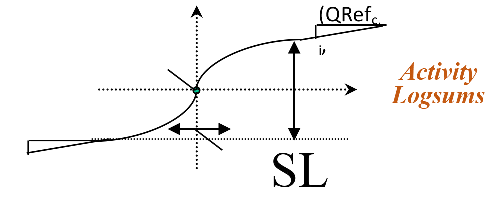
\includegraphics[scale=0.8]{aa/errant_figure_6_5}
\caption{Import function parameters}\label{fig:aa-import-parameters}
\end{figure}

The slope terms were set at 10 percent of the reference quantities (negative export slope) and the exponent at 20 percent, except for floorspace, as shown in Table \ref{tab:aa-ie-function-parameters}.

\begin{table}   % Table 6-11 AA Import/Export Function Parameters
\centering
\caption{AA import-export function parameters}\label{tab:aa-ie-function-parameters}
\begin{tabular}{lccccc|ccccc}
\hline
Commodity & \multicolumn{5}{c|}{Import coefficients} & \multicolumn{5}{c}{Export coefficients} \\
\cline{2-11}
categories & $QRef_{c,i}$ & ~$\gamma_{c,i}$~ & ~$\eta_{c,i}$~ & ~$\mu_{c,i}$~ & $PriceRef_{c,i}$ & $QRef_{c,e}$ & $~\gamma_{c,e}$~ & ~$\eta_{c,e}$~ & ~$\mu_{c,e}$~ & $PriceRef_{c,e}$ \\
\hline
All & 1e6 & 0.2 & 1e6 & 1e6 & 1 & 1e6 & 0.2 & -1e6 & -1e6 & 1 \\
\hline
\multicolumn{11}{l}{\footnotesize Note: $PriceRef$ values are S1 parameters (see \S\ref{sec:ned-s1-s2}) from AA input file ExchangeImportExportsI.csv}
\end{tabular}
\end{table}

\subsubsection{Import and export function parameters}
The bulk of import and exports are represented explicitly in the six world markets. Thus goods and services must travel along the highway network to reach the import/export exchange location, representing the costs of transporting these physical goods to the external markets. For more discussion of these world markets and associated assumptions see Sections \ref{sec:model-area-geography} (page \pageref{sec:model-area-geography}) and \ref{sec:category-definitions} (page \pageref{sec:category-definitions}).

These imports are ``made'' by the importing activities, while the exports are ``used'' by the exporting activities.  The quantity of these activities is developed in the aggregate economic flows table, and by the NED module for future years as part of the overall balancing of the economy. In the base year the activity constraint procedure is used to establish the constants ($Constant_{a,z}$, equation \ref{eq:6.02}) that are required to draw the imports and exports from and to the correct direction into and out of the model region. These constants are applied in future years so that the directionality tends to be maintained but can respond to transportation conditions.  

There is overall elasticity in these imports and exports, this elasticity was adjusted through the 
calibration of the $\lambda_{m,a}$ parameter for the importing and exporting activities.  

\subsubsection{Floorspace import parameters}

Each floorspace type has a supply function in a specific land use zone. The shape of the supply function is specified with parameters that are documented in this section, and the size (magnitude) of the supply function is scaled based on the inventory of the space in that zone.

FloorspaceSupplyI.csv file is described immediately below:
\begin{itemize}
\item $ZoneNumber$ is an integer value of land use zone (LUZ) that is the exchange location zone; a value of -1 indicates all land use zones not considered explicitly in other rows using single zone numbers in single rows for the commodity
\item $Commodity$ are text characters of name of commodity; this must match exactly the commodity name used in CommoditiesI;
\item $SupplyFunctionMidpointFactor$ is the real value of import function quantity of commodity imported to exchange location when the unit exchange price for commodity in exchange zone is at its import reference level $PriceIRef_c$; this is $QiRefc$ in equation 21 in the Theoretical Formulation document;
\item $SupplyFunctionMidpointPrice$ is the real value of import function reference price per unit for import of commodity; this is $PriceIRefc$ in equations 21 and 23 in the Theoretical Formulation document;
\item $SupplyFunctionEta$ is the real value of import function coefficient for sensitivity to difference in exchange price for commodity concerning increase in imports of commodity for exponent term; this is $\eta_{ic}$ in equation 23 in the Theoretical Formulation document;
\item $SupplyFunctionDeltaFactor$ is a real value of import function coefficient for the rate of increase in imports of commodity for exponent term; this is $\Delta_{ic}$ in equation 21 in the Theoretical Formulation document;
\item $SupplyFunctionSlopeFactor$ is the real value of import function coefficient for the rate of increase in imports of commodity for linear term; this is $\mu_{ic}$ in equation 21 in the Theoretical Formulation document;
\item $NoQuantityPrice$ is a real value of export reference price per unit for export of commodity; this is $PriceERefc$ in equations 22 and 24 in the Theoretical Formulation document;
\item $NoQuantitySlope$ is a real value of export function coefficient for the rate of increase in exports of commodity for linear term; this is $\mu_{ec}$ in equation 22 in the Theoretical Formulation document;
\item $MonitorExchange$ are text characters indicating whether interim values for the commodity in the exchange zone are to be written to the log file in order to monitor the AA Module solution algorithm; ``true'' indicates the interim values are to be written, ``false'' indicates the interim values are not to be written
\end{itemize}
\noindent For Oregon model ZoneNumber for each floorspace type is set to -1 and MonitorExchange is set to ``false'' for all of the floorspace types. The calibrated values are shown in Table \ref{aa-floorspace-import-parameters}.

\begin{sidewaystable}   % Table 6-12 AA Floorspace Import Parameters
\centering
\caption{AA floorspace import parameters}\label{aa-floorspace-import-parameters}
%\small
\begin{tabular}{lC{0.6in}C{0.6in}C{0.6in}C{0.6in}C{0.6in}C{0.6in}C{0.6in}}
\hline
Commodity & Supply function midpoint factor & Supply function midpoint price & Supply
function eta & Supply function delta factor & Supply function slope factor & No quantity price & No quantity slope \\
\hline
FLR Accommodation & 0.28 & 5 & 0.44 & 0.67 & 0.0008 & 5 & -1.3E-05 \\
\gray FLR Agriculture & 0.28 & 0.03 & 60 & 0.67 & 0.533 & 0.023 & -0.0222 \\
FLR Government Support & 0.28 & 5 & 0.55 & 0.67 & 0.00123 & 6.5 & -1.3E-05 \\
\gray FLR K12 & 0.28 & 5 & 0.55 & 0.67 & 0.0008 & 7 & -1.3E-05 \\
FLR Heavy Industry & 0.28 & 3.5 & 0.629 & 0.67 & 0.00114 & 7 & -1.3E-05 \\
\gray FLR Hospital & 0.28 & 5 & 0.55 & 0.67 & 0.0008 & 10 & -1.3E-05 \\
FLR Institutional & 0.28 & 5 & 0.55 & 0.67 & 0.0008 & 10 & -1.3E-05 \\
\gray FLR Light Industry & 0.28 & 3.5 & 0.629 & 0.67 & 0.00114 & 7 & -1.3E-05 \\
FLR Logging & 0.28 & 0.03 & 60 & 0.67 & 0.533 & 0.025 & -0.0889 \\
\gray FLR Office & 0.28 & 5 & 0.55 & 0.67 & 0.00123 & 7 & -1.3E-05 \\
FLR Retail & 0.28 & 5 & 0.44 & 0.67 & 0.000667 & 10 & -1.3E-05 \\
\gray FLR Warehouse & 0.28 & 3.5 & 0.629 & 0.67 & 0.00178 & 4.5 & -1.3E-05 \\
FLR MH & 0.056 & 0.15 & 1.1 & 0.804 & 0.01 & 6 & -3.3E-05 \\
\gray FLR MF & 0.056 & 0.15 & 1.1 & 0.804 & 0.01 & 6 & -3.3E-05 \\
FLR AT & 0.056 & 0.15 & 1.1 & 0.804 & 0.01 & 6 & -3.3E-05 \\
\gray FLR SFD & 0.056 & 0.15 & 1.1 & 0.804 & 0.01 & 6 & -3.3E-05 \\
FLR RRMH & 0.056 & 0.15 & 1.1 & 0.804 & 0.01 & 6 & -3.3E-05 \\
\gray FLR RRSFD & 0.056 & 0.15 & 1.1 & 0.804 & 0.01 & 6 & -3.3E-05 \\
\hline
\end{tabular}
\end{sidewaystable}

\section{Inputs and Outputs}\label{sec:aa-inputs-outputs}
The inputs and output of the AA module are listed in Tables \ref{tab:aa-inputs} and \ref{tab:aa-outputs}, respectively. The remainder of this section discusses them in more detail, including selected AA inputs and processing to generate base year input data.

\begin{sidewaystable}
\centering
\caption{AA module inputs}\label{tab:aa-inputs}
\begin{tabular}{L{4.5in}L{2.75in}L{1.1in}}
\hline
Data element & File(s) & Source \\
\hline

Modelwide total production quantity of activity $a$ ($TW_a$), modified by AA p-processor & ActivityTotalsI.csv, ActivityTotalsW.csv & NED (industry \$), SPG1 (HHs) \\

\gray Total production quantity of activity by alpha zone in the 2009 base year ($TW_{a,z}$), used to set zonal constants in constrainted AA run & ActivityConstraintsI.csv & Exogenous \\

Quantities of total floorspace inventory by alpha zone & FloorspaceI.csv & ALD \\

\gray Increments of total floorspace change in past year by alpha zone & Increments.csv & ALD \\

Fixed constant-production rate agricultural and forest lands by zone & AgForestFloorspace.csv (used only in AA, adds FloorspaceI.csv resource land sqft) & Exogenous \\

\gray Mode choice composite utility for commodity $c$ between beta zones $k$ and $z$ ($MSLogSum_{c,k,z}$) & **mcls\_beta.zmx & PT \\

Auto and commercial vehicle times and distances traveled by commodity $c$ between beta zones $k$ and $z$ ($Time_{c,k,z}$, $Dist_{c,k,z}$) & betapk***dist.zip, betapk***time.zip, worldZoneDistances.csv & VISUM \\

\gray Proportion of modelwide quantity of production activity $a$ in zone $z$ in the prior year ($PrevW_{a,z}$) & ActivityLocations.csv & Prev year AA \\

Unit prices for commodities by beta zones ($Price_{c,k}$) & ExchangeResults.csv (prior), ExchangeResultsI.csv (current) & Prev year AA \\

\gray Production size terms by zone $z$ and activity $a$ ($Size_{a,z}$) & ActivitySizeTermsI.csv & Exogenous \\

Aggregate activities definitions/parameters & ActivitiesI.csv & Exogenous \\

\gray Commodity definitions/parameters and transportation-based cost coefficients & CommoditiesI.csv & Exogenous \\

Floorspace constants & FloorspaceSupplyI.csv & Exogenous \\

\gray Industry technology options and related commodity make and use coefficients & TechnologyOptionsI.csv & Exogenous \\

Import/export function coefficients by beta zone & ExchangeImportExportI.csv & Exogenous \\

\gray List of alpha zones and beta zones & alpha2beta.csv, processed into FloorspaceZonesI.csv and PECASZonesI.csv & Exogenous \\

Index numbers used to identify activities and commodities in ZonalMakeUse.csv (only if stringsInZonalMakeUse is set to false in properties file) & ActivityNumbers.csv, CommodityNumbers.csv & Exogenous \\

\gray Trip length/time distribution input (optional) & HistogramsI.csv & Exogenous \\
\hline
\end{tabular}
\end{sidewaystable}   % Table 6-13 AA Inputs
\begin{sidewaystable}
\centering
\caption{AA module outputs}\label{tab:aa-outputs}
\begin{tabular}{L{4.25in}L{2.5in}L{1.5in}}
\hline
Data element & File(s) & User(s) \\
\hline
AA Working files (see above) & & AA \\
\gray Internal commodity dollar flows (goods, services, labor) between beta zones & buying\_commodity.zipMatrix, selling\_commodity.zipMatrix & PT (selling labor), CT (goods) \\

Labor dollar production by occupation and household category and consumption by occupation and industry expanded to alpha zones & TAZDetailedMake.csv, TAZDetailedUse.csv & SPG2 (production) \\

\gray Labor dollar production and consumption by occupation category expanded to alpha zones & laborDollarProductionSum.csv, laborDollarConsumptionSum.csv, FloorspaceZoneTotalMakeUse.csv & PT \\

Activity quantities and composite utilities for beta and alpha zones & ActivityLocations.csv, ActivityLocations2.csv & SPG2 (alpha), Next yr AA (beta) \\

\gray Occupied quantities and unit prices for floorspace in beta zones & ExchangeResults.csv & Next yr ALD \\

Import/export quantities of commodities (\$ flows) to beta zones & ExchangeResults.csv & CT diagnostics \\

\gray Commodity quantities make and use by alpha zone & FloorspaceZoneTotalMakeUse.csv, FloorspaceZoneTotalMakeUse.bin & CT (future) \\

Modelwide composite utilities of production by activity & ActivitySummary.csv & Next yr NED (future) \\

\gray Solved beta zone industry-commodity production and consumption technical coefficients & ZonalMakeUse.csv & Diagnostics \\

Commodity beta zone composite utilities & CommodityZUtilities.csv & Diagnostics \\

\gray Trip length distribution histogram output & Histograms.csv & Diagnostics \\

Summary totals from ZonalMakeUse.csv & MakeUse.csv & CT, diagnostics \\

\gray Summary totals from ExchangeResults.csv & ExchangeResultsTotals.csv & Diagnostics \\

Outcome of technology choice by each activity in each beta zone & TechnologyChoice.csv & Diagnostics \\

\gray Amount of flow that is intrazonal & PctIntrazonalxCommodityxBzone.csv & Diagnostics, calibration of short trips \\

Relative importance of commodity random utility error term for each activity, for buying & ProductionErrorTermSizes.csv & Diagnostics, advanced calibration \\

\gray Relative importance of commodity random utility error term for each activity, for selling & ProductionErrorTermSizes.csv & Diagnostics, advanced calibration \\
\hline
\end{tabular}
\end{sidewaystable}   % Table 6-14 AA Outputs 

AA produces the following working files pulling data from other modules, as listed above and 
discussed with the AA p-processor in \S\ref{sec:aa-p-processor}:
\begin{itemize}
\item {[ActivityTotalsW.csv] from [ActivityTotalsI.csv], [activity\_forecast.csv], [householdsByHHCategory.csv], [trade\_forecast.csv], [government\_forecast] and [TechnologyOptionsI.csv]}
\item {[FloorspaceW.csv] from [AgForestFloorspace.csv] and [FloorspaceI.csv]}
\item {[ActivitiesZonalValuesW.csv] from [ActivitiesZonalValuesI.csv], [Increments.csv] and [ActivityLocations.csv]}
\item {[TechnologyOptionsW.csv] from [TechnologyOptionsI.csv]}
\end{itemize}

\noindent A few notes on AA files:
\begin{itemize}
\item When AA looks for previous year prices, it first looks for ExchangeResultsI.csv in the current year 
directory and if not found, ExchangeResults.csv output from the previous year is used.
\item AA has an option to produce trip length/time histograms on request. To do so, the HistogramsI.csv input file must be specified with the following column fields: commodity name, skim (distance/time matrix), the upper bound of up to 100 trip length or time bands (typically miles/minutes). All commodities must have the same number of bands in the file, with zeros listed for any bands not used. Each listed commodity generates an output Histograms.csvfile with buying/selling quantity (commodity dollar value) that falls within each band, as well as the average trip length/time value of each band. One more band than the number of upper bounds, as the last band is values exceeding the upper-most band.
\end{itemize}

\subsection{Modelwide Activity by Category}
Each period, AA allocates modelwide production activity, $TW_a$ output from the NED module, among beta zones. The previous period's allocation by zone, $PrevWa,z$, influences the outcome of the current year. The number of households by income and household size categories is used as the measure of residential activity and as a size term, in the allocation of labor ($Sizea,z$) and the location of construction activity. Industry and government as well as import/export activity come from the NED module (activity\_forecast.csv, government\_forecast.csv, trade\_forecast.csv), while household counts come from the SPG1 module (householdsByHHCategory.csv). The AA pre-processor augments the NED industry output by adding office-based activity by industry.

Base year modelwide industry production (margined make) by activity in 2009 dollars used for $TW_a$ comes from 2009 IMPLAN data (with some adjustments to add office activity and adjust education activity dollars), also processed as part of the Make and Use Technical coefficients as discussed in \S\ref{sec:pa-allocation-parameters}. Base year modelwide household counts used as activity totals in AA are obtained from SPG1 module output. In the base year, SPG1 is constrained by the NED 2009 employment forecasts that are consistent with the 2009 IMPLAN industry activity data. 

Each year AA adds to these NED and SPG values by calculating the following (resulting in AA input file, ActivityTotalsI.csv):
\begin{itemize}
\item Modelwide amount of potential imports and exports based on the total internal use and total internal make in the previous year.  
\item Modelwide amount of office support activities based on the use of office support by the production activities.
\end{itemize}
\noindent The base year modelwide values are shown in Tables \ref{tab:aa-industry-production} through \ref{tab:aa-imports-exports}.

%Table 6-15 2009 Modelwideproduction by each activity in 2009 dollars
\begin{sidewaystable}
\centering
\caption{Modelwide industry production by activity, in 2009 dollars}
\label{tab:aa-industry-production}
\small
\begin{tabular}{lrr|lrr}
\hline
Activity - Industry & Total amount in 2009 & 2009 employees & Activity - Industry & Total amount in 2009 & 2009 employees \\
\hline
RES\_agmin\_ag & 16,903,898,303 & 102,010 & TRNS\_trns\_off & 2,125,367,253 & 45,390 \\
\gray RES\_forst\_log & 2,519,144,897 & 8,212 & INFO\_info\_off\_li & 15,239,006,202 & 6,691 \\
RES\_offc\_off & 1,332,074,223 & 58,746 & INFO\_info\_off & 2,881,870,409 & 49,465 \\
\gray ENGY\_elec\_hi & 8,621,276,855 & 6,642 & UTL\_othr\_off\_li & 8,378,148,941 & 18,973 \\
ENGY\_ngas\_hi & 3,603,145,996 & 696 & UTL\_othr\_off & 1,114,027,683 & 11,593 \\
\gray ENGY\_ptrl\_hi & 4,631,318,359 & 1,760 & FIRE\_fnin\_off & 31,902,799,194 & 150,467 \\
ENGY\_offc\_off & 1,912,330,649 & 9,839 & FIRE\_real\_off & 15,446,998,046 & 139,527 \\
\gray CNST\_main\_xxx & 3,690,346,435 & 22,722 & HLTH\_hosp\_hosp & 12,295,007,812 & 88,868 \\
CNST\_nres\_xxx & 6,542,617,309 & 60,252 & HLTH\_care\_inst & 3,849,533,203 & 68,309 \\
\gray CNST\_othr\_xxx & 8,729,001,953 & 32,922 & HLTH\_othr\_off\_li & 18,144,155,090 & 130,909 \\
CNST\_res\_xxx & 6,740,919,189 & 44,474 & K12\_k12\_k12 & 12,626,084,053 & 171,266 \\
\gray CNST\_offc\_off & 2,666,187,151 & 53,353 & K12\_k12\_off & 2,777,603,399 & 55,024 \\
MFG\_food\_hi & 10,829,728,776 & 23,936 & HIED\_hied\_off\_inst & 4,569,757,377 & 79,243 \\
\gray MFG\_food\_li & 10,829,728,776 & 15,123 & ENT\_ent\_ret & 3,571,715,370 & 79,205 \\
MFG\_htec\_hi & 13,063,887,807 & 9,623 & HOSP\_acc\_acc & 3,539,955,230 & 35,959 \\
\gray MFG\_htec\_li & 13,063,887,807 & 5,323 & HOSP\_eat\_ret\_acc & 12,374,280,273 & 219,249 \\
MFG\_hvtw\_hi & 14,441,531,006 & 40,903 & SERV\_tech\_off & 22,817,588,607 & 219,409 \\
\gray MFG\_hvtw\_li & 14,441,531,006 & 35,469 & SERV\_site\_li & 5,828,886,779 & 57,739 \\
MFG\_lvtw\_hi & 12,978,764,067 & 18,393 & SERV\_home\_xxx & 456,867,797 & 54,769 \\
\gray MFG\_wdppr\_hi & 11,847,955,596 & 34,188 & SERV\_bus\_off & 14,387,504,547 & 172,891 \\
MFG\_offc\_off & 10,165,454,716 & 115,552 & SERV\_nonp\_off\_inst & 9,376,816,406 & 133,060 \\
\gray WHSL\_whsl\_ware & 19,829,592,529 & 111,388 & SERV\_stor\_ret & 5,164,732,788 & 80,744 \\
WHSL\_offc\_off & 1,733,860,878 & 23,800 & GOV\_admn\_gov & 19,036,836,853 & 80,323 \\
\gray RET\_auto\_ret & 7,439,574,272 & 99,409 & GOV\_offc\_off & 10,008,657,941 & 184,378 \\
RET\_stor\_ret & 16,026,845,092 & 254,174 & FGOV\_acct\_gov & 93,817,953,918 & 0 \\
\gray RET\_stor\_off & 1,518,361,266 & 31,948 & SLGOV\_acct\_gov & 71,879,103,322 & 0 \\
RET\_nstor\_off & 2,193,797,363 & 44,300 & CAP\_acct\_gov & 69,549,704,567 & 0 \\
\gray TRNS\_trns\_ware & 14,723,200,435 & 66,561 &  &  &  \\
\hline
\end{tabular}
\end{sidewaystable}


\begin{table}   % Formerly Table 6-16
\centering
\caption{Modelwide household production by activity, in 2009 dollars}\label{tab:production-activity}
\begin{tabular}{lr|lr}
\hline
Activity--Households & Total 2011 amount & Activity--Households & Total 2011 amount \\
\hline
HH0to8k1to2 & 114,469 & HH32to46k3plus & 126,609 \\
\gray HH0to8k3plus & 23,154 & HH46to61k1to2 & 196,680 \\
HH8to15k1to2 & 166,181 & HH46to61k3plus & 136,043 \\
\gray HH8to15k3plus & 37,181 & HH61to76k1to2 & 133,215 \\
HH15to23k1to2 & 179,197 & HH61to76k3plus & 120,596 \\
\gray HH15to23k3plus & 59,952 & HH76to106k1to2 & 154,108 \\
HH23to32k1to2 & 187,491 & HH76to106k3plus & 170,804 \\
\gray HH23to32k3plus & 80,364 & HH106kUp1to2 & 153,655 \\
HH32to46k1to2 & 240,622 & HH106kUp3plus & 176,127 \\
\hline
\end{tabular}
\end{table}

%Table 6-17 Modelwide import and exports for each commodity in 2009 dollars
\begin{sidewaystable}
\centering
\caption{Modelwide imports and exports for each commodity, in 2009 dollars}
\label{tab:aa-imports-exports}
\small
\begin{tabular}{lrr|lrr}
\hline
Activity & Imports & Exports & Activity & Imports & Exports \\
\hline
sctg01\_fkp\_lvsk & 260,851,452 & 402,771,058 & sctg30\_oth\_clth & 3,501,242,543 & 517,835,114 \\
\gray sctg02\_fkp\_agri\_cereal & 591,333,272 & 485,384,922 & sctg31\_cms\_min & 1,356,212,151 & 877,088,616 \\
sctg03\_fkp\_agri\_other & 1,099,383,757 & 6,652,824,240 & sctg32\_mit\_metl\_base & 3,520,421,862 & 3,018,300,425 \\
\gray sctg04\_fkp\_feed & 763,912,960 & 157,695,428 & sctg33\_mit\_metl\_prod & 2,704,359,252 & 2,533,120,109 \\
sctg05\_fkp\_food\_meat & 2,921,116,467 & 2,043,552,639 & sctg34\_mit\_mach & 7,315,651,539 & 4,377,044,071 \\
\gray sctg06\_fkp\_agri\_grain & 855,005,202 & 761,763,359 & sctg35\_mit\_elct & 11,314,880,451 & 21,885,691,855 \\
sctg07\_fkp\_food\_prep & 5,311,390,317 & 9,382,925,853 & sctg36\_mit\_tran & 6,976,890,863 & 3,168,379,696 \\
\gray sctg08\_fkp\_food\_alc & 1,431,454,151 & 1,156,635,454 & sctg37\_mit\_inst\_transp & 2,147,223,976 & 2,603,475,287 \\
sctg10\_cms\_clay & 73,318,169 & 95,534,556 & sctg38\_mit\_inst\_prec & 3,143,044,038 & 2,301,165,169 \\
\gray sctg11\_cms\_sand & 17,333,501 & 163,311,587 & sctg39\_oth\_furn & 1,872,685,394 & 1,103,630,305 \\
sctg13\_cms\_mine\_nonmet~~~~~~~~~~ & 144,903,688 & 34,035,256 & sctg40\_oth\_misc & 4,774,667,512 & 1,856,532,608 \\
\gray sctg14\_cms\_mine\_met & 507,173,011 & 1,315,595,424 & sctg41\_waste\_scrap & 470,266,803 & 514,256,780 \\
sctg15\_pcc\_coal & 717,887,113 & 34,023,971 & higher\_education & 832,993,534 &  \\
\gray sctg16\_pcc\_petr\_crude & 1,590,154,115 & 242,077,538 & energy & 1,143,833,082 & 3,123,152,392 \\
sctg17\_pcc\_fuel & 5,642,668,465 & 21,714,405 & retail\_trade & 1,961,754,163 & 3,929,056,354 \\
\gray sctg18\_pcc\_petr\_oil & 2,821,334,232 & 10,857,202 & transport & 3,101,392,984 & 3,152,134,411 \\
sctg19\_pcc\_coal\_prod & 4,069,050,714 & 200,319,354 & wholesale\_trade & 2,033,744,399 & 3,135,668,823 \\
\gray sctg20\_pcc\_chem\_basic & 1,891,511,255 & 1,126,536,613 & construction & 12,590,735,942 & 9,180,101,387 \\
sctg21\_pcc\_chem\_pharma & 6,235,158,377 & 764,919,598 & communications\_and\_utilities & 7,869,734,616 & 5,678,834,996 \\
\gray sctg22\_pcc\_chem\_fert & 404,925,018 & 179,061,241 & accommodations & 2,541,892,752 & 3,270,897,187 \\
sctg23\_pcc\_chem\_prod & 3,300,069,335 & 994,754,044 & personal\_and\_other\_services\_and\_amusements & 1,871,340,674 & 4,882,028,098 \\
\gray sctg24\_pcc\_petr\_plast & 4,398,887,943 & 2,051,431,134 & entertainment\_services & 1,089,285,393 & 407,917,914 \\
sctg25\_fwp\_logs & 340,809,605 & 1,101,015,179 & food\_services & 333,886,154 & 720,016,802 \\
\gray sctg26\_fwp\_wood & 651,283,882 & 4,716,264,380 & health\_services & 1,230,526,561 & 928,962,118 \\
sctg27\_ppp\_papr\_puplp & 840,672,962 & 4,508,321,602 & fire\_business\_and\_professional\_services & 30,845,752,639 & 6,322,315,673 \\
\gray sctg28\_ppp\_papr\_paper & 1,240,237,671 & 757,806,729 & government\_administration & 3,567,099,663 & 8,268,890,580 \\
sctg29\_ppp\_papr\_print & 1,703,591,533 & 913,103,214 & education\_reports\_to\_sponsors & 37,468,124 & 3,594,244,993 \\
\hline
\end{tabular}
\end{sidewaystable}

\subsection{Floorspace Quantities by Category by Zone}\label{sec:aa-floorspace-quantities}
Floorspace is an important AA input. It establishes the available exchange locations for production activities. It is received as a fixed amount of space, from the ALD module. For the base year, floorspace quantities by industry and zone (alpha zone, aggregated to beta zones for use in AA) were generated synthetically for ALD. The development of the base year floorspace estimate is discussed in \S\ref{sec:ald-baseyear-floorspace} (page \pageref{sec:ald-baseyear-floorspace}).

In AA agriculture and logging resource lands are treated slightly differently than in ALD. AA requires a consistent use of floorspace per employee per year in a given industry. Resource lands are also less available in urban areas. A base year estimate of the resource lands was developed based on zoning coverage and used as a constraint on allocation of base year employees using these resource lands (see \S\ref{sec:ald-baseyear-floorspace} and \S\ref{sec:aa-zonal-activity-targets}). Selected locations in the halo counties and outside of Oregon UGBs were allowed to exceed the zoning restriction. In both, agriculture and forestry production activities, a single acre per employee usage rate was assumed for each industry employee. This is a simplification of prior PI-based assumptions of 9.1 and 50.1 acres/employee for ag/mining and forestry/logging, respectively (representing the most intensive acres per agriculture employee of the modeled counties).  

The result is a base year amount of land available to AA (AgForFloorspace.csv). These lands (quantity and location) are assumed to be fixed for the duration of the model. In the future, a more sophisticated submodel could be built to address the different land use intensities of agriculture and timberlands, urban-rural conversion of lands, as well as annually rotate timber harvests to un-cut timberland.

\subsection{Road Network Travel Conditions}
AA location decisions are influenced by transport costs and times to obtain factor inputs and reach markets. In addition the composite utility of personal travel across all modes is used in AA, calculated for the previous year in the PT module. 

AM peak period (7-9 AM) auto travel times and costs (both outbound and return) are used for goods and selected service commodities. Identification of the imports/exports of goods commodities requires the multimodal networks used for network assignment to include travel conditions to/from the world market zones (6000 zones). Commercial vehicle skims will be used for selected goods commodities when they become available, allowing industry response to weight restrictions (i.e., increased heavy truck transport costs influence industry location decisions). PT-generated peak mode choice composite utility values,based on time and cost across all modes of travel, are used to represent the travel conditions for labor flows and selected personal services. The assumed travel skims are listed in Table \ref{tab:assumed-network-conditions} for all commodities (AA input CommoditiesI.csv).

These PT outputs are in a compressed OD matrix format, ``squeezed'' from alpha to beta zones for use in the AA module. Initial values were provided by loading the model networks used in the highway and transit network assignment modules. The base year employs preliminary output developed from metro area data. 

% Table 6-18 Assumed Network Travel Conditions by Commodity
\begin{table}
\centering
\caption{Assumed network travel conditions by commodity}
\label{tab:assumed-network-conditions}
\small
\begin{tabular}{ll}
\hline
Commodity & Travel skim(s) \\
\hline
\rowcolor{orange!20}\multicolumn{2}{l}{\textit{Goods commodities}} \\
All SCTG goods commodities & betapktrk1time, betapktrk1dist, betapktrk1toll \\
\rowcolor{orange!20}\multicolumn{2}{l}{\textit{Occupation Labor Commodities}} \\
A1-Mgmt Bus & w7mcls\_beta \\
\gray B1-Prof Specialty & w7mcls\_beta \\
B2-Education & w4mcls\_beta \\
\gray B3-Health & w7mcls\_beta \\
B4-Technical Unskilled & w1mcls\_beta \\
\gray C1-Sales Clerical Professionals & w4mcls\_beta \\
C2-Sales Service & w4mcls\_beta \\
\gray C3-Clerical & w4mcls\_beta \\
C4-Sales Clerical Unskilled & w1mcls\_beta \\
\gray D1-Production Specialists & w4mcls\_beta \\
D2-MaintConstRepair Specialists & w4mcls\_beta \\
\gray D3-ProtectTrans Specialists & w4mcls\_beta \\
D4-Blue Collar Unskilled & w1mcls\_beta \\
\gray A1-Mgmt Bus & w7mcls\_beta \\
\rowcolor{orange!20}\multicolumn{2}{l}{\textit{Service Commodities}} \\
Retail Trade & s4mcls\_beta \\
\gray Transport & betapkautotime, betapkautodist, beetapkautotoll \\
Wholesale Trade & betapkautotime, betapkautodist, beetapkautotoll \\
\gray Construction & betapkautotime, betapkautodist, beetapkautotoll \\
Communications and Utilities & betapkautotime, betapkautodist, beetapkautotoll \\
\gray Accommodations & betapkautotime, betapkautodist, beetapkautotoll \\
Personal and Other Services and Amusements & b5mcls\_beta \\
\gray Entertainment Services & b5mcls\_beta \\
Food Services & b5mcls\_beta \\
\gray Teaching K12 & c4mcls\_beta \\
Higher Education & c4mcls\_beta \\
\gray Health Services & o4mcls\_beta \\
Fire Business and Professional Services & betapkautotime, betapkautodist, beetapkautotoll \\
\gray Government Administration & b4mcls\_beta \\
Internal Services (all types) & b8mcls\_beta \\
\hline
{\footnotesize where:} \\
\multicolumn{2}{l}{\footnotesize Peak period (7-9AM) auto network distance between beta zones [betapkdist.zip]} \\
\multicolumn{2}{l}{\footnotesize Peak period (7-9AM) auto network travel time between beta zones [betapktime.zip]} \\
\multicolumn{2}{l}{\footnotesize Peak period (7-9AM) auto network travel time between beta zones [betapktime.zip]} \\
\multicolumn{2}{l}{\footnotesize Mode choice logsum for Work trips, $<$\$15K income, number of autos=0 [w1betals.zip]} \\
\multicolumn{2}{l}{\footnotesize Mode choice logsum for Work trips, \$15-30K income, number of autos $<$ household size [w4betals.zip]} \\
\multicolumn{2}{l}{\footnotesize Mode choice logsum for Work trips, $>$\$30K income, number of autos<household size [w7betals.zip]} \\
\multicolumn{2}{l}{\footnotesize Mode choice logsum for Work-based trips, \$15-30K income, number of autos $<$ household size [b4betals.zip]} \\
\multicolumn{2}{l}{\footnotesize Mode choice logsum for Work-based trips, \$15-30K income, number of autos $\ge$ household size [b5betals.zip]} \\
\multicolumn{2}{l}{\footnotesize Mode choice logsum for Work-based trips, $>$\$30K income, number of autos $\ge$ household size [b8betals.zip]} \\
\multicolumn{2}{l}{\footnotesize Mode choice logsum for School trips, \$15-30K income, number of autos $<$ household size [c4betals.zip]} \\
\multicolumn{2}{l}{\footnotesize Mode choice logsum for Shopping trips, \$15-30K income, number of autos$<$household size [s4betals.zip]} \\
\multicolumn{2}{l}{\footnotesize Mode choice logsum for Other trips, \$15-30K income, number of autos$<$household size [o4betals.zip]} \\
\end{tabular}
\end{table}

\section{Calibration Targets}

AA has many avenues for calibration. The six formal PI calibration targets are listed in the top of Table \ref{tab:aa-calibration-targets}. These were used to formally assess AA calibration efforts. A tier-based approach to using these targets to calibrate AA over time, achieving the most important performance earlier in the project schedule, is discussed in \S\ref{sec:aa-initial-calibration} (page \pageref{sec:aa-initial-calibration}). The remainder of this section discusses the listed data sources in more detail.

%Table 6-19  AA Calibration Targets
\begin{table}[!t]
\centering
\caption{AA calibration targets}\label{tab:aa-calibration-targets}
\small
\begin{tabular}{p{1.95in}cp{3.4in}}
\hline
Source & Year(s) & SWIM2 Target \\
\hline
\rowcolor{orange!20}\multicolumn{3}{l}{\textit{Zonal Activity Targets (ActivityConstraintsI.csv)}} \\
Employment data & 2009 & Zonal Employment by industry/ \\
\gray IMPLAN County disaggregated with QCEW (Oregon) and OnTheMap Census (halo) & 2009, 2008 & occupation (converted to industry dollars)\\
American Community Survey (ACS) Household data & 2009 & Zonal Household by income and size \\
\gray FHWA Freight Analysis Framework (FAF3) & 2009 & Modelwide imports/exports (\$) by commodity and world market \\
\rowcolor{orange!20}\multicolumn{3}{l}{\textit{Trip Length Targets (histogramsI.csv)}} \\
FHWA FAF3 data & 2007 & Average trip length by goods commodity \\
\gray Oregon Travel Behavior Surveys & 1994-96 & Personal trip length distributions by purpose/occupation \\
Ohio Establishment Survey & 2003 & Average trip lengths by business services \\
\rowcolor{orange!20}\multicolumn{3}{l}{\textit{Price Targets (ExchangeResultsTargetsI.csv)}} \\
ACS PUMS & 2009 & HH use of dwelling type and size, HH make of labor occupation dollars, industry use of labor and floorspace \\
\gray Urban Real Estate Reports (Bend-Redmond, Eugene-Springfield, Medford, Portland-Vancouver) & 1998-99 & Average home sales and apartment rents and office, retail and industry floorspace rates by real estate area, vacancy Rates by floorspace type by real estate area \\
\rowcolor{orange!20}\multicolumn{3}{l}{\textit{Commodity and Labor Flow Targets}} \\
ACS PUMS & 2005-09 & POWPUMA-PUMA labor flows, wage dollars by occupation \\
\gray FHWA FAF3 data & 2007 & Goods flows (\$) in, out, and within Oregon \\ 
\rowcolor{orange!20}\multicolumn{3}{l}{\textit{Other Targets}} \\
Portland Metro 2009 Housing Needs Analysis Report & 2009-30 & Portland Metro Demographic Forecasts (see \S\ref{sec:metroscope-forecast}) \\
\hline
\end{tabular}
\end{table}

\subsection{Zonal Activity Targets}\label{sec:aa-zonal-activity-targets}
Alpha zone quantities of activity provide a target for AA allocations in a single year. The totals must match the totals in ActivityTotalsI.csv for that year.  When run in ``constrained'' mode, AA produces zonal constants required to meet these zonal constraints at the beta zone level. These zonal targets are specified in the file ActivityConstraintsI.csv and include: 
\begin{itemize}
\item Industry activity (in dollars), based on employment by zone
\item Household counts
\item Modelwide Imports and Exports of goods and services exchanged with each world market (labor 
is not exchanged)
\end{itemize}

\subsubsection{Employment by Industry}

2009 IMPLAN employment was obtained for the 75 counties in the study area and aggregated to match AA industries (all except office support sectors, see Table \ref{tab:activity-industry} on page \pageref{tab:activity-industry}). County employment estimates by industry were then allocated to aggregated alpha zones using 2009 Quarterly Census of Employed Workers (QCEW) data within Oregon (geocoded) and 2008 US Census OntheMap data (by place of work) in the halo (block group). The categories of these latter sources required some aggregation of industry sectors to map to AA, as shown in Table \ref{tab:aa-industry-aggregation-zonal}. 

\begin{sidewaystable}
\centering
\caption{Aggregation of AA industries for use with zonal data (QCEW and OnTheMap)}
\label{tab:aa-industry-aggregation-zonal}
\footnotesize
\begin{tabular}{L{1.7in} L{1.9in} L{3in} L{1.6in}}
\hline
AA industries & QCEW industries (Oregon) & QCEW NAICS codes & OnTheMap industries (halo) \\
\hline
ENT\_ent\_ret & Entertainment & 711110-713990 & Entertainment \\
\gray FIRE\_fnin\_off & Finance and Insurance & 521110-525990, 533110 & FinanceandInsurance \\
FIRE\_real\_off & Real Estate & 531110-531390 & Services \\
\gray GOV\_admn\_gov, GOV\_offc\_off & Government Administration & 921110-928120 & Government \\
HIED\_hied\_off\_inst & Education-Higher & 611210-611699 & EducationalServices \\
\gray K12\_k12\_k12, K12\_k12\_off & Education-K12 & 611110, 611710 & EducationalServices \\
 & Education-86K12+14HIED & 518210, 541214 & EducationalServices \\
\gray HOSP\_acc\_acc & Accommodations & 721110-721310 & AccommodationandFoodServices \\
HOSP\_eat\_ret\_acc & Eating and Drinking Places & 722110-722410 & AccommodationandFoodServices \\
\gray HLTH\_care\_inst & Health Care Facility & 623110-623990 & Services \\
HLTH\_hosp\_hosp & Health-Hospital & 622110-622310 & Services \\
\gray HLTH\_othr\_off\_li & Health-Other & 621111-621999 & Services \\
SERV\_bus\_off & Services-Business & 551112-561210, 561410-561622, 561910-561990 & Services \\
\gray SERV\_home\_xxx & Services-at Customer's House & 814110 & Services \\
SERV\_nonp\_off\_inst & Services-Nonprofit & 624110-624310, 813110-813990 & Services \\
\gray SERV\_site\_li & Services-at Customer's Business & 532411-532490, 561710-561790, 811211-811490 & Services \\
SERV\_stor\_ret & Services-Storefront & 532210-532310, 624410, 812111-812990 & Services \\
\gray SERV\_tech\_off & Services-Professional and Technical & 541110-541990 (except 541214), 561311-561330 & Services \\
RET\_auto\_ret & Retail-Automotive+services & 441110-441320, 447110, 447190, 454111-454390, 532111-532120, 811111-811198 & RetailTrade \\
\gray RET\_nstor\_off & Retail-Nonstore &  &  RetailTrade \\
RET\_stor\_ret, RET\_stor\_off & Retail-Store & 442110-453998 (except 447110, 447190) & RetailTrade \\
\gray WHSL\_whsl\_ware, WHSL\_offc\_off & Wholesale & 423110-425120 (except 424710, 493190), 493110-493130 & WholesaleTrade \\
ENGY\_ptrl\_hi$^a$ & Wholesale-80Whse+20Engy-petro & 424710, 493190 & WholesaleTrade \\
\gray CNST\_othr\_xxx$^a$ & Construction-Other & 237110-237130, 237310-237990 & Construction \\
CNST\_res\_xxx, CNST\_nres\_xxx, CNST\_main\_xxx$^a$ & Construction-Buildings & 236115-236220, 237210 & Construction \\
\gray RES\_agmin\_ag$^a$ & Resource-Ag and Mining & 111120-112990, 114111-213115 & Resource \\
\hline
\multicolumn{4}{r}{\emph{Continued on next page}}
\end{tabular}
\end{sidewaystable}

\begin{sidewaystable*}
\centering
\footnotesize
\begin{tabular}{L{1.7in} L{1.9in} L{3in} L{1.6in}}
\hline
AA industries & QCEW industries (Oregon) & QCEW NAICS codes & OnTheMap industries (halo) \\
\hline
RES\_forst\_log$^a$ & Resource-Forest & 113110-113310 & Resource \\
\gray MFG\_food\_hi, MFG\_food\_li$^a$ & Manufacturing-Food & 238992-312140 & Manufacturing \\
MFG\_htec\_hi, MFG\_htec\_li$^a$ & Manufacturing-High Tech & Manufacturing &  \\
\gray MFG\_hvtw\_hi, MFG\_hvtw\_li$^a$ & Manufacturing-High VTW & 313111-316999, 322211-323122, 325411-325414, 326111-326299, 332111-333999, 335110-339999 & Manufacturing \\
MFG\_lvtw\_hi$^a$ & Manufacturing-Low VTW & 324110-325320, 325510-325998, 327111-331528, 334111-334612 & Manufacturing \\
\gray MFG\_wdppr\_hi$^a$ & Manufacturing-Wood and Paper & 32113-322130 & Manufacturing \\
INFO\_info\_off\_li, INFO\_info\_off & Information & 511110-519130 (except 518210) & Information \\
\gray TRNS\_trns\_ware, TRNS\_trns\_off & Transport & 481111-492210 & TransportationandWarehousing \\
UTL\_othr\_off\_li, UTL\_othr\_off & Utilities-Other & 221310-221320, 562111-562998 & Utilities \\
\gray ENGY\_elec\_hi$^a$ & Energy-Electric & 221111-221122 & Utilities \\
ENGY\_ngas\_hi$^a$ & Energy-Natural Gas & 221210 & Utilities \\
\gray  & NA & 238111-238992, 519190,999999 &  \\
\hline
\end{tabular}
\end{sidewaystable*}  % Table 6-22

This aggregated industry alpha zone employment was used as control totals in the development of an employment synthesizer. The employment synthesizer uses constraints and iteratively develops a disaggregate employment set with associated industry and alpha zone attributes to meet them. A score is developed based on the weighted constraints, and is improved with each iteration until a user-specified threshold is met. The following constraints were used in the employment synthesizer: 
\begin{itemize}
\item \textit{Industry by Individual TAZ}: As described above, data from the Bureau of Labor Statistics' (BLS) Covered Employment and Wages Program (ES-202 program) for the state of Oregon and from the Census Bureau's OnTheMap dataset for the halo zones surrounding Oregon were used to produce industry-level employment totals by TAZ for each of the 34 industries. An additional target was added for total employment by TAZ, to add additional emphasis on getting the right amount of employment in each zone. 
\item \textit{PECAS occupation by POWPUMA}: There are 31 of Place of Work Public Use Microdata Areas (POWPUMAs) in the study area, with 13 in Oregon. PUMS data has work location coded at this level, which is an aggregation of PUMAs and thus a very general geography; the entire three-county metro Portland area is a single POWPUMA. The 13 occupation groups used in the PECAS model were used for categories here, with the targets being the proportion of workers in each occupation group.
\item \textit{SOC occupation by Place and Place-remainders}: 
The Census Transportation Planning Package (CTPP) provides totals for legal places, such as counties or cities above 20,000 population; from these, remainder values were calculated to represent the remaining areas, with a total of 101 places in the study area. While this dataset breaks out the significant urban areas from the surrounding countryside, it uses an aggregation of the Standard Occupation Classification (SOC) coding system that is not entirely consistent with the model occupation groups. The proportion of workers in the 24 occupation groups were used as targets.
\item \textit{Split ratios by intensity areas:} The TAZ were classified into a set of 8 intensity levels ranging from effectively rural to very 
dense central business districts. The formula used for intensity was based on previous work in 
Oregon and Portland Metro modeling. The land use intensity, LUI, for a given zone $z$ is:
\begin{equation}
LUI_z = ln [(2.5*Employment_z  + Population_z)/Total Acres_z]
\end{equation}
\noindent For each intensity level and industry to be split, a target represents the proportion of workers in that industry performing office support work. For instance, 50 percent of the retail workers in the highest density zones are support workers, versus only five percent in the least dense zone categories. To develop these targets, for each industry, a total number of support workers was taken from PUMS, and the number of workers by intensity level was taken from the TAZ level industry totals. The proportion of support workers by intensity level was then developed using professional judgment to match the aggregate number of support workers, while being consistent with the idea that support work is primarily done in denser, downtown areas.
\end{itemize} 

Each zone in the model area was categorized into the above four target sets. For instance, the zone representing downtown Corvallis will have employment by industry targets for the specific zone, but the jobs here will also be considered in the fit of employment by SOC occupation targets for the city of Corvallis, the employment by PECAS occupation targets for POWPUMA 600 (Benton and Linn counties), and have production/support split targets as part of the intensity level 8 zones, along with other downtown zones in Portland, Salem, etc.

These nesting geographies are shown in Figure \ref{fig:aa-synthesis-geographies}. The top image shows the 13 POWPUMAs in Oregon, with POWPUMA 600 in purple. The central image shows the four CTPP geographies for POWPUMA 600; Benton county on the left in teal and Linn on the right in lime green, with the cities of Corvallis and Albany in orange and dark red. The bottom image shows the intensity levels by TAZ for the Corvallis-Albany-Lebanon area, with blue representing the lowest intensity and red the highest.

\begin{figure}   % Formerly Figure 6-6
\centering
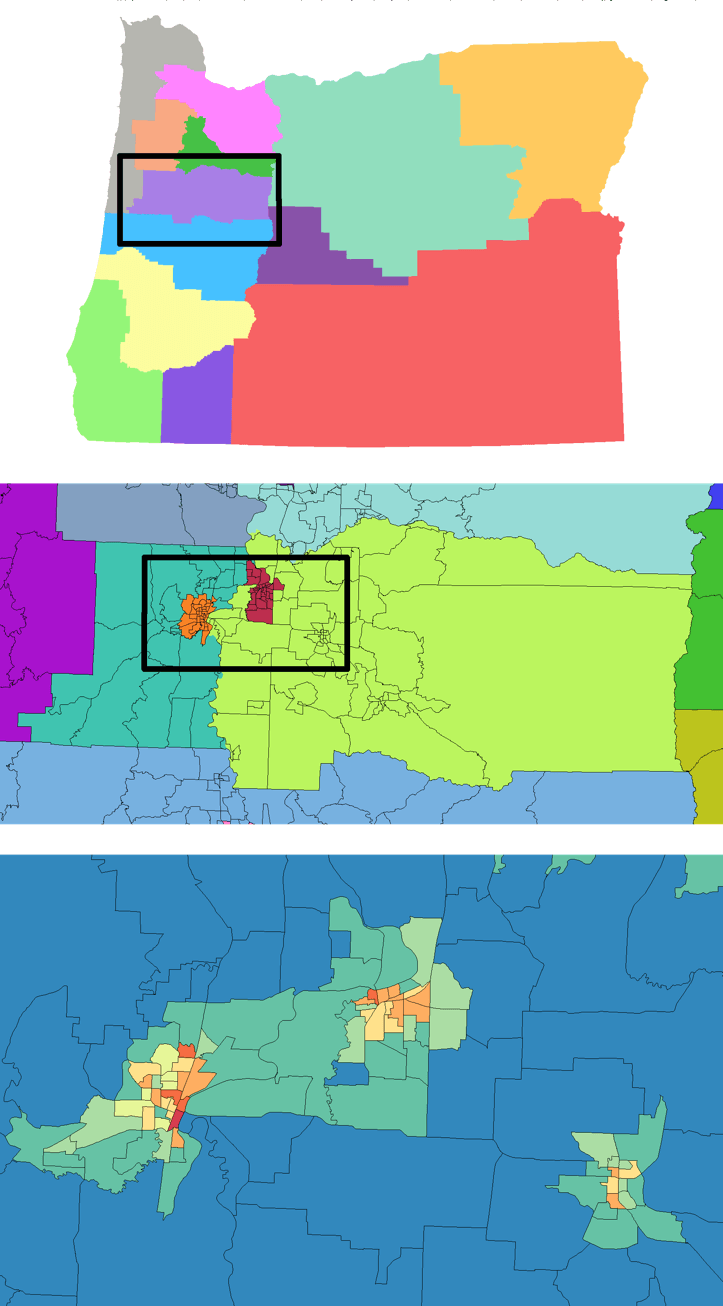
\includegraphics[scale=0.475]{aa/synthesis-geographies}
\caption{Synthesis geographies example}\label{fig:aa-synthesis-geographies}
\end{figure}

Each job in the PUMS file was also categorized based on these four categories; industries were coded by PECAS industry, occupations by both PECAS and CTTP codes, and a series of dummy variables indicated if a job was within one of the split industries, and if so, if it was one of the occupation groups considered to be a support function. (The definitions of support functions varied slightly by industry; the education occupation group is office support in most industries --- except in education industries, where it is the primary group of production workers.)

The employment by industry totals had a weight of 1; the other three target sets were proportions rather than absolute numbers of workers, so their targets were scaled appropriately. The weights developed were intended to emphasize matching the PECAS occupation groups ahead of the intensity groups or the CTPP groups. The relative weights were 2000, 500 and 250 respectively. 

The use of the industry split targets in the synthesizer means that industry management that occurs in office space was separated from line industry employment during the synthesis. Land use intensity (LUI) in any zone is calculated as a logged scale of combined population and employment per unit area. 
\begin{equation}\label{eq:6.41}
LUI_z = ln[(2.5*Employment_z  + Population_z)/Total Acres_z]
\end{equation}
\noindent This approach allows the share of management support workers to vary by industry-occupation combination and land use intensity. The assumed percent office support by industry and land use intensity used in the update are shown in Table \ref{tab:percent-office}. 

% Table 6-20 Assumed base year Percent Office Support by Industry and LU Intensity
\begin{table}
\centering
\caption{Assumed base year percent office support by industry and land use intensity}\label{tab:percent-office}
\begin{tabular}{lrrrrrrrr}
\hline
\multirow{2}{*}{Sector} & \multicolumn{8}{c}{Intensity range} \\
\cline{2-9}
& $<$-1 & -1 to 1 & 1 to 1.5 & 1.5 to 2 & 2 to 2.5 & 2.5 to 3.5 & 3.5 to 5 & $>$5 \\
\hline
Resources      & 10.0 & 59.2 & 68.5 & 74.7 & 79.6 & 83.5 & 87.0 &  90.0 \\
\gray Energy         & 25.0 & 25.3 & 27.2 & 31.9 & 40.5 & 54.0 & 73.6 & 100.0 \\
Construction   &  5.0 &  9.4 & 15.0 & 21.3 & 28.0 & 35.1 & 42.4 &  50.0 \\
\gray Manufacturing  &  5.0 & 10.6 & 19.7 & 31.0 & 43.8 & 58.1 & 73.5 &  90.0 \\
Wholesale      &  5.0 &  5.0 &  5.6 &  7.3 & 11.3 & 18.9 & 31.2 &  50.0 \\
\gray Retail         &  5.0 &  5.0 &  5.0 &  5.0 &  5.3 &  7.2 & 16.2 &  50.0 \\
Transportation & 10.0 & 12.9 & 19.5 & 28.9 & 40.9 & 55.2 & 71.6 &  90.0 \\
\gray Information    & 25.0 & 50.0 & 62.0 & 71.5 & 79.7 & 87.0 & 93.7 & 100.0 \\
Utilities      & 10.0 & 17.0 & 26.7 & 37.7 & 49.7 & 62.5 & 76.0 &  90.0 \\
\gray Education      &  5.0 &  6.0 &  8.9 & 13.6 & 20.1 & 28.3 & 38.3 &  50.0 \\
Government     & 25.0 & 25.3 & 27.2 & 32.0 & 40.7 & 54.2 & 73.7 & 100.0 \\
\hline
\end{tabular}
\end{table}

% Apparently A-F in this area, so need to reformat this to be in subsubsections

This production/support split could only be done for the zones in Oregon, as well as Clark County WA, where the zone system was fine enough to support this detailed level of land use intensity analysis. In the remainder of the halo, the zones are much larger --- frequently incorporating an entire urban area --- so that scale would distort the detailed land use intensity. A major city like Boise would have a downtown area with primarily office uses at high intensity, as well as large areas of moderate and lower intensity; because the entire city is one zone, it would be classified as having a moderate intensity, and the significant office workers downtown would be included in the region-wide total for moderate intensity zones, which would bias the office split in the more detailed areas. 

Instead, the halo areas (excluding Clark county WA, which has a finer zone system consistent with the Oregon zones) were assigned to a group with no control over the production/support split. However, because the zone system was relatively coarse, with a single zone for an urban area, all significant urban areas had an SOC occupation by Place (type c) target, that would control the employment by occupation for that individual zone. The cities where there was a SOC occupation by place target were Boise, Caldwell, Lewiston and Nampa, ID; and Kennewick, Longview, Pasco, Richland, Walla Walla and Yakima, WA.

\subsubsection{Agriculture and Forest (production and land)}
An inventory of forestry and agriculture land was available, and in initial runs of the employment synthesizer it was observed that many production (non-office) employees in Agriculture and Mining, Forestry and Logging were placed in several key urban zones where no such land was available. In order to solve the problem in the initial runs (employees located in several key urban zones where no such land was available), four constraints were added as targets in the employment synthesizer , based on zoning restrictions to help control the location of the agriculture and forest employment estimation:
\begin{itemize}
\item Constraint on the maximum number of land for all resource employees (agriculture and 
logging) in specific zones, calculated as follows:
\begin{equation}\label{eq:6.42}
Emp_{ag} * AcresPerEmp_{ag} + Emp_{for} * AcresPerEmp_{for} < \sum (AcresZoned in \textrm{rfor}, \textrm{rnatrs}, \textrm{xagfor})
\end{equation}
\item Constraint on the maximum number of land for agriculture only, as follows:
\begin{equation}\label{eq:6.43}
Emp_{ag} \cdot AcresPerEmp_{ag} < \sum (AcresZoned \in \textrm{rnatus}, \textrm{xagfor})
\end{equation}

\item Two additional constraints were used with the same purpose, but with less weight in the process, to reflect zones in which the condition was allowed to be less restrictive. This less restrictive weighting allowed the initial constraints to be overruled in selected low density regions outside of urban areas, often in the halo, which were found to be highly restrictive based strictly on the zoning coverage.
\end{itemize}

\subsubsection{Heavy and light industry employment}
Two constraints were added the employment synthesizer to control the total quantity and location of heavy industrial employment:  a list of zones where heavy industry was allowed and the total number of heavy industry employment. The list of alpha zones that allow heavy industry were obtained from the Oregon MPOs, as requested by ODOT in 2011. [58]  Only if the zone allowed heavy industry, were the following industries and occupations allowed in the allocation: 
\begin{itemize}
\item {Industries: ENGY\_elec\_hi, ENGY\_ngas\_hi, ENGY\_ptrl\_hi, MFG\_food\_hi, MFG\_htec\_hi, \\
MFG\_hvtw\_hi, MFG\_lvtw\_hi, MFG\_wdppr\_hi}
\item Occupations:  D1-Production Specialists, D2-MaintConstRepair Specialists, D3-ProtectTrans Specialists and D4-Blue Collar Unskilled
\end{itemize}

\subsubsection{Household Activity Targets}
Household counts by AA category (income and size, see Table \ref{tab:size-income} on page \pageref{tab:size-income}) by alpha zone were developed from US Census data. Household income and size data is available from US Census PUMS data for the years 2005 to 2009. PUMS data is available by PUMA which was tied to one or several beta zones. More complete data on household income and separately household size at the block group level from the the 2009 American Community Survey (ACS) 5-Year Estimates were used to develop marginals at the alpha-zone level. To develop detailed information at the alpha zone level, an iterative proportional fit method was used with the more detailed marginals and the PUMS multi-dimensional seed. 

\subsubsection{Import and Export Targets}

In a constrained AA run, imports and exports of commodities are constrained to flow through selected ``gateways.'' That is, the costs faced to import/export goods commodities reflects travel across the model network and assumed distances to various World Markets. As such, modelwide import and exports target quantities were identified for each World Market. Total modelwide imports and export to a particular market is provided by the NED module (in the base year consistent with 2009 IMPLAN data). Assumptions detailed below were used to develop the target market share of each commodity's imports and exports among these world markets. 

Information on the shares of imports/exports going to each World Market was identified from the FHWA Freight Analysis Framework (FAF3) dataset, with base year 2007. [51]  FAF is primarily based on the US commodity flow survey (CFS), Surface Transportation Board (STB) rail waybill data and US border crossing data, and provides freight flows in dollars and tons between 130 FAF zones across the U.S. Canada and Mexico, the remainder of the world is divided into six further world zones. In Oregon, there are two FAF zones, one for the 5-county Portland metropolitan area (Multnomah, Clackamas, Washington, Yamhill, and Columbia Counties) and another for the remainder of the state.FAF data distinguish seven different mode or mode combinations, and 43 SCTG commodities are specified. For international flows, the port of entry (i.e. the border crossing, marine port or air port) is provided as well. FAF2 was published in 2010 and has the base year 2007, with forecast years 2010 to 2040 in five-year increments. 

Shares of each commodity (in dollars) imported and exported to/from each World Market 6001 to 6005 were obtained from FAF3 flows of all modes (dropped ``pipeline'' and ``other and unknown''). Oregon's two FAF zones (``Portland Oregon'' and ``Oregon Remainder'') were treated as one zone for this analysis.

The Local World Market 6006 share was assumed based on expert judgment and 1997 and 2002 US Commodity flow average trip lengths by commodity. Those with large local (World Market 6006) market shares were typically low value-to-weight commodities with shorter average trip lengths. The resulting World Market shares by commodity are shown in Tables \ref{tab:assumed-imports} and \ref{tab:assumed-exports} and graphically in Figures \ref{fig:aa-world-imports} and \ref{fig:aa-world-exports}. As you can see, for many commodities, imports and/or exports are negligible.

%Table 6-21 Assumed Share of Imports from the World Markets
\begin{table}
\centering
\caption{Assumed share of imports from the world markets}\label{tab:assumed-imports}
\small
\begin{tabular}{clcccccc}
\hline
 & & \multicolumn{6}{c}{World market import share (rows sum to 100)} \\
\cline{3-8}
 & & N & NE & E & S & Port & Local \\
SCTG & Description & 6001 & 6002 & 6003 & 6004 & 6005 & 6006 \\
\hline
SCTG01 & Live animals and live fish & 91 & 0 & 3 & 2 & 0 & 5 \\
\gray SCTG02 & Cereal grains & 61 & 22 & 12 & 0 & 0 & 5 \\
SCTG03 & Other agricultural products & 28 & 3 & 23 & 33 & 8 & 5 \\
\gray SCTG04 & Animal feed and products, NEC & 40 & 3 & 40 & 11 & 1 & 5 \\
SCTG05 & Meat, fish, seafood and their preparations & 33 & 2 & 31 & 21 & 8 & 5 \\
\gray SCTG06 & Milled grain and bakery products & 37 & 4 & 32 & 22 & 0 & 5 \\
SCTG07 & Other prepared foodstuffs and fats and oils & 27 & 3 & 25 & 38 & 2 & 5 \\
\gray SCTG08 & Alcoholic beverages & 31 & 3 & 26 & 34 & 0 & 5 \\
SCTG09 & Tobacco products & \multicolumn{6}{c}{Combined with SCTG08} \\
\gray SCTG10 & Monumental or building stone & 33 & 9 & 0 & 23 & 0 & 35 \\
SCTG11 & Natural sands & 39 & 0 & 4 & 8 & 0 & 50 \\
\gray SCTG12 & Gravel and crushed stone & \multicolumn{6}{c}{Combined with SCTG11} \\
SCTG13 & Nonmetallic minerals, NEC & 18 & 1 & 29 & 26 & 5 & 20 \\
\gray SCTG14 & Metallic ores and concentrates & 4 & 0 & 58 & 0 & 4 & 35 \\
SCTG15 & Coal & 0 & 0 & 91 & 0 & 3 & 5 \\
\gray SCTG16 & Crude petroleum and bituminous oils & 0 & 0 & 0 & 0 & 0 & 0 \\
SCTG17 & Gasoline and aviation turbine fuel & 0 & 0 & 0 & 0 & 0 & 0 \\
\gray SCTG18 & Fuel oils & 0 & 0 & 0 & 0 & 0 & 0 \\
SCTG19 & Coal and petroleum products, NEC & 89 & 0 & 0 & 6 & 0 & 5 \\
\gray SCTG20 & Basic chemicals & 93 & 0 & 2 & 0 & 0 & 5 \\
SCTG21 & Pharmaceutical products & 89 & 0 & 5 & 0 & 0 & 5 \\
\gray SCTG22 & Fertilizers & 10 & 6 & 28 & 2 & 49 & 5 \\
SCTG23 & Chemical products and preparations, NEC & 5 & 1 & 82 & 1 & 5 & 5 \\
\gray SCTG24 & Plastics and rubber & 37 & 0 & 52 & 5 & 0 & 5 \\
SCTG25 & Logs and other wood in the rough & 70 & 0 & 21 & 2 & 2 & 5 \\
\gray SCTG26 & Wood products & 7 & 1 & 56 & 26 & 4 & 5 \\
SCTG27 & Pulp, newsprint, paper and paperboard & 14 & 2 & 53 & 23 & 4 & 5 \\
\gray SCTG28 & Paper or paperboard articles & 23 & 5 & 57 & 8 & 1 & 5 \\
SCTG29 & Printed products & 43 & 3 & 23 & 12 & 14 & 5 \\
\gray SCTG30 & Textiles, leather, articles of textiles or leather & 53 & 6 & 23 & 7 & 6 & 5 \\
SCTG31 & Nonmetallic mineral products & 47 & 3 & 21 & 23 & 1 & 5 \\
\gray SCTG32 & Base metal in various shapes & 16 & 3 & 53 & 21 & 2 & 5 \\
SCTG33 & Articles of base metal & 16 & 1 & 39 & 18 & 20 & 5 \\
\gray SCTG34 & Machinery & 31 & 1 & 23 & 32 & 8 & 5 \\
SCTG35 & Electronic, electrical, and office equipment & 21 & 2 & 35 & 33 & 5 & 5 \\
\gray SCTG36 & Motorized and other vehicles (including parts) & 19 & 4 & 42 & 18 & 11 & 5 \\
SCTG37 & Transportation equipment, NEC & 20 & 7 & 46 & 11 & 11 & 5 \\
\gray SCTG38 & Precision instruments and apparatus & 9 & 2 & 49 & 28 & 7 & 5 \\
SCTG39 & Furniture and fixtures, lighting, illuminated signs & 9 & 4 & 50 & 28 & 3 & 5 \\
\gray SCTG40 & Miscellaneous manufactured products & 5 & 0 & 72 & 5 & 13 & 5 \\
SCTG41 & Waste and scrap & 5 & 5 & 50 & 30 & 5 & 5 \\
\hline
\multicolumn{8}{l}{\footnotesize Note: Expert judgment used for local (6006) shares} \\
\end{tabular}
\end{table}

%Table 6-22 Assumed Share of Exports to the World Markets
\begin{table}
\centering
\caption{Assumed share of exports to the world markets}\label{tab:assumed-exports}
\small
\begin{tabular}{clcccccc}
\hline
          &             & \multicolumn{6}{c}{World market export share (rows sum to 100)} \\
\cline{3-8}
          &             & N    & NE   & E    & S    & Port & Local \\
Commodity & Description & 6001 & 6002 & 6003 & 6004 & 6005 & 6006  \\
\hline
SCTG01 & Live animals and live fish & 50 & 0 & 0 & 44 & 0 & 5 \\
\gray SCTG02 & Cereal grains & 42 & 0 & 0 & 0 & 52 & 5 \\
SCTG03 & Other agricultural products & 16 & 9 & 52 & 15 & 4 & 5 \\
\gray SCTG04 & Animal feed and products, NEC & 56 & 0 & 4 & 2 & 32 & 5 \\
SCTG05 & Meat, fish, seafood and their preparations & 63 & 1 & 11 & 18 & 3 & 5 \\
\gray SCTG06 & Milled grain and bakery products & 50 & 3 & 25 & 12 & 5 & 5 \\
SCTG07 & Other prepared foodstuffs and fats and oils & 23 & 3 & 48 & 20 & 1 & 5 \\
\gray SCTG08 & Alcoholic beverages & 46 & 2 & 26 & 21 & 0 & 5 \\
SCTG09 & Tobacco products & \multicolumn{6}{c}{Combined with SCTG08} \\
\gray SCTG10 & Monumental or building stone & 60 & 0 & 3 & 2 & 0 & 35 \\
SCTG11 & Natural sands & 36 & 0 & 12 & 2 & 0 & 50 \\
\gray SCTG12 & Gravel and crushed stone & \multicolumn{6}{c}{Combined with SCTG11} \\
SCTG13 & Nonmetallic minerals, NEC & 35 & 2 & 29 & 11 & 3 & 20 \\
\gray SCTG14 & Metallic ores and concentrates & 43 & 0 & 17 & 5 & 0 & 35 \\
SCTG15 & Coal & 2 & 0 & 47 & 0 & 46 & 5 \\
\gray SCTG16 & Crude petroleum and bituminous oils & 0 & 0 & 0 & 0 & 95 & 5 \\
SCTG17 & Gasoline and aviation turbine fuel & 92 & 0 & 3 & 0 & 0 & 5 \\
\gray SCTG18 & Fuel oils & 83 & 0 & 12 & 0 & 0 & 5 \\
SCTG19 & Coal and petroleum products, NEC & 85 & 1 & 6 & 2 & 1 & 5 \\
\gray SCTG20 & Basic chemicals & 23 & 1 & 37 & 18 & 16 & 5 \\
SCTG21 & Pharmaceutical products & 7 & 10 & 64 & 12 & 2 & 5 \\
\gray SCTG22 & Fertilizers & 30 & 1 & 36 & 13 & 15 & 5 \\
SCTG23 & Chemical products and preparations, NEC & 16 & 1 & 64 & 11 & 4 & 5 \\
\gray SCTG24 & Plastics and rubber & 33 & 4 & 29 & 25 & 4 & 5 \\
SCTG25 & Logs and other wood in the rough & 10 & 0 & 36 & 10 & 39 & 5 \\
\gray SCTG26 & Wood products & 16 & 5 & 42 & 31 & 1 & 5 \\
SCTG27 & Pulp, newsprint, paper and paperboard & 16 & 3 & 22 & 48 & 6 & 5 \\
\gray SCTG28 & Paper or paperboard articles & 32 & 3 & 6 & 53 & 1 & 5 \\
SCTG29 & Printed products & 26 & 2 & 45 & 21 & 1 & 5 \\
\gray SCTG30 & Textiles, leather, articles of textiles or leather & 54 & 4 & 23 & 13 & 1 & 5 \\
SCTG31 & Nonmetallic mineral products & 39 & 10 & 29 & 16 & 0 & 5 \\
\gray SCTG32 & Base metal in various shapes & 48 & 3 & 20 & 22 & 2 & 5 \\
SCTG33 & Articles of base metal & 30 & 3 & 44 & 17 & 1 & 5 \\
\gray SCTG34 & Machinery & 27 & 4 & 42 & 17 & 4 & 5 \\
SCTG35 & Electronic, electrical, and office equipment & 10 & 3 & 47 & 31 & 3 & 5 \\
\gray SCTG36 & Motorized and other vehicles (including parts) & 40 & 4 & 26 & 21 & 4 & 5 \\
SCTG37 & Transportation equipment, NEC & 69 & 0 & 17 & 2 & 7 & 5 \\
\gray SCTG38 & Precision instruments and apparatus & 4 & 1 & 46 & 39 & 4 & 5 \\
SCTG39 & Furniture and fixtures, lighting, illuminated signs & 29 & 9 & 32 & 24 & 1 & 5 \\
\gray SCTG40 & Miscellaneous manufactured products & 24 & 4 & 48 & 18 & 1 & 5 \\
SCTG41 & Waste and scrap & 8 & 0 & 2 & 3 & 36 & 50 \\
\hline
\multicolumn{8}{l}{\footnotesize Note: Expert judgment used for local (6006) shares} \\
\end{tabular}
\end{table}

\begin{figure}   % Formerly Figures 6.7 and 6.8
\centering
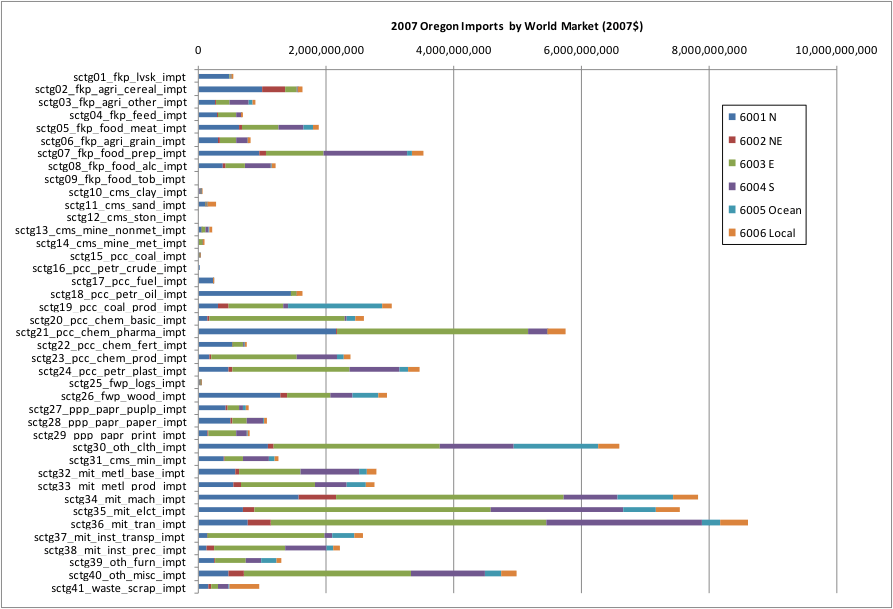
\includegraphics[width=6.0in]{aa/world-imports}
\caption{Assumed world market imports market share}\label{fig:aa-world-imports}
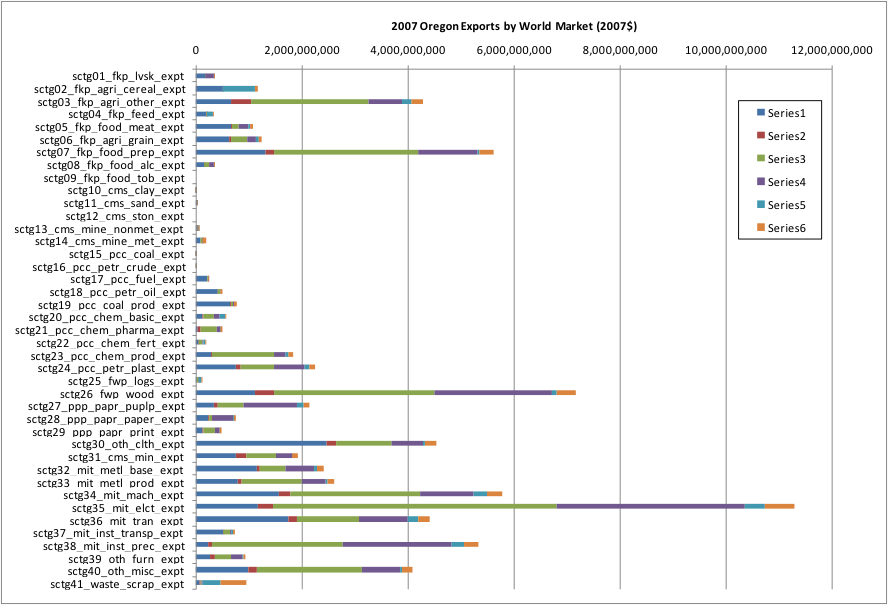
\includegraphics[width=6.0in]{aa/world-exports}
\caption{Assumed world market exports market share}\label{fig:aa-world-exports}
\end{figure}
 
\subsection{Trip Length Targets}\label{sec:aa-trip-length-targets}
Observed trip length distances were collected to compare with AA commodity flow outputs. An automated trip length calibration routine uses targets in the file histogramsI.csv and outputs comparable distributions in histograms.csv, and resulting updates to dispersion parameters in CommoditiesI.csv.

\subsubsection{Commodity Trip Distances}
For freight, the FAF data provides 2007 average distances by SCTG commodity, as shown in Figure \ref{fig:aa-faf-distances}. This includes only trips within Oregon by value for all modes (dropped ``Pipeline'' and ``Other unknown'' modes). FAF3 has two Oregon zones, with intrazonal distances assumed to be 25 miles for ``Portland Oregon'' FAF zone and 215 miles for ``Oregon Remainder'' FAF zone (based on average of non-Portland OD pairs mileage table [50]) and 153.72 miles between them. Because of this coarse geography and the fact that FAF, based on the US CFS, primarily addresses long-distance travel and average distances vary significantly between years, the data are not ideal. It is most important to calibrate the trips internal to the model area, excluding imports and exports. 

\begin{figure}    % Formerly Figure 6.9
\centering
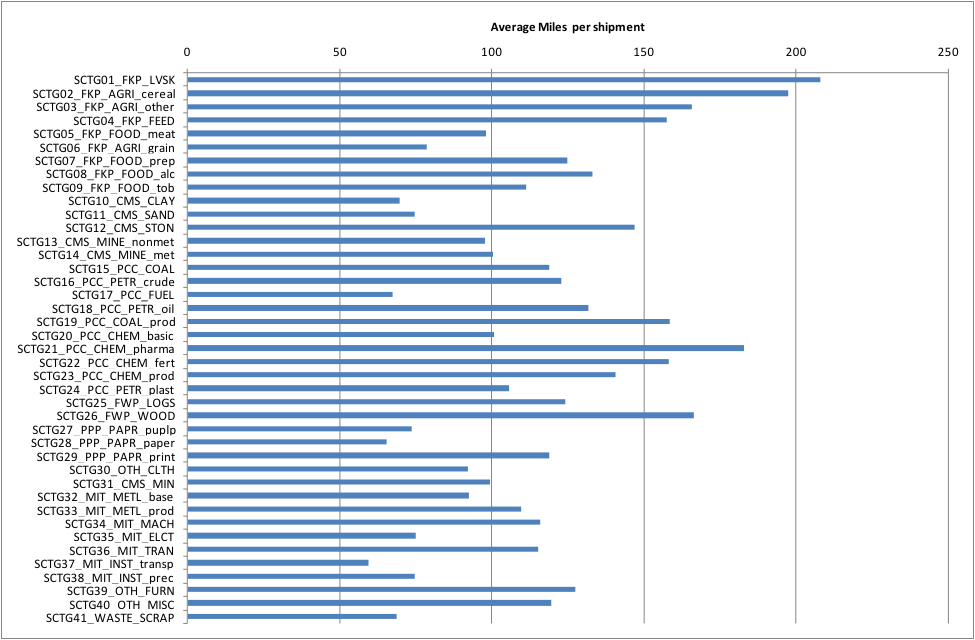
\includegraphics[width=6.0in]{aa/faf-distances}
\caption{FHWA FAF3 average commodity trip distance in Oregon}
\label{fig:aa-faf-distances}
\end{figure}

\subsubsection{Person Trip distance distribution}
The combined 1994 and 1996 Oregon Travel Behavior Surveys collected household activity data from the four Oregon MPO areas (Metro, M-WVCOG, LCOG and RVCOG) and eight additional rural Oregon counties (Clatsop, Coos, Deschutes, Josephine, Klamath, Lincoln, Malheur and Umatilla) as shown in Figure \ref{fig:aa-obts-map}. Eighty percent of the sampled trips were by auto. 

\begin{figure}[!t]    % Formerly Figure 6.10
\centering
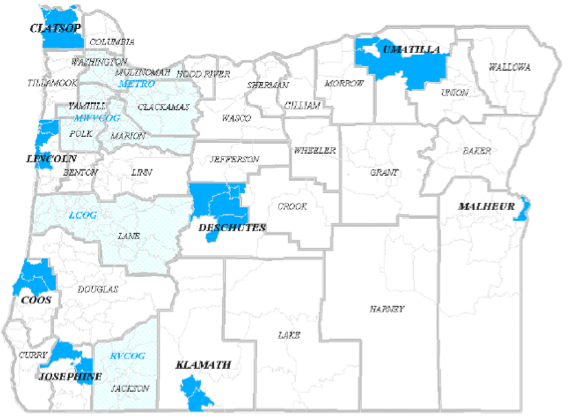
\includegraphics[width=4.0in]{aa/otbs-map}
\caption{Map of Oregon Travel Behavior Survey surveyed areas}
\label{fig:aa-obts-map}
\end{figure}

These observed trip lengths will be used to assess AA person flow outputs. Survey data on the first link of each trip tours is broken out by purpose with work trips further delineated by occupation. These will be compared to work commute and personal services trip distances, output from the AA module. Services are broken into personal and business categories, based on their primary activity, as shown in Table \ref{tab:activity-industry} (page \pageref{tab:activity-industry}). The personal distance distributions are shown in Figure \ref{fig:aa-personal-distance}. The figure indicates that most Oregon person tips are less than five miles. Work trips are the shortest in length. Portland has less of the shortest work trips (less than 2.5 miles). This concurs with a separate source, Portland DOT fact sheet that reports an average (home-based) work trip of 6.6 mile in Portland.

\begin{figure}    % Formerly Figure 6.61
\centering
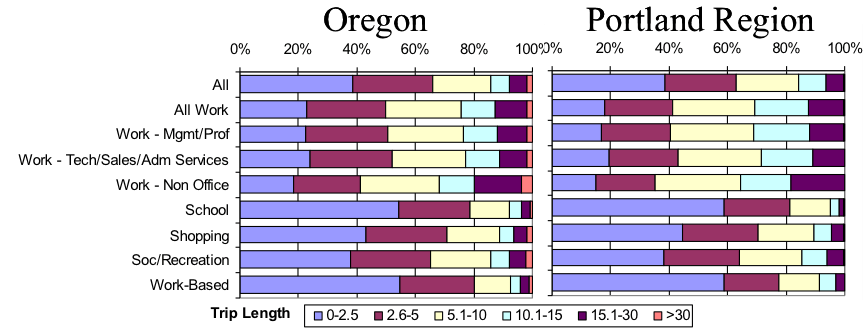
\includegraphics[width=6.0in]{aa/personal-distance}
\caption{Map of Oregon Travel Behavior Survey surveyed areas}
\label{fig:aa-personal-distance}
\end{figure}

Average business-related service trip lengths will be generated by combining the 1994/1996 Oregon household survey data with Ohio Business Establishment survey data. Business-related service trips were isolated from the Oregon data by industry and will be checked against Ohio data. 

\subsection{Floorspace Price Targets} 
Floorspace prices by building type provide general targets to assess residential and commercial floorspace prices inAA outputs by beta zone. The 2000 census provided data on residential space, while commercial rents were obtained from a sample of observed sales.  

\subsubsection{Residential Floorspace Price Targets}
2000 Census data were used to estimate residential floorspace rents. The estimates included two sets of values; a zone-specific base rent, and a set of local effect factors that adjust this base rent to reflect the local influences that act at a geographic level smaller than the zone system. The latter is useful in a land use micro-simulation model, such as the PECAS Space Development (SD) module. By separating the two elements, a more unbiased estimate can be obtained for the zonal rent, used as the AA target. 

A full discussion of the theory and mathematics behind this estimation is discussed in [53]. In general, a synthetic population of housing units was created for the entire model region. It was derived through a simulated annealing process using 2000 Census SF3 (Summary file 3) data at a block group level, which served as marginals, matched with 2000 PUMS (5 percent) disaggregate data. American Community Survey data was used to convert Census number of rooms to building sqft. A gross rent for the entire block group (SF3) was used to scale the PUMS-based rents. 

The second step isolated three local rent effects: the distance to major roads, the distance to water, and the local density. These were all calculated by census block. The first two assumed a 10 mile buffer analyses, while the density measure was defined as the number of housing units within 0.25 miles of the block. Each block was assumed to have a constant density of housing units, and the portion of each block within the buffer was used to determine this value. 

An ordinary least squares procedure with a linear model was used to estimate the local effects shown in Table \ref{tab:res-rent-regression}. The constant or base price in each zone is show graphically in Figure \ref{fig:aa-base-rents}.

\begin{figure}[!t]
\centering
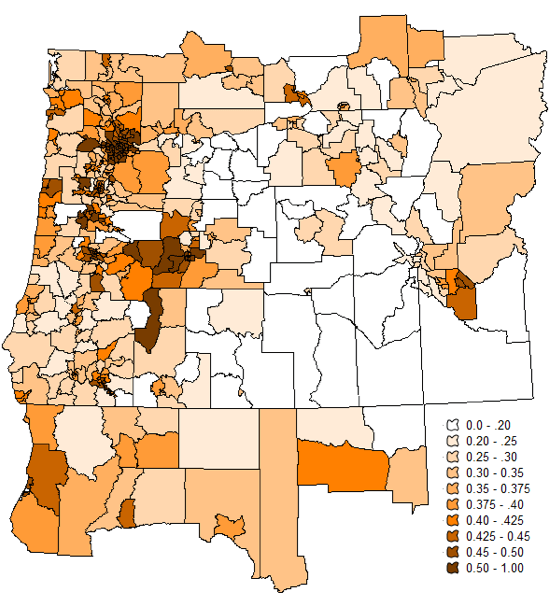
\includegraphics[scale=0.6]{aa/figure6-7alt}   % figure number mis-numbered in original text
\caption{Base rent (\$/sqft) for modeled area}\label{fig:aa-base-rents}
\end{figure}

\begin{table}
\centering
\caption{Residential rent regression}\label{tab:res-rent-regression}
\begin{tabular}{lrr}
\hline
Regression & Coefficient & Intercept \\
\hline
MH & 1.103516503 & 960996.2 \\
\gray RRMH & 0.327002266 & 1797385 \\
SFD & 1.341969751 & -1245254 \\
\gray RRSFD & 0.574700142 & 150677.6 \\
\hline
\end{tabular}
\end{table}

The higher values for mobile home and multifamily can be attributed to the larger size per unit for these dwelling types. The constant for age is negative reflecting the expected reduction of value of buildings with age. The constant for density is positive, which may reflect multiple trends. In a large city, accessibility can be thought of as the distance to the downtown, shopping centers and services. However, in smaller towns, accessibility is as much the distance to Main Street and to other towns and cities.Water has a larger parameter than proximity to major road in these estimations. All rents are in the same money units used by the census, dollars per month, calculated on a per square foot basis.

The base prices by zone are consistent with expectations; the rural areas of eastern Oregon and the halo have the lowest rent values, and the major urban areas have the highest, and especially the south-western suburbs. The high base rents for the rural areas to the west of Bend are unexpected. The two highest rent zones in the area also have a very low number of observations, which is likely playing a role in these values. A revisiting of the rent prices in these areas by a more manual intervention may be necessary.

When used as targets for AA calibration, the base price for each beta zone was modified by the average value of each local variable (density, distance to water, distance to road, from the 2000 Census) using the rent modified coefficients of Table \ref{tab:res-rent-regression}. This modified base price was extended to the various floorspace types based on regressions of 1998-PI floorspace target data relative to the average price for that type. The regression results are given in Table \ref{tab:resulting-rent-parameters}, and the resulting parameters applied to the modified base for each type is given in Table \ref{tab:residential-modifiers}, with average rents by region shown in Figure \ref{fig:average-res-rents}. For comparison with AA outputs (ExchangeResultsI.csv ``price''), the prices are in units of amortized annual prices (\$/sqft) in 2009 dollars.

\begin{table}
\centering
\caption{Resulting residential rent parameters applied to modified base rent}
\label{tab:resulting-rent-parameters}
\begin{tabular}{lrr}
\hline
Combined & Coefficient $\times$ base (\$M) & +Intercept \\
\hline
RES-AT & 0.902685344 & 0 \\
\gray RES-MF & 1.325467507 & 0 \\
RES-MH & 1.205775939 & 960996.2 \\
\gray RES-RRMH & 0.357304547 & 1797385 \\
RES-SFD & 1.341969751 & -1245254 \\
\gray RES-RRSFD & 0.574700142 & 150677.6 \\
\hline
\end{tabular}
\end{table}

\begin{figure}
\centering
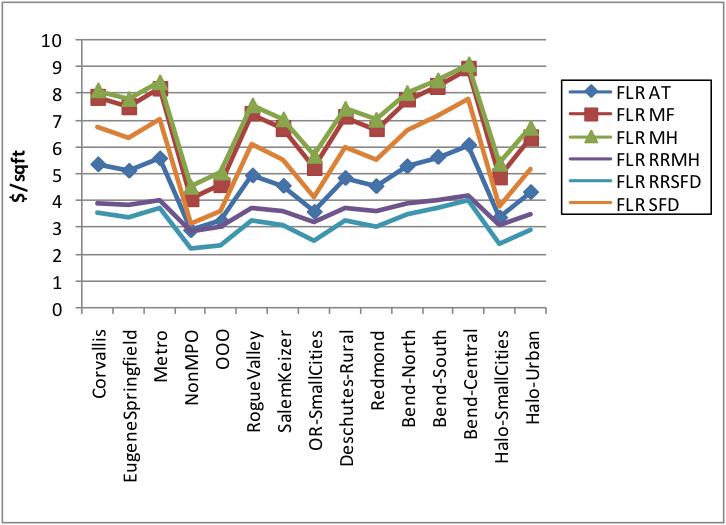
\includegraphics[scale=0.45]{aa/figure6-8alt}   % Mis-numbered in original document
\caption{Average residential rents (\$/sqft) by region}\label{fig:average-res-rents}
\end{figure}

\begin{sidewaystable}    % Table 6-23 Residential Rent Modifier Parameters
\centering
\caption{Residential rent modifier parameters}\label{tab:residential-modifiers}
\begin{tabular}{llcccc}
\hline
 & & & Estimated & T-ratio for & Corresponding \\
Parameter & Form & RefDValue & value for $a_g$ & estimated $a_g$ value & value for $\omega_g$ \\
\hline
Attached single family dummy & Constant & n/a & -0.0973 & 8.50 & 0.907 \\
\gray Multifamily dummy & Constant & n/a & 0.3255 & 54.53 & 1.384 \\
Mobile home dummy & Constant & n/a & 0.0927 & 8.67 & 1.097 \\
\gray Density & Reversed Power & 1 & 0.000103 & 10.47 & -0.000103 \\
Distance to water (feet) & Shifted exponential & 2640 & 0.0395 & 5.10 & 0.0395 \\
\gray Distance to road (feet) & Shifted exponential & 2640 & 0.0872 & 5.47 & 0.0872 \\
\hline
\end{tabular}
\end{sidewaystable}

\subsubsection{Commercial Floorspace Price Targets}
Observed non-residential prices were collected for key locations within the study area to compare with AA commodity price outputs. Floorspace prices were obtained from Real Estate Market reports for key urban areas (Bend-Deschutes [54], Portland [55], Salem-Keizer, Eugene-Springfield, Rogue Valley, Corvallis) and selected rural areas (Oregon Small Cities) within Oregon. Urban areas within the halo adopted average of Salem, Eugene, Rogue Valley and Corvallis. Non MPO in Oregon or the halo assumed 90 percent of the prices of the Oregon Small Cities data. All data was collected for the years 2009-2011 and converted to 2009 dollars.

Selected rent data, typically from the web for one or a couple areas within each region (Deschutes-Bend)was downloaded and processed. A linear regression was then performed for each of the basic space types for which data was available: office, retail, warehouse and industrial. In Deschutes County (Bend) ``warehouse'' floorspace prices were not available, so the same Office-Whse-Ind price relationship found in non-Metro MPOs was assumed. In Portland, Retail was not available, so 110 percent of the average Salem, Eugene, Rogue Valley, Corvallis Retail rates were assumed.

The variation in the observed basic type prices across the regions is shown in Figure \ref{fig:aa-basic-floorspace-prices}. These regional prices were then disaggregated to zones. In the Portland area, all zones had observed prices for the basic types which were used directly. In some cases, a few holes were filled by adopting prices from adjacent areas. In other areas, the relationship of prices across zones within the regions from 1998 PI-based floorspace price targets were used to arrive at average zone prices. To do so, average 1998 prices for all types in each MPO was generated. Then the ratio of the zonal target price to the average price in this 1998 data was calculated. This 1998 price ratio was applied as a scalar to the observed 2009 average MPO prices to arrive at zone-specific prices. 

\begin{figure}    % Formerly Figure 6.14
\centering
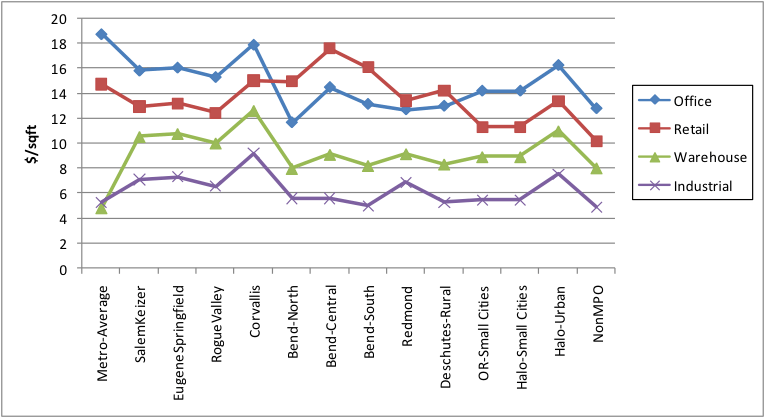
\includegraphics[width=6.0in]{aa/basic-floorspace-prices}
\caption{Basic floorspace prices by region}
\label{fig:aa-basic-floorspace-prices}
\end{figure}

Once these basic floorspace types were covered, they were extended to cover the other AA nonresidential space types. Accommodations, Government Support, K12, Hospital, and Institutional adopted ``Office'' prices. Heavy and Light industry both adopted ``Industrial'' prices. Agriculture and Logging lands assumed \$15,000 per acre. The same 1998-zonal pattern scaling noted above was also used on these non-basic floorspace types, which was often not the same pattern as the basic type (e.g., office and accommodation price scalars might differ). No zone's price was allowed to drop below a minimum price set at 50 percent of the $ExpectedPrice$ defined in AA input file CommoditiesI.csv. Figure \ref{fig:aa-retail-floorspace-prices} shows the average floorspace price for all types across the regions.

\begin{figure}    % Formerly Figure 6.15
\centering
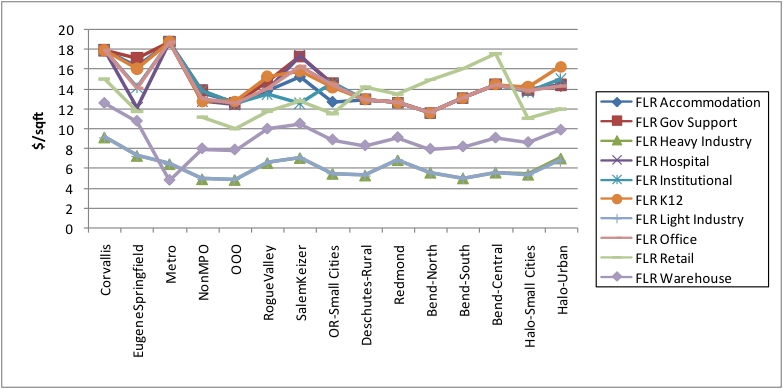
\includegraphics[width=6.0in]{aa/retail-floorspace-prices}
\caption{Retail and industry floorspace prices}
\label{fig:aa-retail-floorspace-prices}
\end{figure}

For comparison with AA outputs (ExchangeResultsI.csv ``price''), the prices are in units of amortized annual prices (\$/sqft) in 2009 dollars. 

\subsection{Commodity and Labor Flow Targets}

\subsubsection{Commodity Flow Targets}
The FHWA Freight Analysis Framework (FAF3)provides 2007 data on the flow (in dollars) of commodity movements in, out, and within the state (see \S\ref{sec:aa-trip-length-targets} for data description used in commodity trip distances). This target data, summarized in Table \ref{tab:aa-faf3-flows}, can be compared to AA flow matrices for each commodity (selling\_SCTG*.zmx). Note that these data are independent of the IMPLAN data used in NED that is used to define the overall quantity of flow in NED and AA. As such, it might be more useful to compare relative values only.

%Table 6-26 2007 FAF3 Flows, in, out, within Oregon (2007$)
\begin{table}
\centering
\caption{FAF3 flows in, out, and within Oregon, in 2007 dollars}
\label{tab:aa-faf3-flows}
\small
\begin{tabular}{lrrrr}
\hline
Commodity & OR imports & OR exports & Within OR & \% local \\
\hline
SCTG01\_FKP\_LVSK & 513,050,125 & 339,096,909 & 779,891,461 & 48 \\
\gray SCTG02\_FKP\_AGRI\_cereal & 1,545,018,337 & 1,111,557,953 & 1,488,285,000 & 36 \\
SCTG03\_FKP\_AGRI\_other & 845,320,641 & 4,065,851,489 & 2,911,841,018 & 37 \\
\gray SCTG04\_FKP\_FEED & 664,711,113 & 326,681,597 & 503,585,800 & 34 \\
SCTG05\_FKP\_FOOD\_meat & 1,788,122,165 & 1,022,702,207 & 1,181,970,878 & 30 \\
\gray SCTG06\_FKP\_AGRI\_grain & 769,284,881 & 1,188,071,419 & 1,020,120,942 & 34 \\
SCTG07\_FKP\_FOOD\_prep & 3,350,738,063 & 5,343,447,509 & 3,082,694,560 & 26 \\
\gray SCTG08\_FKP\_FOOD\_alc & 726,571,165 & 286,444,705 & 1,447,450,506 & 59 \\
SCTG09\_FKP\_FOOD\_tob & 412,899,085 & 48,404,201 & 379,892,196 & 45 \\
\gray SCTG10\_CMS\_CLAY & 37,812,001 & 4,620,401 & 350,062,484 & 89 \\
SCTG11\_CMS\_SAND & 59,452,701 & 1,843,201 & 109,890,700 & 64 \\
\gray SCTG12\_CMS\_STON & 74,850,001 & 16,003,401 & 415,626,908 & 82 \\
SCTG13\_CMS\_MINE\_nonmet & 167,393,601 & 47,053,001 & 90,622,700 & 30 \\
\gray SCTG14\_CMS\_MINE\_met & 58,180,301 & 132,194,389 & 2,076,300 & 1 \\
SCTG15\_PCC\_COAL & 13,515,601 & 983,501 & 427,400 & 3 \\
\gray SCTG16\_PCC\_PETR\_crude & 3,001 & 1,219,101 & 38,400 & 3 \\
SCTG17\_PCC\_FUEL & 226,259,305 & 226,376,893 & 4,383,043,934 & 91 \\
\gray SCTG18\_PCC\_PETR\_oil & 1,539,768,017 & 472,512,945 & 2,224,503,352 & 53 \\
SCTG19\_PCC\_COAL\_prod & 2,871,767,635 & 729,500,901 & 1,316,688,412 & 27 \\
\gray SCTG20\_PCC\_CHEM\_basic & 2,458,215,841 & 551,407,317 & 324,965,204 & 10 \\
SCTG21\_PCC\_CHEM\_pharma & 5,466,607,993 & 472,270,065 & 1,875,274,588 & 24 \\
\gray SCTG22\_PCC\_CHEM\_fert & 720,969,461 & 177,694,701 & 308,502,492 & 26 \\
SCTG23\_PCC\_CHEM\_prod & 2,267,072,461 & 1,753,345,167 & 1,108,440,494 & 22 \\
\gray SCTG24\_PCC\_PETR\_plast & 3,286,987,819 & 2,143,697,529 & 1,453,720,704 & 21 \\
SCTG25\_FWP\_LOGS & 36,885,701 & 100,623,601 & 31,785,300 & 19 \\
\gray SCTG26\_FWP\_WOOD & 2,808,749,743 & 6,817,147,673 & 4,381,969,470 & 31 \\
SCTG27\_PPP\_PAPR\_puplp & 737,031,217 & 2,037,525,443 & 533,900,984 & 16 \\
\gray SCTG28\_PPP\_PAPR\_paper & 1,017,084,169 & 715,366,965 & 1,420,600,320 & 45 \\
SCTG29\_PPP\_PAPR\_print & 761,453,121 & 456,695,801 & 1,059,349,408 & 47 \\
\gray SCTG30\_OTH\_CLTH & 6,261,516,743 & 4,320,955,781 & 2,416,852,162 & 19 \\
SCTG31\_CMS\_MIN & 1,190,854,565 & 1,824,193,491 & 3,267,382,790 & 52 \\
\gray SCTG32\_MIT\_METL\_base & 2,641,014,089 & 2,287,099,785 & 1,937,415,332 & 28 \\
SCTG33\_MIT\_METL\_prod & 2,624,619,071 & 2,487,989,665 & 3,014,642,272 & 37 \\
\gray SCTG34\_MIT\_MACH & 7,437,560,381 & 5,501,173,891 & 10,637,128,772 & 45 \\
SCTG35\_MIT\_ELCT & 7,163,601,851 & 10,729,985,303 & 5,043,549,094 & 22 \\
\gray SCTG36\_MIT\_TRAN & 8,184,706,297 & 4,192,043,773 & 3,915,328,320 & 24 \\
SCTG37\_MIT\_INST\_transp & 2,441,527,765 & 710,298,437 & 208,094,604 & 6 \\
\gray SCTG38\_MIT\_INST\_prec & 2,107,658,451 & 5,065,495,549 & 445,596,792 & 6 \\
SCTG39\_OTH\_FURN & 1,225,939,257 & 895,793,341 & 791,336,400 & 27 \\
\gray SCTG40\_OTH\_MISC & 4,738,775,085 & 3,890,551,997 & 1,854,959,488 & 18 \\
SCTG41\_WASTE\_SCRAP & 477,999,877 & 475,325,865 & 1,385,731,402 & 59 \\
\gray SCTG43 Mixed miscellaneous$^a$ & 4,500,276,391 & 6,907,573,625 & 9,058,693,880 & 44 \\
\hline
Total & 86,221,825,088 & 79,878,820,488 & 78,163,933,223 & 32 \\
\hline
\multicolumn{5}{l}{\footnotesize a. Included in FAF3 data, but not used by AA.}
\end{tabular}
\end{table}


\subsubsection{Labor Flows Targets}
Labor flow targets from 2000 US Census PUMS data, in units of wages by occupation between PUMA (home-to-place of work) were process as a target for AA labor flows. PUMS data was chosen over county-level US Census CTPP data since CTPP is classified by wages per household not occupation used in AA. This target can be compare to SWIM2 AA output flow matrices (\$labor\_occupations\$.zmx), collapsing beta zones to match PUMAs and occupations, and adjusting for 2009 dollars. Further discussion of this PUMS dataset can be found in \S\ref{sec:aa-zonal-activity-targets} with the employment by industry, including Figure \ref{fig:aa-synthesis-geographies} showing maps of PUMA boundaries within the study area.

In the PUMS data, place of residence is ``Puma'' and place of work is ``POWPuma''. Blank POWPumas were dropped, indicating that the person is Civilian employed with a job but not at work, currently unemployed, or not in labor force. In aggregating wage data, it was weighted by the number of employed persons. 

\section{Initial Calibration}\label{sec:aa-initial-calibration}
A formal four tier calibration strategy was employed to assess the fit of the AA module in the second stage (S2) of the calibration process, with additional informal checks by ODOT. The set of calibration procedures that was used is described below, along with further improvements that could be made to the calibration.
\begin{enumerate}
\item Convergence and Zonal Activity Totals
\begin{enumerate}
\item Zonal constants were fine-tuned to match zonal activity targets (household counts and worker activity dollars).
\item Modelwide imports and exports were calibrated and constants in the world market adjusted to match these targets.
\item AA was assembled and run to convergence. After the results of this run were reviewed, the activity dispersion parameters (in ActivitiesI.csv) were updated. The industry parameters were borrowed from Baltimore, where they had been calibrated to elasticity on space use.  The household parameters were borrowed from California, where they were based on combinations of nesting rules and elasticity tests. Labor occupation choice was investigated further to determine whether there was appropriate spatial labor specialization around job locations, using Census PUMA level targets for occupations. The model was rerun to convergence constrained to zonal activity totals. The prices were high for some non-residential space types, a problem that was revisited in floorspace price calibration.
\end{enumerate}
\item Trip lengths were checked against previous 1998 targets for services and labor, and updated FAF3 goods trip length targets. A semi-automated routine was developed to perform the calibration, and the AA input files were updated. Modifications that had been previously made to the transport coefficients to match trip length targets were revisited, to understand overall flow length distributions and their economic implications. The census question details regarding trips to work were investigated; very long distances between home and workplace are unlikely to be reported in Census, which focuses on the usual journey to work.  Further investigation could occur using other labor market surveys. At this stage the labor flow distances in PECAS seem appropriate but are somewhat longer than observed average trip lengths, and it is suggested that this be addressed further in the transportation models so that trip-to-work distributions can be shorter than labor-flow distributions.
\item Prices: reasonable values for floorspace and labor prices:
\begin{enumerate}
\item Technology option cluster weights were calibrated so that household chose their technology cluster points in the correct amounts (use of dwelling type, dwelling size, make of labor occupations) and so that industries chose the correct amount of space overall (use of labor and floorspace).
\item Floorspace inventory were adjusted so the resulting model reproduced floorspace price targets, while maintaining the correct amount of activity within the zone (zonal activity constants calibration). An automated script was used to adjust the initial synthesized floorspace quantities by Alpha Zone. This script automates the process of finding a best match to both inventory and price data while retaining the zonal activity of Step 1. This calibration script was was instrumental in discovering a mismatch between housing data and census population data. The resulting model's match to rent targets and total inventory targets was mapped and plotted and discussed by the team, and the matches were deemed appropriate.  Vacancy rates may also be reviewed in full model calibration.
\end{enumerate}
\item Technology option choice dispersion parameters were adjusted for households based on occupation choice targets. In general, they were not changed much from their previous values from December of 2012.
\item Commodity flows
\begin{enumerate}
\item Labor flows can be checked against POWPUMA-PUMA flow targets by occupation.
\item Goods commodity flows into/out of/through the state can be compared against FAF3 targets in total and/or by aggregated commodities where possible.
\end{enumerate}
\item Check household trends over time by comparing SPG household size (SynPopP.csv + SynPopH.csv) trends over time, to Portland Metro forecast/other sources.
\end{enumerate}

The calibration targets used to assess the model fit during calibration were previously listed in Table \ref{tab:aa-calibration-targets}. The following AA Validations of special interest to ODOT. The first two are part of the calibration noted above, while the last one can be included if ODOT leads the comparison effort:
\begin{itemize}
\item High Prices of selected space types (Office, Warehouse, Light Industry, Retail, Grade School, Government Support) are current PI-ALD issue in SWIM2. Some spaces will likely not be market sensitive and/or limited quantities result in counterintuitive prices (schools, government, hospitals), but prices for common space types should not be unreasonably high. (See AA calibration step 5)
\item Long Distance Commuting is important for GHG reduction strategies. Not a focus in prior PI calibration (when comparing CTPP county-county labor flows, $R^2$ was high since matched larger short commutes, but did not match well against smaller long distance flows and HH survey not capture either). New OHAS survey data that includes long commutes will help, possibly Census OnTheMap data as well. (See AA calibration step 3). AA does not represent commuting distance, only a financial relationship between an employer and an employee. PT uses the financial relationship to forecast commuting trips. Properly accounting for long distance commute trips may require an adjustment of PT which is beyond the scope of the current project.  
\item Matching HHSize changes: PI/AA is calibrated to households, not population, so household size trends are not controlled. In Oct 2010 model runs, SWIM2 predicted reasonable HH forecasts compared to Portland Metro model runs, but overall population was larger due to SWIM2 forecast of larger HH sizes (consistent with Census trends for increased workers per HH). SWIM2 also predicted Eastern Oregon average household size would grow over time, while the rest of Oregon shrunk.  Additionally, a ``stepped'' growth in household size changes was observed (might be due to recent ALD changes). ODOT is encouraged to update these comparisons with the updated SWIM2 spatial models during calibration, where issues can be discussed appropriate action can be taken, if required.
\end{itemize}

Calibration Step 3 is discussed in more detail below:

\subsubsection{Iterative floorspace calibration}

The use of synthesized floorspace inventory directly proved to be excessively large (high vacancy rates) and resulted in homogenous prices across all zones. As a result, an involved process is used to iteratively trim the floorspace quantities while constraining the process to meet the following targets:
\begin{itemize}
\item Modelwide vacancy rates by floorspace type from 2000 Census (residential) and mid-1990s real estate sales reports (nonresidential).
\item Modelwide activity use of each residential floorspace type from 2000 Census PUMS(sqft/HH).
\item Alpha zone-level floorspace prices by floorspace type (\$/building sqft) from mid-1990s real estate sales reports (selected urban areas) and early 1990s Tax Assessor Data used in SWIM1 model development (outside urban areas, converted from \$/land sqft).
\end{itemize}

The process involves iteratively running the AA module as follows. The resulting floorspace more accurately represented both floorspace price variations and vacancy rates: 
\begin{itemize}
\item Reduce floorspace inventory to match target modelwide vacancy rates by floorspace type (alpha zone).
\item Iteratively calibrate AA modelwide activity use of floorspace type (offset parameters) while constraining to alpha zone activity targets. To save runtime, this was first done at a county zone level and then the county offsets were transferred to the more disaggregate beta zone level for fine tuning.
\item As needed, adjust the floorspace inventory to match target modelwide floorspace price targets. This tended to reduced price outliers caused by the above steps, but worked against reducing vacancy rates.
\item Repeat additional adjustments to floorspace inventory to match target modelwide vacancy rates (and to a lesser extent zonal floorspace prices), as needed, repeating this multi-step process until vacancy rates were within the target range and prices were reasonable.
\end{itemize}

This process was applied to all nonresidential floorspace types and single-family (SFD) residential floorspace type. Residential calibration was complicated by the fact that all household types are allowed to use multiple floorspace types. However since residential space in the model is dominated by SFD type, the above adjustments were made to SFD only. The inventory of other residential floorspace types was derived from the resulting SFD space based on 2000 Census mix of dwelling units in each alpha zone.

\section{Further Calibration}
Additional rounds of calibration were performed after data discrepancies were found and corrected. First, after initial calibration revealed a mismatch between housing data and population data in Clark County, Washington, the following calibration steps were performed on the corrected model:
\begin{enumerate}
\item Household cluster weights were calibrated so that household activities were allocated to clusters in the correct proportions. This was done using an autonomous script that iteratively ran AA and adjusted the weights to bring the proportions closer to the targets. After calibration, all cluster amounts matched their targets.
\item Floorspace inventory was adjusted to better match the observed space prices without deviating too much from the existing floorspace quantities from previous calibration. This was achieved by assigning each quantity and price target a ``tolerance'' indicating how far the calibration script would allow the modeled value to deviate from the target. Since large interactions occurred between cluster weight calibration (step 1) and floorspace calibration, these two processes were run alternately until they both converged, as described below. For some space types (e.g. office, retail), only small adjustments were needed. For other types, where prices started far from the targets, larger adjustments were needed; for example, heavy industry space was decreased by half in some zones to control inflated prices in the model. In all space types, the overall fit to the targets improved.
\item Trip lengths for goods, which had deviated from their targets during other calibration steps, were re-calibrated against the FAF3 goods trip length targets. An autonomous script ran AA repeatedly, increasing the location choice dispersion parameter for each commodity to decrease the average trip length and vice versa. Labor and service trip lengths were not included in this step because dispersion parameter adjustments alone could not match the targets.
\end{enumerate}

The second round of recalibration was done after correcting errors in the household counts. Only floor space calibration was performed at this stage, using the same price targets as before. The space targets were adjusted to remove small out-of-place floorspace amounts (such as rural residential space in urban areas) and to better fit the distribution of observed activities. 

\subsubsection{Alternating cluster weight and floorspace calibration}
An automated script was developed to repeatedly run the cluster weight and floorspace calibration processes in an alternating fashion. The initial runs used relaxed convergence criteria so that they took less time, while later runs restored more demanding convergence criteria to ensure an accurate calibration.

This alternation was done because the cluster weights were calibrated assuming the original floorspace quantities. Changing the floorspace amounts affected the supply of residential floorspace, which altered the proportions assigned to each cluster. The effect on cluster distribution was so dramatic that AA would sometimes not converge at all. After alternating the two calibration routines, all household cluster amounts matched their targets, and the overall fit to floorspace quantity and price targets was improved.

\section{S3 Parameters}
When the full SWIM2 model is undergoing calibration, the following parameters may be adjusted to improve AA and overall model performance:
\begin{itemize}
\item Inertia parameters for activity location by activity type $\alpha_{inertia}$ and $InertiaConsta$.
\item Floorspace import function parameters (for calculating floorspace import functions based on floorspace inventory).
\item Multipliers for the influence of specific commodity buying and selling utility values on production location utility ($\phi$b,c,a and $\phi$s,c,a).
\item Affect of production utility and consumption utility on location utility ($\alpha_{prod,a}$ and 
$\alpha_{cons,a}$).
\item Utility of non-modeled production and non-modeled consumption ($U_{nmc}$ and $U_{nmp}$).
\item Utility function dispersion parameter for allocation of by-product substitutes and input substitutes made and used by each activity ($\lambda_{m,a}$ and $\lambda_{u,a}$).
\end{itemize}
